% !TEX program = xelatex
\documentclass[UTF8,11pt,twoside,openany,fontset=none]{ctexbook}
% Series palette and typography follow ../book/preamble.tex.
\defaultCJKfontfeatures{}
\IfFontExistsTF{SimSun}{
  \setCJKmainfont[BoldFont=SimHei,ItalicFont=KaiTi,BoldItalicFont=KaiTi]{SimSun}
  \setCJKsansfont[BoldFont=Microsoft YaHei Bold]{Microsoft YaHei}
  \setCJKmonofont{SimSun}
}{
  \setCJKmainfont[BoldFont=FandolSong-Bold,ItalicFont=FandolKai-Regular]{FandolSong-Regular}
  \setCJKsansfont[BoldFont=FandolHei-Bold]{FandolHei-Regular}
  \setCJKmonofont{FandolFang-Regular}
}
\usepackage[a4paper,inner=24mm,outer=21mm,top=24mm,bottom=24mm,headheight=16pt]{geometry}
\usepackage{lmodern,amsmath,amssymb,mathtools,bm,mathrsfs}
\usepackage[dvipsnames]{xcolor}
\usepackage[most]{tcolorbox}
\usepackage{tikz,pgfplots,booktabs,array,longtable,tabularx,multirow,enumitem,fancyhdr,graphicx}
\usetikzlibrary{arrows.meta,positioning,calc,decorations.pathreplacing}
\usepackage{caption,subcaption,listings,etoolbox,float}
\usepackage{multicol,titletoc}
\usepackage{hyperref,cleveref}
\pgfplotsset{compat=1.18}
\definecolor{Ink}{HTML}{19364A}
\definecolor{Teal}{HTML}{227C81}
\definecolor{Gold}{HTML}{A87830}
\definecolor{Rust}{HTML}{9B483A}
\definecolor{CoverTeal}{HTML}{20B2AA}
\definecolor{ContentsBlue}{HTML}{3675BF}
\definecolor{CoverGray}{HTML}{7A7A7A}
\definecolor{PetalGold}{HTML}{D9C32D}
\hypersetup{colorlinks=true,linkcolor=Teal,urlcolor=Teal,citecolor=Teal,bookmarksnumbered=true,pdftitle={概率论与数理统计考研与竞赛复习册},pdfauthor={雪落长安无声},pdfsubject={概率论与数理统计教材}}
\ctexset{chapter={format=\Huge\bfseries\color{Ink},beforeskip=10pt,afterskip=22pt},section={format=\Large\bfseries\color{Teal}},subsection={format=\large\bfseries\color{Ink}}}
\ctexset{chapter/tocline={\CTEXifname{\protect\numberline{\thechapter}}{}#2}}
\setcounter{tocdepth}{2}
\setcounter{secnumdepth}{2}
% book's mainmatter uses cleardoublepage even with openany; avoid an inserted verso.
\patchcmd{\mainmatter}{\cleardoublepage}{\clearpage}{}{%
  \PackageError{book_probability}{Could not disable the mainmatter blank page}{Check the definition of mainmatter.}}
\titlecontents{chapter}[1.8em]
  {\addvspace{6pt}\bfseries\color{black}}
  {\contentslabel{1.8em}}{\hspace*{-1.8em}}
  {\hfill\contentspage}
\titlecontents{section}[3.0em]
  {\color{black}}
  {\contentslabel{2.2em}}{\hspace*{-2.2em}}
  {\color{ContentsBlue}\titlerule*[.65pc]{.}\color{black}\contentspage}
\titlecontents{subsection}[4.5em]
  {\footnotesize\color{Ink!80}}
  {\contentslabel{3.1em}}{\hspace*{-3.1em}}
  {\color{ContentsBlue!75}\titlerule*[.65pc]{.}\color{Ink!80}\contentspage}
\makeatletter
\renewcommand{\tableofcontents}{%
  \clearpage\begingroup
  \ctexset{chapter={format=\centering\LARGE\bfseries\color{ContentsBlue},beforeskip=0pt,afterskip=20pt}}%
  \chapter*{目录}\markboth{目录}{目录}%
  \pdfbookmark[0]{目录}{book-contents}%
  \hypersetup{linkcolor=black,linktoc=all}%
  \setlength{\columnsep}{9mm}%
  \setlength{\parskip}{0pt}%
  \fontsize{10}{14}\selectfont
  \begin{multicols}{2}\raggedcolumns
    \@starttoc{toc}%
  \end{multicols}%
  \clearpage\endgroup
}
\makeatother
\pagestyle{fancy}\fancyhf{}
\fancyhead[LE,RO]{\small\color{Ink}\thepage}
\fancyhead[LO]{\small\nouppercase{\leftmark}}
\renewcommand{\chaptermark}[1]{\markboth{\thechapter\quad #1}{}}
\fancyhead[RE]{\small 概率论与数理统计 · 考研与竞赛}
\fancyfoot[C]{\scriptsize\color{Teal}概念体系\quad /\quad 多解训练\quad /\quad 证明方法}
\renewcommand{\headrulewidth}{0.4pt}
\fancypagestyle{plain}{\fancyhf{}\fancyfoot[C]{\small\thepage}\renewcommand{\headrulewidth}{0pt}}
\tcbset{enhanced,breakable,boxrule=0.45pt,arc=1mm,left=2mm,right=2mm,top=1.2mm,bottom=1.2mm,before skip=8pt,after skip=8pt,fonttitle=\bfseries,colback=white,colframe=Teal}
\newcounter{statement}[chapter]
\renewcommand{\thestatement}{\thechapter.\arabic{statement}}
\newenvironment{definition}[1]{\refstepcounter{statement}\begin{tcolorbox}[title={定义\thestatement\quad #1},colback=Teal!3]}{\end{tcolorbox}}
\newenvironment{theorem}[1]{\refstepcounter{statement}\begin{tcolorbox}[title={定理\thestatement\quad #1},colframe=Ink,colback=Ink!3]}{\end{tcolorbox}}
\newenvironment{lemma}[1]{\refstepcounter{statement}\begin{tcolorbox}[title={引理\thestatement\quad #1}]}{\end{tcolorbox}}
\newenvironment{corollary}[1]{\refstepcounter{statement}\begin{tcolorbox}[title={推论\thestatement\quad #1}]}{\end{tcolorbox}}
\newcounter{derivation}[chapter]
\renewcommand{\thederivation}{\thechapter.\arabic{derivation}}
\newenvironment{proof}{\refstepcounter{derivation}\begin{tcolorbox}[title={证明与推导\thederivation},colframe=Ink!40,colback=Ink!2]}{\hfill$\square$\end{tcolorbox}}
\newenvironment{method}[1]{\begin{tcolorbox}[title={方法卡\quad #1},colback=Teal!3]}{\end{tcolorbox}}
\newenvironment{warning}{\begin{tcolorbox}[title=易错警示,colframe=Rust,colback=Rust!3]}{\end{tcolorbox}}
\newenvironment{examtip}{\begin{tcolorbox}[title=考研要求与竞赛视角,colframe=Gold,colback=Gold!4]}{\end{tcolorbox}}
\newenvironment{insight}[1]{\begin{tcolorbox}[title={理解札记\quad #1},colframe=Teal,colback=Teal!3]}{\end{tcolorbox}}
\newenvironment{clevertrick}[1]{\begin{tcolorbox}[title={巧解与数形结合\quad #1},colframe=Gold,colback=Gold!4]}{\end{tcolorbox}}
\tikzset{laaxis/.style={->,Ink!65,line width=.45pt},lavec/.style={-{Stealth[length=2mm]},line width=1pt},lanote/.style={font=\small,align=center},lapt/.style={circle,fill=Teal,inner sep=1.5pt}}
\captionsetup{font=small,labelfont={bf,color=Teal},skip=6pt}
\newenvironment{extension}{\begin{tcolorbox}[title=竞赛拓展与选学提高,colframe=Gold,colback=Gold!4]}{\end{tcolorbox}}
\newcounter{example}[chapter]\renewcommand{\theexample}{\thechapter.\arabic{example}}
\newenvironment{example}[3]{\begin{tcolorbox}[step=example,label={ex:#3},title={例\theexample\quad #1\quad #2},colframe=Ink]}{\end{tcolorbox}}
% title, style, stars, label, problem, strategy, solution, method comparison, variation
\newcommand{\worked}[9]{\begin{example}{#1}{#2\;\ensuremath{#3}}{#4}
\textbf{题目}\ #5\par\smallskip
\textbf{思路}\ #6\par\smallskip
\textbf{解答}\ #7\par\smallskip
\textbf{方法点评}\ #8\par\smallskip
\textbf{易错点或变式}\ #9\end{example}}
\newcounter{exercise}[chapter]\renewcommand{\theexercise}{\thechapter.\arabic{exercise}}
\newcommand{\exercise}[3]{\par\medskip\noindent\refstepcounter{exercise}\label{q:#1}\textbf{习题\theexercise\quad #2}\quad #3\hfill\mbox{\hyperref[ans:#1]{\small 答案见\pageref*{ans:#1}页}}\par}
\newcommand{\answer}[2]{\par\medskip\noindent\phantomsection\label{ans:#1}\textbf{习题\ref{q:#1}解答}\quad #2\hfill\hyperref[q:#1]{\small 返回题目}\par}
\newcommand{\chaptermap}[4]{\begin{center}\begin{tikzpicture}[node distance=3mm, every node/.style={draw=Teal!50,fill=Teal!4,rounded corners=1mm,text width=.205\textwidth,minimum height=16mm,align=center,font=\small},>=Stealth]
\node(a){#1};\node[right=of a](b){#2};\node[right=of b](c){#3};\node[right=of c](d){#4};
\draw[->,Teal](a)--(b);\draw[->,Teal](b)--(c);\draw[->,Teal](c)--(d);
\end{tikzpicture}\end{center}}
\newenvironment{quicktable}{\small\begin{longtable}{@{}p{.17\textwidth}p{.25\textwidth}p{.24\textwidth}p{.25\textwidth}@{}}\toprule 方法&适用条件&典型信号&易错点\\\midrule\endhead}{\bottomrule\end{longtable}\normalsize}
\newcommand{\R}{\mathbb{R}}\newcommand{\C}{\mathbb{C}}\newcommand{\F}{\mathbb{F}}
\newcommand{\T}{^{\mathsf T}}\newcommand{\inv}{^{-1}}
\newcommand{\vx}{\bm{x}}\newcommand{\vy}{\bm{y}}\newcommand{\vz}{\bm{z}}
\newcommand{\vu}{\bm{u}}\newcommand{\vv}{\bm{v}}\newcommand{\vb}{\bm{b}}\newcommand{\va}{\bm{a}}
\newcommand{\vq}{\bm{q}}\newcommand{\vw}{\bm{w}}
\newcommand{\vc}{\bm{c}}
\renewcommand{\listfigurename}{图解目录}
\newcommand{\zero}{\bm{0}}
\DeclareMathOperator{\rank}{rank}\DeclareMathOperator{\tr}{tr}\DeclareMathOperator{\diag}{diag}
\DeclareMathOperator{\adj}{adj}\DeclareMathOperator{\Span}{span}\DeclareMathOperator{\im}{im}
\DeclareMathOperator{\sgn}{sgn}\DeclareMathOperator{\nul}{nullity}
\newcommand{\norm}[1]{\left\lVert#1\right\rVert}\newcommand{\abs}[1]{\left|#1\right|}
\numberwithin{equation}{chapter}
\setlength{\parindent}{2em}\setlength{\parskip}{3pt}
\setlist{nosep,topsep=4pt,leftmargin=2em}
\renewcommand{\arraystretch}{1.22}
\emergencystretch=3em
\raggedbottom
\pdfstringdefDisableCommands{\def\T{T}\def\R{R}\def\C{C}\def\bm#1{#1}}

% Probability volume: self-contained symbols and optional measure-theory boxes.
\newenvironment{measurebox}[1]{\begin{tcolorbox}[title={测度论选学\quad #1},colframe=Ink!60,colback=Ink!2]}{\end{tcolorbox}}
\newcommand{\Pp}{\mathbb P}\newcommand{\E}{\mathbb E}
\newcommand{\N}{\mathbb N}\newcommand{\Fcal}{\mathcal F}
\newcommand{\Gcal}{\mathcal G}\newcommand{\Bcal}{\mathcal B}
\newcommand{\ind}{\mathbf1}\newcommand{\dd}{\,\mathrm d}
\newcommand{\given}{\mid}\newcommand{\Normal}{\mathcal N}
\newcommand{\pto}{\xrightarrow{\Pp}}\newcommand{\dto}{\xrightarrow{d}}
\newcommand{\asto}{\xrightarrow{\mathrm{a.s.}}}\newcommand{\iid}{\overset{\mathrm{iid}}{\sim}}
\newcommand{\indep}{\mathrel{\perp\!\!\!\perp}}
\DeclareMathOperator{\Var}{Var}\DeclareMathOperator{\Cov}{Cov}
\DeclareMathOperator{\Corr}{Corr}\DeclareMathOperator{\MSE}{MSE}
\DeclareMathOperator{\Bias}{Bias}\DeclareMathOperator{\Exp}{Exp}
\DeclareMathOperator{\Pois}{Pois}\DeclareMathOperator{\Bin}{Bin}
\DeclareMathOperator{\Beta}{Beta}\DeclareMathOperator{\Ga}{Gamma}
\newcommand{\src}[1]{\par\noindent{\footnotesize\color{Ink!75}知识依据：[#1]。}\par}
\newcommand{\parthead}[1]{\par\smallskip\noindent\textbf{#1}\quad}
\allowdisplaybreaks
\pdfstringdefDisableCommands{\def\E{E}\def\Pp{P}\def\sigma{sigma}}
% Three-digit reference-page numbers need a wider contents margin.
\contentsmargin{2.2em}

\begin{document}
\frontmatter
\begin{titlepage}\thispagestyle{empty}
\pdfbookmark[0]{封面}{book-cover}
\begin{tikzpicture}[remember picture,overlay]
  \node[anchor=north,inner sep=0pt]
    at([yshift=-17mm]current page.north)
    {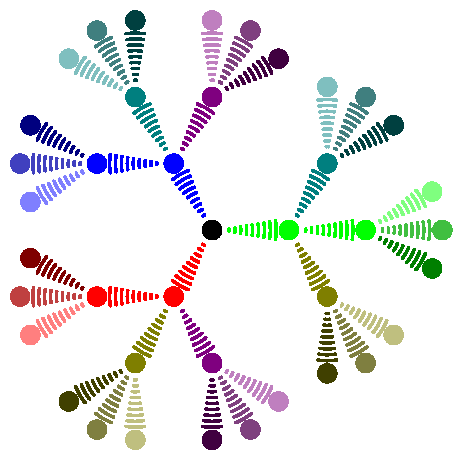
\includegraphics[width=134mm]{assets/cover-title-graphics.pdf}};
  \fill[CoverTeal]
    ([yshift=-167.9mm]current page.north west)
    rectangle ([yshift=-180.6mm]current page.north east);
  \node[anchor=north west,inner sep=0pt,align=left,text=black]
    at([xshift=12mm,yshift=-193mm]current page.north west)
    {\fontsize{27}{34}\selectfont 概率论与数理统计};
  \node[anchor=north west,inner sep=0pt,align=left,text=Ink]
    at([xshift=14mm,yshift=-209mm]current page.north west)
    {\fontsize{18}{24}\selectfont\bfseries 考研与竞赛复习册};
  \node[anchor=north west,inner sep=0pt,align=left,text=CoverGray]
    at([xshift=16mm,yshift=-229mm]current page.north west)
    {\fontsize{10.95}{18}\selectfont
      \begin{tabular}{@{}ll@{}}
        作者：&雪落长安无声\\
        邮箱：&\href{mailto:3547908579@qq.com}{\textcolor{CoverGray}{3547908579@qq.com}}\\
        时间：&2026.10.31\\
        版本：&修订版
      \end{tabular}};
  \node[anchor=center,text=black,align=center]
    at([yshift=16mm]current page.south)
    {\itshape\fontsize{10.95}{17}\selectfont 积跬步以至千里，汇微光以成星河。};
\end{tikzpicture}
\null\vfill
\end{titlepage}

\thispagestyle{empty}
\vspace*{30mm}
\begin{center}
  {\LARGE\bfseries\color{Ink}概率论与数理统计\par\vspace{6mm}考研与竞赛复习册}
  \vspace{16mm}
  {\large 数学考研与竞赛复习册系列}\par
  \vspace{10mm}
  概念体系\quad 多解训练\quad 证明方法\par
  \vspace{18mm}
  {\large 雪落长安无声}\par
  \vspace{5mm}
  \href{mailto:3547908579@qq.com}{3547908579@qq.com}\par
  \vspace{14mm}
  2026.10.31\quad 修订版
\end{center}
\vfill
\begin{center}\color{CoverGray}\small
随机模型\quad 抽样推断\quad 积分视角
\end{center}

\chapter{前言}
概率论从给定模型推导随机结果，数理统计从有限样本反推模型中的未知参数。
复习的关键是识别“随机什么、已知什么、在哪个条件下计算”。
本册把事件、分布、数字特征、极限与统计推断串成一条主线，计算旁保留条件，结论旁给出证明或可追踪的证明思路。

第1—8章覆盖考研常见核心知识；“考研核心”是学习层级标记，不声称替代某一年度、某一科目的官方考试大纲。
第9章安排方差分析与一元回归初步；第10章独立介绍测度论语言，可在完成主线后阅读。
竞赛风格题强调计数、对称、指示变量、条件分解、构造反例和多方法互证。

本册以标准概率模型、统计推断原理和可复现的数学推导组织知识。正文引用用于定位知识主题；未标为原题的训练均为本册编写的风格题。补充理论保留适用条件，重要内容配有理解札记、易错辨析和数形结合图示。

全书150个例题分别给出题目、思路、解答、点评和易错提醒；80道章末习题与答案双向链接。
多方法题的目的在于训练选择：补事件减少分类，条件化降低维数，变换揭示支撑，正交投影解释自由度。
读者可先独立解题，再对照方法点评，最后完成不同参数或不同假设下的变式。

所有图形由TikZ或pgfplots绘制，数学对象与正文同步。数字近似保留明确的近似号，精确有限样本结论与渐近结论分开标识。

\chapter{致谢}\label{front:acknowledgements}
\begingroup\small\setlength{\parskip}{2pt}
\begin{center}
  {\color{Teal}\rule{.22\textwidth}{.6pt}}\par
  \vspace{3mm}
  {\itshape 每一份清晰的理解，都建立在前人的思考与分享之上。}
\end{center}
\vspace{3mm}

本书从概念、证明、计算与解题方法四个方面整理概率论与数理统计。
在此感谢教材与讲义作者留下的系统阐述，也感谢数学学习者对严谨表达、直观解释和多种解法的持续追求。
这些积累使知识能够被反复理解、检验与传递。

\section*{参考资料与感谢}
\begin{enumerate}[label=\arabic*.,leftmargin=1.8em,itemsep=4pt]
\item \textbf{茆诗松、程依明、濮晓龙、倪菁《概率论与数理统计教程》}。
感谢其对概率模型、分布、数字特征与统计推断的系统组织，为本书概念主线提供参照。
\item \textbf{李东风《概率统计讲义》}。
感谢其对常见模型、抽样分布、参数估计、假设检验及回归方法的清晰讲解。
\item \textbf{Hao Wu（吴昊）《Introduction to Probability Theory》课程讲义}。
感谢其从可测性、积分、收敛与条件期望出发阐明概率论的理论结构。
\item \textbf{Athanasios Papoulis、S.~Unnikrishna Pillai《概率、随机变量与随机过程》}。
感谢其将概率模型、随机变量变换与应用背景相结合的叙述方式。
\end{enumerate}

感谢\LaTeX、CTeX、TikZ/PGF及相关开源社区对数学表达与书籍排版的支持。
封面配图采用Till Tantau的\href{https://texample.net/title-graphics/}{\textit{Title graphics}}数学分支图，感谢作者与TeXample社区的开放分享。
也感谢每一位认真阅读、独立演算并愿意反馈疑问的读者；对定义、条件、证明和解答的讨论，都是继续修订本书的动力。

\section*{交流与勘误}
欢迎就题目解法、公式推导与排版提出建议。反馈时可注明章节、页码或题号，便于定位与复查。
\begin{tcolorbox}[colframe=Teal!65,colback=Teal!3,boxrule=.45pt,title={联系方式}]
\textbf{作者}\quad 雪落长安无声\par\smallskip
\textbf{知乎}\quad
\href{https://www.zhihu.com/people/black-despair}{https://www.zhihu.com/people/black-despair}\par\smallskip
\textbf{QQ邮箱}\quad
\href{mailto:3547908579@qq.com}{3547908579@qq.com}
\end{tcolorbox}
\vfill
\begin{flushright}\itshape 雪落长安无声\par 2026年10月31日\end{flushright}
\endgroup

\chapter{使用说明与复习路线}
\section*{三遍阅读}
第一遍用第1—6章建立模型与分布图景，遇题先写样本空间或支撑集。第二遍完成第7—8章，把“估计量—分布—区间—拒绝域”连接起来。第三遍回到竞赛题和第9—10章，用不同方法重建结果。
\begin{center}\small
\begin{tabularx}{\textwidth}{@{}lXX@{}}\toprule
阶段&训练重点&自检标准\\\midrule
第1—2周&事件、条件概率、一元分布&能独立写事件并检查分布函数端点\\
第3—4周&多维分布、数字特征、极限&能画积分区域并说明独立性用途\\
第5—6周&抽样、估计、检验&能选枢轴量并解释自由度与尾部\\
第7—8周&回归、综合题、选学&能比较两法并检查假设改变的后果\\\bottomrule
\end{tabularx}\end{center}
\section*{盒子与题目层级}
定义和方法卡用青色；定理与例题用墨蓝；竞赛拓展和考研提示用金色；易错警示用赭色；测度论选学用浅墨色。星级从一星到三星表示本册内部相对难度。
每个知识节有3例与至少1张方法卡；章末8题依次包含基础、考研、竞赛、测度论选学各2题。点击题目后的答案页码可跳转，答案末可返回题目。
\section*{解题八问}
\begin{enumerate}
\item 样本点、随机变量或统计量分别是什么？
\item 参数空间和变量支撑是否依赖未知参数？
\item 独立、同分布、正态、有限矩分别用在哪里？
\item 是精确概率、上界，还是渐近近似？
\item 能否改求补事件、改用指示变量或先条件化？
\item 变换是否多对一，雅可比是否取绝对值？
\item 置信水平、显著性水平和分位数方向是否统一？
\item 结果能否通过总概率为1、量纲、极限或特例检查？
\end{enumerate}
\section*{统一约定}
所有分位数取左广义逆$q_u=\inf\{x:F(x)\ge u\}$；Gamma、指数均用率参数$\lambda$，若使用尺度参数$\eta$，两者关系为$\lambda=\frac{1}{\eta}$；iid表示独立同分布。测度论内容可在完成主线后阅读。

\chapter*{考研三卷种阅读路线}
\addcontentsline{toc}{chapter}{考研三卷种阅读路线}
本书覆盖面宽于统考所需内容。数学二不设置概率论与数理统计部分；数学一、三需要按各自范围阅读，不能将本书第1—10章都视为共同必修。大纲中的“考试范围”也不等于其中每个小节每年都出题。

\begin{center}
\begin{tabularx}{\textwidth}{@{}p{.38\textwidth}XX@{}}
\toprule 本书内容&数学一&数学三\\\midrule
第1—5章基础部分&按大纲读&按大纲读\\
第6章抽样及三大分布&按大纲读&按大纲读，注意典型构造\\
第6章经验分布函数&按本卷要求选读&大纲明确列入\\
第7.1节矩估计与MLE&按大纲读&按大纲读\\
第7.2节估计量评价&无偏、有效、一致等按要求读&不将全节列为共同必修\\
第7.5节区间估计&正态总体相应部分&不作本卷主线\\
第8章假设检验&检验概念与正态总体相应部分&不作本卷主线\\
第9章回归与ANOVA、第10章&提高选读&提高选读\\
\bottomrule
\end{tabularx}
\end{center}

充分完备、UMVU、信息界、Bayes、Delta 方法、测度论等按提高材料使用；不能因为它们位于基础章里，就与整个基础章一起列为统考核心。数学一的正态区间与检验也不是第7—8章所有推广题的统称。

\section*{三个已有题型的复习顺序}
\begin{enumerate}
\item \textbf{二维变换先画区域：}见第\ref{sec:33}—\ref{sec:34}节。先画联合密度支撑，明确变换不等式与零概率分母，按参数位置分段确定积分限；算出分布函数后再检查两端极限、单调性与总概率。
\item \textbf{抽样分布先列独立性：}见第\ref{sec:62}—\ref{sec:63}节。识别标准正态、独立卡方及相应自由度后再拼成 $t$ 或 $F$ 统计量。只看外形、没有独立性条件，不足以判断分布。
\item \textbf{MLE 先保留支持：}见第\ref{sec:71}节例\ref{ex:7-3}。均匀分布端点例题已经给出可行参数与样本最大值的关系，应与矩估计、正态及指数例题一起练习。无内点驻点不等于无边界最大值；点态密度版本和最大值是否取到也要核对。
\end{enumerate}

边界MLE的分类与非唯一情形见第\ref{r2:mle}节；边缘正态不推出联合正态的反例见例\ref{ex:3-15}。附录\ref{app:exam_core}提供基础题型入口，全文索引仍保留提高内容，便于后续课程使用。
范围依据为教育部教育考试院《2027年全国硕士研究生招生考试数学考试大纲》原书第20—25、45—49页。\href{https://xuanshu.hep.com.cn/front/book/findBookDetails?bookId=6aa1910be119ac97297a608f}{官方版本入口}。

\chapter{符号表}
\begin{longtable}{@{}p{.27\textwidth}p{.65\textwidth}@{}}\toprule
符号&含义与约定\\\midrule\endhead
$\Omega,\Fcal,\Pp$&样本空间、事件$\sigma$代数、概率测度\\
$A^c,\ind_A$&事件的补集、事件指示变量\\
$F_X,f_X,p_X$&分布函数、密度、离散概率质量函数\\
$F_{X,Y},f_{X,Y}$&联合分布函数、联合密度\\
$\E X,\Var(X)$&期望、方差\\
$\Cov(X,Y),\rho_{XY}$&协方差、相关系数\\
$\bar X,S^2$&样本均值与分母$n-1$的无偏样本方差\\
$X_{(k)},T,\hat\theta$&第$k$个次序统计量、统计量、参数估计量\\
$L,\ell,U,I_n$&似然、对数似然、得分、全样本Fisher信息\\
$\Phi,\varphi,z_u$&标准正态分布函数、密度及下侧$u$分位数\\
$t_{\nu,u},\chi^2_{\nu,u},F_{a,b;u}$&$t$、卡方、$F$分布下侧分位数\\
$\Normal(\mu,\sigma^2)$&均值$\mu$、方差$\sigma^2$的正态分布\\
$\Ga(a,\lambda),\Exp(\lambda)$&形状$a$、率$\lambda$的Gamma；率$\lambda$的指数分布\\
$H_0,H_1,\alpha,\beta(\theta),\pi(\theta),\psi$&原假设、备择、第一类错误水平、第二类错误概率、功效、检验函数\\
$\asto,\pto,\dto,\xrightarrow{L^p}$&几乎必然、依概率、依分布、$p$次平均收敛\\
$\Bcal(\R),\Pp_X$&实数Borel集族、$X$的分布（推前概率）\\
$\E(X\given\Gcal)$&给定子$\sigma$代数的条件期望，按几乎处处相等识别\\
$a^\mathsf T,\|a\|$&转置、欧氏范数\\\bottomrule
\end{longtable}

\tableofcontents
\listoffigures
\mainmatter
\chapter{随机事件与概率}\label{ch:01}
\chaptermap{样本空间\\事件运算}{等可能与几何\\公理化概率}{条件与分层\\全概率Bayes}{独立试验\\计数与递推}
\begin{examtip}
\textbf{考研核心：}事件表达、加法公式、条件概率、全概率、Bayes与独立性。
常考信号是“至少一次”“已知发生”“来自哪一类”。\textbf{竞赛视角：}容斥、对称、状态递推。
\textbf{测度关联：}事件必须属于可测集族，连续模型中概率为零不等于不可能。
\end{examtip}

\section{事件运算与概率公理}\label{sec:11}
\src{茆诗松, §1.1—1.3；李东风, §1.1、§1.3}
\subsection{概念与结论}
\begin{definition}{事件与概率空间}
样本空间$\Omega$是非空的可能结果集合。事件域$\Fcal$包含$\Omega$，对补集与可数并封闭，称为$\sigma$代数；事件是$\Fcal$中的集合。
$A\cup B$表示至少一个发生，$A\cap B$表示同时发生，$A\setminus B$表示$A$发生而$B$不发生。
概率是映射$\Pp:\Fcal\to[0,1]$，满足$\Pp(\Omega)=1$，且对两两不交的$A_n\in\Fcal$有
$\Pp(\bigcup_{n\ge1}A_n)=\sum_{n\ge1}\Pp(A_n)$。三者组成概率空间$(\Omega,\Fcal,\Pp)$。
\end{definition}
\begin{theorem}{加法、连续性与并集界}
$\Pp(A^c)=1-\Pp(A)$，$\Pp(A\cup B)=\Pp(A)+\Pp(B)-\Pp(A\cap B)$。
若$A_n\uparrow A$或$A_n\downarrow A$，则$\Pp(A_n)\to\Pp(A)$。
一般有$\Pp(\bigcup_n A_n)\le\sum_n\Pp(A_n)$。
\end{theorem}
\begin{proof}
把$A\cup B$拆成$A\setminus B$、$A\cap B$、$B\setminus A$即得加法公式。
对递增事件写$A=A_1\sqcup\bigsqcup_{n\ge2}(A_n\setminus A_{n-1})$，可数可加后取部分和得连续性；递减情形取补集。
任意并集先按“首次出现的下标”拆成不交事件，再逐项放大为$A_n$，即得并集界。
\end{proof}
\begin{method}{把语言翻译成互斥事件}
适用：多个事件的“仅”“至少”“恰好”。先写集合式，再用Venn区域分解，最后计算概率。
“仅$A$发生”为$A\cap B^c\cap C^c$；“恰好一个”是三个此类区域之并。
易错点：互斥是集合关系，独立是概率关系。
\end{method}
\subsection{分层例题}
\worked{恰好一个事件}{基础例题}{\star}{1-1}
{设$\Pp(A)=0.6,\Pp(B)=0.5,\Pp(A\cap B)=0.2$，求恰好一个发生的概率。}
{找对称差的两个不交区域。}
{方法一：$\Pp(A\setminus B)+\Pp(B\setminus A)=(0.6-0.2)+(0.5-0.2)=0.7$。
方法二：先算至少一个的概率$0.6+0.5-0.2=0.9$，再减同时发生的$0.2$，仍得$0.7$。}
{分区域法便于检查；先并后减适合已有并集概率时使用。}
{直接把$0.6+0.5$当答案会重复计入交集两次。}
\worked{三事件容斥}{考研风格}{\star\star}{1-2}
{三事件各有概率$\frac{1}{2}$，两两交概率均为$\frac{1}{4}$，三者交概率$\frac{1}{8}$，求至少一个发生的概率。}
{逐级纠正重复计数。}
{$\Pp(A\cup B\cup C)=\frac{3}{2}-\frac{3}{4}+\frac{1}{8}=\frac{7}{8}$。交中三者同时发生的区域在第一轮计3次、第二轮减3次，最后必须补1次。
本题数据也满足相互独立，补事件概率为$\frac{1}{8}$可作检验。}
{容斥只依赖各阶交概率，不预先要求独立。}
{只知道两两独立时，不能自动确定三重交概率。}
\worked{无放回排列的固定点}{竞赛风格}{\star\star\star}{1-3}
{随机排列$1,2,3,4$，求至少一数留在原位的概率。}
{令$A_i$为第$i$个数留在原位，对固定点使用容斥。}
{固定指定$k$个位置有$(4-k)!$种排列，故所求为
\[\dfrac{\binom41 3!-\binom42 2!+\binom43 1!-\binom44 0!}{4!}=\dfrac{15}{24}=\dfrac58.\]
其补集错排数为$9$，总数$24$。每次容斥按指定位置集合计数，因此多固定点排列的重复次数得到正确消除。}
{把多个“至少”转成容斥，复杂事件变成容易计算的交事件。}
{推广至$n$时，无固定点概率为$\sum_{k=0}^n\frac{(-1)^k}{k!}$。}

\section{古典概型与几何概型}\label{sec:12}
\src{茆诗松, §1.2；李东风, §1.2}
\begin{definition}{等可能与均匀模型}
有限等可能空间中$\Pp(A)=\frac{|A|}{|\Omega|}$。在有限正体积区域$D\subset\R^d$上均匀取点时，$\Pp(A)=\frac{\operatorname{vol}(A\cap D)}{\operatorname{vol}(D)}$。
均匀指相对于指定坐标下的体积；更换随机生成机制可能改变概率。
\end{definition}
\begin{method}{先统一计数口径}
适用：抽球、排列、抽签与几何随机点。先定有序或无序、放回或不放回；分子分母保持同一口径。
几何题先画可行域，再画事件域；均匀性未经说明时不能直接用面积比。
\end{method}
\worked{两次抽到红球}{基础例题}{\star}{1-4}
{盒中3红2白，不放回抽2球，求两球都红的概率。}
{用无序组合与逐步条件概率互证。}
{方法一：$\frac{\binom32}{\binom52}=\frac{3}{10}$。
方法二：按抽取顺序，$\Pp(R_1R_2)=\frac35\frac24=\frac{3}{10}$。
前者把一个无序球对作为样本点，后者把有序球对作为样本点，总数分别为10和20。}
{组合式短；乘法式便于处理逐次条件变化。}
{已知第一球为红时，第二球为红的条件概率为$\frac{2}{4}$；第二球为红的无条件概率仍为$\frac{3}{5}$。}
\worked{相遇问题}{考研风格}{\star\star}{1-5}
{两人独立在一小时内均匀到达，各等待15分钟，求相遇概率。}
{以小时为单位，研究单位正方形内$|x-y|\le\frac{1}{4}$。}
{不相遇区域是两块直角边长$\frac{3}{4}$的直角三角形，故概率
$1-2\cdot\frac12(\frac{3}{4})^2=\frac{7}{16}$。
另一法按第一人到达时间$x$条件化。允许的第二人到达时间区间为$[x-\frac{1}{4},x+\frac{1}{4}]\cap[0,1]$，其长度分段积分为
\[\int_0^{\frac{1}{4}}(x+\dfrac{1}{4})\dd x+\int_{\frac{1}{4}}^{\frac{3}{4}}\dfrac12\dd x+
\int_{\frac{3}{4}}^1(\dfrac{5}{4}-x)\dd x=\dfrac3{32}+\dfrac14+\dfrac3{32}=\dfrac7{16}.\]}
{补域通常比相遇带状区域更容易算面积。}
{“各等待15分钟”对应时间差不超过15分钟，而非30分钟。}
\worked{三骰点数和}{考研风格}{\star\star}{1-6}
{三枚公平骰子独立投掷，求点数和为12的概率。}
{有序结果等可能；隔板法必须加入上界。}
{令$y_i=x_i-1$，则$y_1+y_2+y_3=9$，且$0\le y_i\le5$。
无上界解数为$\binom{11}{2}=55$；指定一个$y_i\ge6$时有$\binom52=10$种，两项同时超界不可能。因此有效数为$55-3\cdot10=25$，所求$\frac{25}{216}$。}
{容斥修正隔板法，把上下界都保留在模型中。}
{55只是无上界正整数解数，不能直接作骰子结果数。}
\begin{figure}[htbp]\centering
\begin{tikzpicture}[scale=4]
\fill[Teal!12](0,0)--(.25,0)--(1,.75)--(1,1)--(.75,1)--(0,.25)--cycle;
\draw[Ink](0,0) rectangle(1,1);
\draw[Gold](0,.25)--(.75,1);\draw[Gold](.25,0)--(1,.75);
\node[below]at(.5,0){$x$};\node[left]at(0,.5){$y$};\node at(.5,.5){$|x-y|\le\frac{1}{4}$};
\end{tikzpicture}\caption{相遇事件是正方形中的对角带}\label{fig:meeting}\end{figure}

\section{条件概率与乘法公式}\label{sec:13}
\src{茆诗松, §1.4；李东风, §1.4}
\begin{definition}{条件概率}
若$\Pp(B)>0$，定义$\Pp(A\given B)=\frac{\Pp(A\cap B)}{\Pp(B)}$。
于是$\Pp(A\cap B)=\Pp(B)\Pp(A\given B)$；多阶段反复使用即可得到链式乘法公式。
\end{definition}
\begin{method}{条件化先缩小分母}
适用：“已知至少”“观察到某结果”。先写给定事件$B$，把分母改为$\Pp(B)$；再算$A\cap B$。
若题目包含观察机制，必须把该机制加入事件，不可只按口头条件猜比例。
\end{method}
\worked{已知至少一次成功}{基础例题}{\star\star}{1-7}
{独立投两枚公平硬币，已知至少一正，求两枚都正的条件概率。}
{给定事件排除反反。}
{方法一：分母$1-\frac{1}{4}=\frac{3}{4}$，分子$\frac{1}{4}$，故答案$\frac{1}{3}$。
方法二：条件样本空间为正正、正反、反正，三点仍等可能，只有一点满足两正。
若条件改为“第一枚为正”，空间只有正正、正反，答案变为$\frac{1}{2}$。}
{分式法适用任意权重；缩空间计数要求剩余点仍等可能。}
{至少一正与指定一枚为正是不同条件。}
\worked{逐次抽球的条件}{考研风格}{\star\star}{1-8}
{3红2白不放回抽2球，已知第二球红，求第一球红的概率。}
{先求联合概率，再用抽取位置的对称性算边缘。}
{$\Pp(R_1R_2)=\frac{3}{10}$，$\Pp(R_2)=\frac{3}{5}$，故$\Pp(R_1\given R_2)=\frac{1}{2}$。
也可将第二个红球固定，从剩余4球中看第一球，剩下2红2白，比例为$\frac{1}{2}$。}
{逆时间条件也可按定义求解，不要求按观察顺序推理。}
{不能把$\Pp(R_1\given R_2)$与$\Pp(R_2)$混为一谈。}
\worked{无记忆性的离散刻画}{竞赛风格}{\star\star\star}{1-9}
{正整数值$N$满足$\Pp(N>m+n\given N>m)=\Pp(N>n)$且尾概率为正，证明$N$为几何分布。}
{把条件概率变成尾序列的乘法方程。}
{记$q_n=\Pp(N>n)$，$q_0=1$。条件给$q_{m+n}=q_mq_n$，所以$q_n=q_1^n$。
由于$N$有限几乎必然，$q_n\downarrow0$，故$0\le q_1<1$；严格正尾假设排除$q_1=0$。
令$p=1-q_1$，则$\Pp(N=k)=q_{k-1}-q_k=p(1-p)^{k-1}$。}
{把概率性质转成函数方程，是竞赛中常见的分布刻画。}
{取值从1开始；若记录首次成功前失败数，指数应整体平移。}

\section{全概率与Bayes公式}\label{sec:14}
\src{茆诗松, §1.4；李东风, §1.6}
\begin{theorem}{分层求和与反向更新}
设$B_i$构成可数划分且$\Pp(B_i)>0$，则
\begin{align}
\Pp(A)&=\sum_i\Pp(B_i)\Pp(A\given B_i),\\
\Pp(B_j\given A)&=\dfrac{\Pp(B_j)\Pp(A\given B_j)}{\sum_i\Pp(B_i)\Pp(A\given B_i)},\quad\Pp(A)>0.
\end{align}
\end{theorem}
\begin{proof}
$A=\bigsqcup_i(A\cap B_i)$，先可数求和再用乘法公式得第一式。
第二式按条件概率定义，把分母替换为第一式即可。
\end{proof}
\begin{method}{树图的正向与反向}
适用：机器来源、盒子选择、群体筛查。先验写在第一层，条件概率写在第二层；路径相乘，终点相加。
Bayes反查某路径时用该路径权重除以所有通向同一观察结果的权重。
\end{method}
\worked{混合生产线}{考研风格}{\star\star}{1-10}
{甲乙产量比$3:2$，次品率分别$0.01,0.03$。随机一件为次品，求来自乙的概率。}
{先求次品总概率。}
{方法一：$\Pp(D)=0.6\cdot0.01+0.4\cdot0.03=0.018$，后验为$\frac{0.012}{0.018}=\frac{2}{3}$。
方法二：设生产10000件，甲次品期望60件、乙120件，权重比例$60:120$，归一化后乙占$\frac{2}{3}$。
方法三：后验赔率$\frac{\Pp(\text{乙}\given D)}{\Pp(\text{甲}\given D)}=\frac{0.4}{0.6}\frac{0.03}{0.01}=2$。}
{公式通用；虚拟频数直观；赔率法适合两类反复更新。}
{后验既取决于次品率，也取决于产量先验。}
\worked{低基率筛查模型}{考研风格}{\star\star}{1-11}
{某类对象比例$0.01$，识别为阳性的概率为$0.9$；其他对象误阳性概率$0.05$。求阳性后属于该类的概率。}
{把真阳与误阳都计入分母。}
{真阳概率$0.01\cdot0.9=0.009$，误阳概率$0.99\cdot0.05=0.0495$，故后验$\frac{0.009}{0.0585}=\frac{2}{13}$。
若仅把$0.9$当后验，就忽视了数量更多的另一类。这里是抽象概率模型，不涉及实际检测数据。}
{Bayes训练中，先验小会显著影响观察后的判断。}
{条件方向不可倒置：$\Pp(+\given C)$不是$\Pp(C\given +)$。}
\worked{连续条件的初等对应}{测度论选学}{\star\star}{1-12}
{在单位正方形均匀取$(X,Y)$，求$\Pp(Y<X\given X>\frac{1}{2})$。}
{条件集合面积为$\frac{1}{2}$，在其内部积事件面积。}
{分子$\int_{\frac{1}{2}}^1x\dd x=\frac{3}{8}$，所以条件概率$\frac{3}{4}$。
也可在条件后先让$X$在$(\frac{1}{2},1)$均匀，给定$X=x$时$\Pp(Y<x)=x$，再平均得到$2\int_{\frac{1}{2}}^1x\dd x=\frac{3}{4}$。
后一种写法预示了条件期望的分层积分。}
{面积比与条件积分完全一致。}
{若条件换成$X=x$，分母概率为零，不能直接用事件条件概率分式。}

\section{独立性与Bernoulli试验}\label{sec:15}
\src{茆诗松, §1.5；Papoulis--Pillai, §3.2}
\begin{definition}{相互独立与Bernoulli概型}
事件族相互独立要求每个有限子族的交概率等于边缘概率之积。只核对两两相交不够。
$n$次独立同成功率$p$的试验中，成功数$N$满足$\Pp(N=k)=\binom nkp^k(1-p)^{n-k}$。
\end{definition}
\begin{proof}
指定$k$个位置成功的概率为$p^k(1-p)^{n-k}$，不同位置集合对应互斥事件，共$\binom nk$个，因此相加得二项分布。
\end{proof}
\begin{method}{至少、恰好与等待}
适用：独立重复试验。恰好$k$次用二项计数；至少一次优先补事件；连续模式或停止规则用状态递推。
先检查每次成功率是否相同以及试验是否独立，不能把无放回抽样直接当二项。
\end{method}
\worked{至少一次命中}{基础例题}{\star}{1-13}
{独立射击3次，每次命中率$\frac{1}{3}$，求至少一次命中的概率。}
{比较补事件、直接分类与递推。}
{方法一：$1-(\frac{2}{3})^3=\frac{19}{27}$。
方法二：$\sum_{k=1}^3\binom3k(\frac{1}{3})^k(\frac{2}{3})^{3-k}=\frac{12+6+1}{27}$。
方法三：记$a_n$为至少一次命中概率，$a_0=0$，按首轮分解$a_n=\frac{1}{3}+(\frac{2}{3})a_{n-1}$，推出$a_n=1-(\frac{2}{3})^n$。}
{单次问题补事件最短；递推适合推广变成功率或状态问题。}
{对立事件是“三次全失”，不是“恰有一次失误”。}
\worked{两两独立不等于相互独立}{竞赛风格}{\star\star}{1-14}
{独立投两枚公平硬币，$A$为第一枚正，$B$为第二枚正，$C$为两枚相同。验证两两独立而非相互独立。}
{逐个比较交概率。}
{三事件概率均为$\frac{1}{2}$；每个两两交只有正正或相应单点，概率$\frac{1}{4}$，所以两两独立。
但$A\cap B\cap C=\{\text{正正}\}$，其概率$\frac{1}{4}\ne(\frac{1}{2})^3$，故不相互独立。}
{反例通过第三事件编码前两次结果的关系。}
{三个两两等式只是相互独立所需条件的一部分。}
\worked{连续两正面的等待期望}{竞赛风格}{\star\star\star}{1-15}
{独立公平硬币投至首次连续两正，求投掷次数期望。}
{以当前连续正面的长度0或1为状态。}
{设剩余期望为$e_0,e_1$。从状态0投一次后，$e_0=1+\frac12e_1+\frac12e_0$；从状态1，正则结束、反则回0，所以$e_1=1+\frac12e_0$。
联立得$e_0=6,e_1=4$。期望有限可由每两次一组的“该组两正”成功率$\frac{1}{4}$控制等待时间，故方程求出的有限值有依据。}
{状态递推避免枚举所有停止序列。}
{等待两次成功与等待连续两次成功不是同一问题。}
\begin{warning}
互斥且概率都正的事件不独立；独立事件也未必互斥。
几何概型取决于抽样机制。连续空间的单点概率可以为零，仍是可能样本点。
Bayes分母必须汇总所有来源，不可只累加“有利”分支。
\end{warning}

\section*{图解、理解与巧解复盘}
\begin{insight}{概率空间先定权重，后做计数}
“随机”只说明结果不确定，不自动给出等可能。两枚骰子之和2与7分别有1与6个有序逆像，因此和值不能作为等权样本点。
三骰和为12的25个有序结果见例\ref{ex:1-6}；每个样本点权重均为$\frac{1}{216}$，这才是计数可用的原因。
\end{insight}
\begin{clevertrick}{至少一次的递推可转成乘法}
若每轮独立且成功率为$p_i$，记前$i$轮至少成功一次概率为$a_i$。全概率给$a_i=a_{i-1}+(1-a_{i-1})p_i$，所以$1-a_i=(1-a_{i-1})(1-p_i)$。
由$a_0=0$，立得$a_n=1-\prod_{i=1}^n(1-p_i)$。递推与补事件在“尚未成功的质量”上完全一致。
\end{clevertrick}
\begin{figure}[htbp]\centering
\begin{tikzpicture}[>=Stealth,every node/.style={font=\small},level distance=27mm]
\node(a)at(0,0){来源};\node(b)at(3,1){甲：$0.6$};\node(c)at(3,-1){乙：$0.4$};
\node(d)at(7,1){甲且次品：$0.006$};\node(e)at(7,-1){乙且次品：$0.012$};
\draw[->,Teal,thick](a)--(b);\draw[->,Teal,thick](a)--(c);
\draw[->,Gold,thick](b)--node[above]{$0.01$}(d);\draw[->,Gold,thick](c)--node[below]{$0.03$}(e);
\draw[decorate,decoration={brace,amplitude=5pt},Ink](9,1.3)--(9,-1.3)node[midway,right=5mm]{$\text{乙:甲}=2:1$};
\end{tikzpicture}\caption{Bayes反查按路径联合权重归一化，乙的后验为$\frac{2}{3}$}\label{fig:bayes-tree}\end{figure}

\section*{章末分层习题}
\exercise{1-a}{基础}{已知$\Pp(A)=0.4,\Pp(B)=0.7,\Pp(A\cap B)=0.2$，求$\Pp(A^c\cap B)$和$\Pp(A\cup B)$。}
\exercise{1-b}{基础}{6张标号签不放回抽2张，求两张都是偶数的概率。}
\exercise{1-c}{考研风格}{两厂供货比例$1:3$，合格率分别$0.8,0.9$。已知产品不合格，求来自第一厂的概率。}
\exercise{1-d}{考研风格}{两人独立在$[0,1]$均匀到达，各等$\frac{1}{3}$时间，求相遇概率。}
\exercise{1-e}{竞赛拓展}{三次独立试验成功率$p$，求恰好没有相邻成功的概率。}
\exercise{1-f}{竞赛拓展}{公平硬币投至首次出现“正反”，用状态方程求期望次数。}
\exercise{1-g}{测度论选学}{在$[0,1]$均匀取点，证明有理数事件概率为零，说明概率零与空集的区别。}
\exercise{1-h}{测度论选学}{证明若$\Pp(A_n)=0$对所有$n$成立，则$\Pp(\bigcup_n A_n)=0$；说明为何“可数”不可随意改成“任意”。}
\section*{章末方法速查}
\begin{quicktable}
容斥与补事件&已知交概率或反面简单&至少、恰好&遗漏高阶交项\\
计数与面积&等可能或均匀已确认&抽取、随机点&分子分母口径不同\\
全概率与Bayes&可测划分、分母正&来源、已知结果&反向条件与先验遗漏\\
状态递推&未来只依赖当前状态&连续模式、等待&状态不完整或期望未证有限\\
\end{quicktable}

\chapter{随机变量及其分布}\label{ch:02}
\chaptermap{随机变量\\分布函数}{离散与连续\\常见分布}{函数分布\\逆像与导数}{独立和\\卷积与母函数}
\begin{examtip}
\textbf{考研核心：}分布函数的跳跃、密度归一化、常用分布及函数的分布。
\textbf{竞赛视角：}概率积分变换、无记忆性和生成函数。
\textbf{测度关联：}随机变量是可测函数；分布既可能有原子，也可能有连续部分，甚至有奇异连续部分。
\end{examtip}
\section{分布函数与混合型分布}\label{sec:21}
\src{茆诗松, §2.1；李东风, §2.1、§2.4}
\begin{definition}{随机变量与分布函数}
实函数$X:\Omega\to\R$若对每个$x\in\R$都有$\{\omega:X(\omega)\le x\}\in\Fcal$，称为随机变量。
$F_X(x)=\Pp(X\le x)$非减、右连续，且两端极限分别为0和1。
$\Pp(a<X\le b)=F_X(b)-F_X(a)$，$\Pp(X=x)=F_X(x)-F_X(x-)$。
若存在非负可积函数$f$使每个$x$都有$F(x)=\int_{-\infty}^xf(t)\dd t$，称$X$为连续型随机变量，$f$为密度，且$\int_\R f=1$；测度语言称此分布绝对连续。
密度按Lebesgue几乎处处相等识别。仅有CDF连续只保证没有原子，未必有密度，反例见例\ref{ex:10-6}。
\end{definition}
\begin{proof}
非减性来自事件包含。若$x_n\downarrow x$，则$\{X\le x_n\}\downarrow\{X\le x\}$，概率连续性给右连续；两端极限同理。
区间差公式来自不交分解，单点质量来自$\{X<x\}$的递增逼近。
\end{proof}
\begin{method}{跳跃与光滑部分分开算}
适用：给定分布函数、截断或门限输出。先检查端点、单调、右连续；跳跃量给原子质量，开区间导数给连续密度。
不能对分布函数求导后就丢弃全部跳跃。
\end{method}
\worked{正部截断}{基础例题}{\star\star}{2-1}
{$X\sim U(-1,1)$，$Y=\max(X,0)$，求$Y$分布。}
{把负半轴压缩产生的原子单列。}
{方法一：$y<0$时$F_Y(y)=0$；$0\le y<1$时$\{Y\le y\}=\{X\le y\}$，故$F_Y(y)=\frac{y+1}{2}$；$y\ge1$时为1。
方法二：$X\le0$的概率$\frac{1}{2}$全部落在0，其余在$(0,1)$保留密度$\frac{1}{2}$。
所以分布为$\frac12\delta_0+\frac12U(0,1)$。}
{CDF自动保留原子；分块映射法更易解释质量来源。}
{$Y$没有一个相对于Lebesgue测度的普通密度能表示全部概率。}
\worked{从CDF读端点}{考研风格}{\star}{2-2}
{设$F(x)=0$（$x<0$），$F(x)=\frac{1}{3}+\frac{x}{3}$（$0\le x<2$），$F(x)=1$（$x\ge2$）。求$\Pp(X=0)$及$\Pp(0<X\le1)$。}
{分别看跳跃与区间增量。}
{$F(0)-F(0-)=\frac{1}{3}$；$F(1)-F(0)=\frac{2}{3}-\frac{1}{3}=\frac{1}{3}$。
在$(0,2)$密度为$\frac{1}{3}$，积分为$\frac{2}{3}$，加0处原子后总质量为1。
在2处左极限为1，因此没有额外原子。}
{端点是否有质量决定开闭区间能否交换。}
{本例$\Pp(0\le X\le1)=\frac{2}{3}$，与题中事件不同。}
\worked{CDF的广义逆抽样}{竞赛风格}{\star\star\star}{2-3}
{$U\sim U(0,1)$，$Q(u)=\inf\{x:F(x)\ge u\}$。证明$Q(U)$分布函数为$F$。}
{把逆像事件化为均匀变量的不等式。}
{由非减和右连续性，对$0<u<1$有$Q(u)\le x$当且仅当$u\le F(x)$。
正向可用右连续性保证下确界处达到该水平；逆向因$x$本身已在上水平集中而成立。
所以$\Pp(Q(U)\le x)=\Pp(U\le F(x))=F(x)$。}
{广义逆对离散、连续和混合分布统一有效。}
{有跳跃时普通反函数不存在；不能随意写$F^{-1}$而不说明广义逆。}

\section{离散分布族}\label{sec:22}
\src{茆诗松, §2.4；李东风, §2.2}
\begin{definition}{常用离散模型}
Bernoulli$(p)$在0、1的概率分别为$1-p,p$；$\Bin(n,p)$质量为$\binom nkp^k(1-p)^{n-k}$，$k=0,\ldots,n$，其中$0\le p\le1$、$n$为非负整数，端点按退化分布理解。
$\Pois(\lambda)$质量为$\frac{e^{-\lambda}\lambda^k}{k!}$（$k=0,1,\ldots$），通常取$\lambda>0$；允许$\lambda=0$时约定为0点的退化分布。
几何分布质量为$p(1-p)^{k-1}$（$k=1,2,\ldots$），$0<p\le1$，$p=1$时恒为1。
超几何参数$N\ge1$、$0\le M,n\le N$均为整数，质量为$\frac{\binom Mk\binom{N-M}{n-k}}{\binom Nn}$，支持为
$\max(0,n-N+M)\le k\le\min(n,M)$的整数。以上质量在各自支持外均为0。
\end{definition}
\begin{method}{用抽样机制识别分布}
适用：重复成功数、稀有计数、首次成功与不放回抽样。先写取值，再匹配质量函数；求概率时先检查支持边界。
二项需要独立同成功率；超几何允许抽次间相关。
\end{method}
\worked{二项与超几何的比较}{基础例题}{\star\star}{2-4}
{10件中4件次品，抽3件，求恰有1次品概率，分别考虑放回和不放回。}
{比较独立计数与组合计数。}
{放回：方法一按二项得$\binom31(0.4)(0.6)^2=0.432$；方法二指定次品所在的三个位置，每个概率$0.4(0.6)^2$，相加相同。
不放回：$\frac{\binom41\binom62}{\binom{10}3}=\frac{1}{2}$。
两种机制的每次边缘次品率都为$0.4$，但联合结构不同。}
{独立性是区分两种计数分布的关键。}
{边缘成功率不变不意味着各次独立。}
\worked{Poisson的条件计数}{考研风格}{\star\star}{2-5}
{独立$X\sim\Pois(a),Y\sim\Pois(b)$，求$X\given X+Y=n$的分布。}
{写联合质量并归一化。}
{对$0\le k\le n$，分子为$\frac{e^{-(a+b)}a^kb^{n-k}}{k!(n-k)!}$。
分母由二项展开为$\frac{e^{-(a+b)}(a+b)^n}{n!}$，故条件质量
$\binom nk\{\frac{a}{a+b}\}^k\{\frac{b}{a+b}\}^{n-k}$。
所以是$\Bin(n,\frac{a}{a+b})$，假设$a+b>0$。}
{独立Poisson之和与条件二项是一对互补结构。}
{当$n\ge1$且$a,b>0$时，给定$X+Y=n$后$X,Y$不独立；当$n=0$或某一率为0时，条件分布退化，$X,Y$仍可独立。}
\worked{几何分布的奇偶性}{考研风格}{\star\star}{2-6}
{$N$为成功率$p\in(0,1)$的几何变量，求$\Pp(N\text{为奇数})$。}
{按奇数尾求几何级数。}
{令$q=1-p$，则$\sum_{j\ge0}pq^{2j}=\frac{p}{1-q^2}=\frac{1}{2-p}$。
也可设所求为$r$，首轮成功给$p$；首轮失败后总次数奇数要求余下次数偶数，故$r=p+q(1-r)$，解得同式。}
{级数法直接；首轮分解可迁移到更复杂的周期状态。}
{不能因奇偶各占一半整数就判断概率各半。}

\section{连续分布族与分位数}\label{sec:23}
\src{茆诗松, §2.5；李东风, §2.3}
\begin{definition}{常用连续模型}
$U(a,b)$要求$a<b$，密度为$(b-a)^{-1}\ind_{(a,b)}(x)$；$\Exp(\lambda)$要求$\lambda>0$，密度为$\lambda e^{-\lambda x}\ind_{(0,\infty)}(x)$。
$\Ga(a,\lambda)$要求$a,\lambda>0$，密度为$\frac{\lambda^ax^{a-1}e^{-\lambda x}}{\Gamma(a)}$（$x>0$）；$\Normal(\mu,\sigma^2)$要求$\mu\in\R,\sigma>0$，在全实轴的密度为$\frac{e^{-\frac{(x-\mu)^2}{2\sigma^2}}}{\sqrt{2\pi}\sigma}$。
$\Beta(a,b)$要求$a,b>0$，密度为$\frac{x^{a-1}(1-x)^{b-1}}{B(a,b)}$（$0<x<1$）。除正态外，上述密度在指定支持外均为0。
其中$\lambda$统一为率，$\Gamma(a)=\int_0^\infty t^{a-1}e^{-t}\dd t$，$B(a,b)=\int_0^1t^{a-1}(1-t)^{b-1}\dd t$。
对$0<u<1$，下侧分位数定义为$q_u=\inf\{x:F(x)\ge u\}$。中位数$m$满足$\Pp(X\le m)\ge\frac{1}{2}$且$\Pp(X\ge m)\ge\frac{1}{2}$；CDF连续时可用$F(m)=\frac{1}{2}$，离散情形不可强求这个等式。
\end{definition}
\begin{theorem}{指数无记忆与正态标准化}
若$X\sim\Exp(\lambda)$，则对所有$s,t\ge0$，有$\Pp(X>s+t\given X>s)=e^{-\lambda t}$。
若$X\sim\Normal(\mu,\sigma^2)$，则$\frac{X-\mu}{\sigma}\sim\Normal(0,1)$。
\end{theorem}
\begin{proof}
前式用尾概率比$\frac{e^{-\lambda(s+t)}}{e^{-\lambda s}}$。
后式令$x=\mu+\sigma z$，密度乘雅可比$\sigma$，化为标准正态密度。
\end{proof}
\begin{method}{标准化与尾部方向}
适用：正态区间、指数寿命、分位数。先把事件化成标准变量，再用$\Phi$或尾指数计算。
使用$z_u$统一下侧分位数，右尾水平$\alpha$对应$z_{1-\alpha}$。
\end{method}
\worked{指数的分位数}{基础例题}{\star}{2-7}
{$X\sim\Exp(2)$，求中位数和$\Pp(X>2\given X>1)$。}
{以CDF和尾概率两条路线求中位数。}
{方法一：$1-e^{-2m}=\frac{1}{2}$得$m=\frac{\log2}{2}$；条件概率为$\frac{e^{-4}}{e^{-2}}=e^{-2}$。
方法二：中位数将尾概率也分成$\frac{1}{2}$，直接解$e^{-2m}=\frac{1}{2}$；无记忆性使条件剩余寿命超过1的概率为$e^{-2}$。}
{两法分别强调累计概率和剩余寿命。}
{率为2时均值为$\frac{1}{2}$，不能把率当均值。}
\worked{正态反求参数}{考研风格}{\star\star}{2-8}
{$X\sim\Normal(\mu,\sigma^2)$，已知$\Pp(X\le2)=\frac{1}{2}$、$\Pp(X\le5)=\Phi(1.5)$，求参数。}
{正态对称中心是唯一中位数。}
{由严格递增性，$\frac{2-\mu}{\sigma}=0$，得$\mu=2$。
再由$\frac{5-2}{\sigma}=1.5$，得$\sigma=2$，方差为4。
检查：5比均值高$1.5$个标准差，与给定分布函数值相符。}
{反求分布参数就是把概率等式转为标准分位数方程。}
{标准差与方差不能在标准化分母中互换。}
\worked{连续无记忆性的刻画}{竞赛风格}{\star\star\star}{2-9}
{非负有限随机变量尾函数$G(t)>0$满足$G(s+t)=G(s)G(t)$且$G(0)=1$，证明其为指数分布。}
{对尾函数取负对数并利用单调性。}
{令$h(t)=-\log G(t)$，则$h(s+t)=h(s)+h(t)$且非减。
整数与有理数上$h(q)=qh(1)$；任意实数$t\ge0$用上下有理数逼近，单调性夹得$h(t)=\lambda t$。
有限性给$G(t)\downarrow0$，故$\lambda>0$，于是$G(t)=e^{-\lambda t}$。}
{概率的单调性排除了Cauchy方程的病态解。}
{若允许$X=+\infty$，$\lambda=0$的退化尾函数也可能出现。}

\section{一元随机变量函数的分布}\label{sec:24}
\src{茆诗松, §2.6；Papoulis--Pillai, §5.2}
\begin{theorem}{多分支密度变换}
设$X$绝对连续，除一个$X$概率为0的集合外，其支持可分成有限或可数个不交区间。在每个区间上$g$为$C^1$、严格单调且$g'\ne0$，逆函数记为$x_j(y)$。则$Y=g(X)$有密度，几乎处处满足
\begin{equation}f_Y(y)=\sum_j f_X(x_j(y))\left|\dfrac{\dd x_j}{\dd y}\right|.\end{equation}
上式对有效分支求和，像集外密度为0。若另有常值区间，应先计算该区间映成的原子质量，再对其余满足条件的分支应用此式。
若导数为零的原像集合带有正概率，则还可能产生奇异部分，须回到CDF法，不能认定只有原子和上述密度。
\end{theorem}
\begin{proof}
先在单调区间把事件$Y\le y$转成$X$的区间，再对CDF求导；递减时导数的负号由绝对值吸收。
不同分支为不交来源，其概率相加得总密度。
\end{proof}
\begin{method}{先画像集，再列全部逆像}
适用：平方、绝对值、指数、倒数与分段变换。先求$Y$范围，再在每个单调分支求逆和导数，最后归一化。
CDF法适用面最广；密度法在分支少时计算更短。
\end{method}
\worked{平方变换的两法}{考研风格}{\star\star}{2-10}
{$X\sim U(-1,1)$，求$Y=X^2$的分布和密度。}
{平方是两对一变换。}
{方法一：$0\le y\le1$时$F_Y(y)=\Pp(-\sqrt y\le X\le\sqrt y)=\sqrt y$，故$f_Y(y)=\frac{1}{2\sqrt y}$。
方法二：两个逆像为$\pm\sqrt y$，每支贡献$\frac12\frac1{2\sqrt y}$，总和相同；范围外密度为0。
检查$\int_0^1(2\sqrt y)^{-1}\dd y=1$。}
{CDF法自然处理双分支；密度法要主动列全逆像。}
{$y=0$处密度无界并不表示原子，$\Pp(Y=0)=0$。}
\worked{正态指数变换}{考研风格}{\star\star}{2-11}
{$X\sim\Normal(\mu,\sigma^2)$，求$Y=e^X$密度。}
{映射严格递增，像集为正半轴。}
{$y>0$时$F_Y(y)=\Phi(\frac{\log y-\mu}{\sigma})$，求导得
\[f_Y(y)=\dfrac1{y\sigma\sqrt{2\pi}}\exp\!\left[-\dfrac{(\log y-\mu)^2}{2\sigma^2}\right].\]
$y\le0$时分布函数为0。这就是对数正态分布。}
{单调变换在CDF中直接反解不等式即可。}
{雅可比为$\frac{1}{y}$，漏掉后无法归一化。}
\worked{概率积分变换的边界}{测度论选学}{\star\star}{2-12}
{若$F$连续且严格递增，证明$F(X)\sim U(0,1)$；说明离散情形为何不成立。}
{使用反函数化事件。}
{对$0<u<1$，$\Pp(F(X)\le u)=\Pp(X\le F^{-1}(u))=u$。
若$X$是公平Bernoulli，$F(X)$只取$\frac{1}{2}$和1，各概率$\frac{1}{2}$，因而不服从连续均匀分布。
本节的严格递增条件可弱化为CDF连续，使用广义逆和零质量平坦区间可证。}
{从原变量映射到均匀变量需要连续性；从均匀变量经广义逆生成任意分布无需连续性。}
{两个方向的条件不对称。}

\section{卷积、和分布与生成函数}\label{sec:25}
\src{李东风, §3.4；Papoulis--Pillai, §6；生成函数统一表述}
\begin{theorem}{独立和的卷积与母函数}
独立连续$X,Y$的和有密度$f_{X+Y}(s)=\int_{\R}f_X(x)f_Y(s-x)\dd x$。
离散情形把积分改为对$x$求和。若矩母函数$M_X(t)=\E e^{tX}$与$M_Y(t)=\E e^{tY}$均在0的某个公共邻域内有限，则独立和满足$M_{X+Y}(t)=M_X(t)M_Y(t)$，并可由该邻域上的矩母函数唯一确定分布。
\end{theorem}
\begin{proof}
由联合密度乘积，对$\{x+y\le s\}$积分后对$s$求导得到卷积。
母函数乘法由$e^{t(X+Y)}=e^{tX}e^{tY}$及独立性。
唯一性属标准变换定理；本册使用时同时给出可核验的目标分布密度或质量。
\end{proof}
\begin{method}{支撑交集确定卷积上下限}
适用：独立变量之和。先同时解$x\in\operatorname{supp}X$、$s-x\in\operatorname{supp}Y$，再积分。
若属于可加分布族，可用母函数验证；不存在矩母函数时可改用始终存在的特征函数。
\end{method}
\worked{两个均匀变量之和}{基础例题}{\star\star}{2-13}
{独立$X,Y\sim U(0,1)$，求$S=X+Y$密度。}
{卷积区间长度就是密度。}
{方法一：$\max(0,s-1)<x<\min(1,s)$，故$f_S(s)=s$（$0<s<1$）、$2-s$（$1\le s<2$），其他为0。
方法二：$0<s<1$时CDF为正方形下三角形面积$\frac{s^2}{2}$；$1\le s<2$时为$1-\frac{(2-s)^2}{2}$，求导得同式。}
{卷积法突出上下限；面积法突出分段点$s=1$的几何意义。}
{不可在整个$0<s<2$都积分$x=0$到$s$。}
\worked{独立指数之和}{竞赛风格}{\star\star}{2-14}
{独立$X,Y\sim\Exp(\lambda)$，求$S=X+Y$分布。}
{识别卷积中的指数因子。}
{对$s>0$，$f_S(s)=\int_0^s\lambda^2e^{-\lambda x}e^{-\lambda(s-x)}\dd x=\lambda^2se^{-\lambda s}$，即$\Ga(2,\lambda)$。
也可用$M_S(t)=\{\frac{\lambda}{\lambda-t}\}^2$核对Gamma族。
积分得尾函数$\Pp(S>s)=e^{-\lambda s}(1+\lambda s)$，不同于单指数尾。}
{同率Gamma的形状参数可相加；率不同需重新卷积。}
{和的均值为$\frac{2}{\lambda}$，不是率变成$2\lambda$的指数。}
\worked{Poisson可加性的三种表示}{竞赛风格}{\star\star}{2-15}
{独立$X\sim\Pois(a),Y\sim\Pois(b)$，证明$X+Y\sim\Pois(a+b)$。}
{将求和识别为二项展开。}
{对$n\ge0$，
\[\Pp(X+Y=n)=e^{-(a+b)}\sum_{k=0}^n\dfrac{a^kb^{n-k}}{k!(n-k)!}=e^{-(a+b)}\dfrac{(a+b)^n}{n!}.\]
另一法用概率生成函数$G_X(z)=e^{a(z-1)}$，乘积为$e^{(a+b)(z-1)}$；也可用矩母函数$M_X(t)=e^{a(e^t-1)}$相乘。}
{直接卷积不依赖变换唯一性，生成函数法更易推广至多个变量。}
{独立性不能删除；令$Y=X$就不能按此相加参数。}
\begin{warning}
CDF右连续，密度不要求连续；密度值可超过1。离散原子靠跳跃读取，不能用单点密度代替概率。
变量变换后先写支撑，平方和绝对值常有双分支；矩母函数可能不存在，不可无条件求导。
\end{warning}

\section*{图解、理解与巧解复盘}
\begin{insight}{分布变换是搬运质量，不是代换字母}
若$Y=X^2$，接近$y$的小区间可由正负两端的$X$区间映入。每支的长度伸缩是$|\frac{\dd x}{\dd y}|$，所以必须把两支质量相加。
靠近$y=0$时伸缩率很大，因此例\ref{ex:2-10}的密度无界；但任意单点仍只对应有限个零概率逆像，没有原子。
\end{insight}
\begin{clevertrick}{卷积先画滑动区间}
对两个$U(0,1)$之和，固定$s$时要求$x\in(0,1)\cap(s-1,s)$。交集长度先从0线性增长到1，再线性缩小到0，所以无需积分计算也能预判三角密度。
密度的折点来自支撑端点相遇，而不是来自被积函数不光滑。
\end{clevertrick}
\begin{figure}[htbp]\centering
\begin{tikzpicture}\begin{axis}[width=.46\textwidth,height=4.7cm,axis lines=left,xlabel={$y$},ylabel={$F_Y(y)$},xmin=-.2,xmax=1.2,ymin=0,ymax=1.1,xtick={0,1},ytick={0,.5,1}]
\addplot[Teal,thick,domain=0:1]{.5+.5*x};\addplot[Teal,thick,domain=-.2:0]{0};\addplot[Teal,thick,domain=1:1.2]{1};
\addplot[only marks,mark=*,Teal]coordinates{(0,.5)};\addplot[only marks,mark=o,Teal]coordinates{(0,0)};
\end{axis}\end{tikzpicture}\hfill
\begin{tikzpicture}\begin{axis}[width=.46\textwidth,height=4.7cm,axis lines=left,xlabel={$s$},ylabel={$f_{X+Y}(s)$},xmin=-.1,xmax=2.2,ymin=0,ymax=1.15,xtick={0,1,2},ytick={0,1}]
\addplot[Gold,very thick]coordinates{(0,0)(1,1)(2,0)};
\end{axis}\end{tikzpicture}
\caption{左：截断后的CDF有跳跃；右：两个独立均匀变量之和的三角密度}\label{fig:mixed-convolution}\end{figure}

\section*{章末分层习题}
\exercise{2-a}{基础}{设$X$在$0,1,2$的概率依次为$c,2c,3c$，求$c$及$F_X(1)$。}
\exercise{2-b}{基础}{$X\sim\Exp(3)$，求$\Pp(1<X\le2)$和中位数。}
\exercise{2-c}{考研风格}{$X\sim U(0,2)$，求$Y=X^2$的CDF与密度。}
\exercise{2-d}{考研风格}{独立$X\sim U(0,1),Y\sim U(0,2)$，求$X+Y$密度。}
\exercise{2-e}{竞赛拓展}{$N\sim\Pois(\lambda)$，求$\Pp(N\text{为偶数})$。}
\exercise{2-f}{竞赛拓展}{独立几何变量$N_1,N_2$成功率均为$p$，求$N_1+N_2$质量函数。}
\exercise{2-g}{测度论选学}{$X\sim U(-2,2)$，$Y=\max(X,0)$，写出$Y$的原子质量和连续部分。}
\exercise{2-h}{测度论选学}{构造仅在$x=0$处改变CDF取值的函数，说明右连续性为何不能忽略。}
\section*{章末方法速查}
\begin{quicktable}
CDF法&任意分布&非单调、原子&端点开闭与漏跳跃\\
逆像密度法&分支可微、连续部分&平方、倒数&漏逆像或雅可比\\
卷积&独立和&寿命和、计数和&积分区间随参数变化\\
生成函数&变换存在且唯一性适用&可加分布族&忽略独立或收敛域\\
\end{quicktable}

\chapter{多维随机变量及其分布}\label{ch:03}
\chaptermap{联合分布\\支撑与归一}{边缘与条件\\独立性判定}{二维变换\\和、比、雅可比}{次序与正态\\结构化计算}
\begin{examtip}
\textbf{考研核心：}联合密度、边缘密度、条件密度、独立性及和的分布。
\textbf{竞赛视角：}顺序区域、和比变换、正态旋转。
\textbf{测度关联：}积分上下限由支撑的截面决定，分布变换是概率质量的搬运。
\end{examtip}
\section{联合分布、边缘分布与支撑}\label{sec:31}
\src{茆诗松, §3.1—3.2；李东风, §3.1—3.3}
\begin{definition}{联合分布}
$F_{X,Y}(x,y)=\Pp(X\le x,Y\le y)$。
联合密度$f$满足$f\ge0$且$\iint f=1$，事件概率为事件域上的积分。
$f_X(x)=\int f(x,y)\dd y$，$f_Y(y)=\int f(x,y)\dd x$；离散情形沿行列求和。
联合CDF的矩形增量必须非负，仅逐坐标非减不足以成为联合CDF。
\end{definition}
\begin{method}{画支撑、取截面、再积分}
适用：三角形、曲边区域上的密度。先写支撑不等式，固定$x$求$y$区间，固定$y$求$x$区间。
归一化常数、边缘密度和事件概率共用这张图；不同积分次序的上下限通常不同。
\end{method}
\worked{三角形上的均匀分布}{基础例题}{\star\star}{3-1}
{$f(x,y)=c$在$0<x<y<1$上，求$c$、边缘密度及$\Pp(X+Y<1)$。}
{先把概率看成面积比。}
{归一化给$c(\frac{1}{2})=1$，所以$c=2$。边缘为$f_X(x)=2(1-x)$、$f_Y(y)=2y$（$0<x,y<1$）。
方法一：$\Pp(X+Y<1)=\int_0^{\frac{1}{2}}\int_x^{1-x}2\dd y\dd x=\frac{1}{2}$。
方法二：映射$(x,y)\mapsto(1-y,1-x)$保持支撑和面积，并交换$X+Y<1$与$X+Y>1$；边界面积零，故各为$\frac{1}{2}$。}
{积分可计算一般区域；对称法在本题直接平分质量。}
{支撑非矩形，不能把$X,Y$当独立均匀。}
\worked{非均匀三角密度}{考研风格}{\star\star}{3-2}
{$f(x,y)=kx$在$0<y<x<1$上，求$k$及$f_Y$。}
{沿竖截面求常数，沿横截面求边缘。}
{$1=\int_0^1\int_0^xkx\dd y\dd x=\frac{k}{3}$，故$k=3$。
固定$y$时$y<x<1$，故$f_Y(y)=\int_y^13x\dd x=\frac32(1-y^2)$，$0<y<1$，其他为0。
检查$\int_0^1\frac32(1-y^2)\dd y=1$。}
{画区域能防止把两个边缘使用同一上下限。}
{密度中有$x$不代表$Y$均匀，积分区间仍依赖$y$。}
\worked{均匀点的距离带}{竞赛风格}{\star\star}{3-3}
{独立$X,Y\sim U(0,1)$，求$D=|X-Y|$密度。}
{单位正方形中带状区域的补集是两三角形。}
{$0\le d\le1$时$F_D(d)=1-(1-d)^2$，故$f_D(d)=2(1-d)$。
另一种看法是$X-Y$密度为$1-|t|$（$|t|<1$），绝对值合并$t=\pm d$两支，得到同式。
归一化检查$\int_0^12(1-d)\dd d=1$。}
{几何补域与卷积互相验证。}
{绝对值变换合并两支，但$d=0$没有原子。}
\begin{figure}[htbp]\centering
\begin{tikzpicture}[scale=4]
\fill[Teal!12](0,0)--(0,1)--(1,1)--cycle;
\draw[->,Ink](0,0)--(1.1,0)node[right]{$x$};\draw[->,Ink](0,0)--(0,1.1)node[above]{$y$};
\draw[Teal,thick](0,0)--(1,1)--(0,1);\draw[Gold,thick](0,1)--(1,0);
\draw[Rust,dashed](.3,.3)--(.3,1);\node[right]at(.3,.85){\small 竖截面};
\node at(.25,.55){$x<y$};\node[below]at(1,0){1};\node[left]at(0,1){1};
\end{tikzpicture}\caption{先看支撑三角形，再用$x+y=1$切分概率}\label{fig:triangle}\end{figure}

\section{条件分布与独立性}\label{sec:32}
\src{茆诗松, §3.2、§3.5；李东风, §3.6}
\begin{definition}{条件密度与独立}
离散情形记$p_{X,Y}(x,y)=\Pp(X=x,Y=y)$，$p_X(x)=\sum_y p_{X,Y}(x,y)$。当$p_X(x)>0$时，$\Pp(Y=y\mid X=x)=\frac{p_{X,Y}(x,y)}{p_X(x)}$。
有联合密度时，对$0<f_X(x)<\infty$可取$f_{Y\mid X}(y\mid x)=\frac{f_{X,Y}(x,y)}{f_X(x)}$。
$X,Y$独立当且仅当每个$x,y$都有$F_{X,Y}(x,y)=F_X(x)F_Y(y)$；离散时等价于所有取值的$p_{X,Y}=p_Xp_Y$，有密度时等价于$f_{X,Y}=f_Xf_Y$几乎处处。
条件密度只在边缘分布几乎处处的$x$上确定。
\end{definition}
\begin{method}{先核对支撑是否能分离}
适用：独立性判断、条件密度。若边缘密度同时为正的矩形内存在联合密度为零的正面积区域，则不独立。
公式的代数可分离还不够，支撑也需以几乎处处意义相容。
\end{method}
\worked{给定上边界后的均匀性}{考研风格}{\star\star}{3-4}
{对例\ref{ex:3-1}，求$X\given Y=y$及$\Pp(X<\frac{Y}{2})$。}
{固定$y$后，横截面是$(0,y)$。}
{方法一：$f_{X\mid Y}(x\mid y)=\frac{2}{2y}=\frac{1}{y}$，所以条件概率$\Pp(X<\frac{y}{2}\given Y=y)=\frac{1}{2}$，再全概率积分得$\frac{1}{2}$。
方法二：直接$\int_0^1\int_0^{\frac{y}{2}}2\dd x\dd y=\frac{1}{2}$。
条件密度同时说明$X\given Y=y\sim U(0,y)$，其范围随$y$变，故不独立。}
{先条件化可把二维区域变成长度比例。}
{条件密度的分母是固定条件变量的边缘密度。}
\worked{可分离密度}{基础例题}{\star}{3-5}
{$f(x,y)=4xy$在$0<x,y<1$上，判断独立并求$\Pp(X<\frac{1}{2},Y<\frac{1}{2})$。}
{边缘密度与支撑均可分离。}
{$f_X(x)=2x,f_Y(y)=2y$，乘积等于联合密度，所以独立。
每个边缘的左半区概率为$\int_0^{\frac{1}{2}}2x\dd x=\frac{1}{4}$，联合概率为$\frac{1}{16}$。
直接二重积分亦为$(\int_0^{\frac{1}{2}}2x\dd x)^2$。}
{乘积密度加矩形支撑提供直接判据。}
{若同一公式只定义在三角区域，结论可能改变。}
\worked{零概率条件的正确语言}{测度论选学}{\star\star}{3-6}
{独立连续$X,Y\sim U(0,1)$，如何解释“给定$X=x$时$Y$仍均匀”？}
{不把零概率事件当成普通条件概率分母。}
{联合密度为1，边缘$f_X(x)=1$，所以可选条件密度$f_{Y\mid X}(y\mid x)=\ind_{(0,1)}(y)$（$0<x<1$）。
在$x\notin(0,1)$处也可将条件密度取为同一个均匀密度。它满足对任意Borel集$A,B$，
\[\Pp(X\in A,Y\in B)=\int_A f_X(x)\left[\int_B f_{Y\mid X}(y\mid x)\dd y\right]\dd x,\]
其中$f_X(x)=\ind_{(0,1)}(x)$，因此外层实际只在$A\cap(0,1)$上积分。
这条积分恒等式才是条件分布的含义；单个$x$处改变版本不影响恒等式。}
{密度比是条件分布的一种版本，不是$\frac{0}{0}$。}
{条件分布在零边缘质量点上可以任意指定。}

\section{二维变换与雅可比}\label{sec:33}
\src{茆诗松, §3.3；李东风, §3.4}
\begin{theorem}{二维密度变换}
设$(X,Y)$有联合密度。除原分布概率为0的集合外，定义域可分成有限或可数个不交开分支，每支上的$T$为$C^1$一一映射且雅可比行列式非零，因而有$C^1$逆变换。则$(U,V)=T(X,Y)$的密度几乎处处为
\[f_{U,V}(u,v)=\sum_{(x,y)\in T^{-1}(u,v)}f_{X,Y}(x,y)\left|\det\dfrac{\partial(x,y)}{\partial(u,v)}\right|.\]
求和只对有效支撑内的逆像进行。公式由二维积分换元得到，绝对雅可比表示面积伸缩率。
\end{theorem}
\begin{method}{和与比例配成一对}
适用：正变量的和、比值、分配比例。设$S=X+Y$、$R=\frac{X}{X+Y}$，先反解$X=SR,Y=S(1-R)$，雅可比绝对值为$S$。
若只求一个变量，也可先条件化或做事件域积分验证。
\end{method}
\worked{指数变量的和与比例}{考研风格}{\star\star\star}{3-7}
{独立$X,Y\sim\Exp(\lambda)$，证明$R=\frac{X}{X+Y}$均匀且与$S=X+Y$独立。}
{变换把正象限映为$s>0,0<r<1$。}
{方法一：逆变换的导数矩阵为$\begin{pmatrix}r&s\\1-r&-s\end{pmatrix}$，行列式$-s$。
因此$f_{S,R}(s,r)=\lambda^2se^{-\lambda s}$，分解为Gamma密度与$U(0,1)$密度。
方法二：给定$S=s$时，$f_{X\mid S}(x\mid s)=\frac{1}{s}$（$0<x<s$）；故$\frac{X}{s}$在$(0,1)$均匀且条件分布不随$s$变化，得到独立。}
{变换法一次给出联合结构，条件法解释为何比例不受总量影响。}
{率不同时一般不独立，不能只看两个变量都叫指数分布。}
\worked{两个均匀变量的乘积}{考研风格}{\star\star}{3-8}
{独立$X,Y\sim U(0,1)$，求$Z=XY$密度。}
{固定一个变量，积分条件概率。}
{$0<z<1$时
\[F_Z(z)=\int_0^z1\dd x+\int_z^1\dfrac z x\dd x=z-z\log z,\qquad f_Z(z)=-\log z.\]
也可令$(Z,V)=(XY,X)$，逆变换$Y=\frac{Z}{V}$，雅可比$\frac{1}{v}$，范围$0<z<v<1$，边缘$\int_z^1v^{-1}\dd v=-\log z$。}
{条件法省去写完整二维变换；雅可比法更系统。}
{积分下限是$z$，因为$Y<1$要求$\frac{z}{v}<1$。}
\worked{极坐标与Rayleigh分布}{竞赛风格}{\star\star}{3-9}
{独立标准正态$X,Y$，求$R=\sqrt{X^2+Y^2}$和角度$\Theta$的联合密度。}
{圆对称密度适合极坐标。}
{取$x=r\cos\theta,y=r\sin\theta$，$r>0,0\le\theta<2\pi$，绝对雅可比$r$，故
$f_{R,\Theta}(r,\theta)=\frac{r}{2\pi}e^{-\frac{r^2}{2}}$。
分离后$f_R(r)=re^{-\frac{r^2}{2}}$、$\Theta\sim U(0,2\pi)$，且两者独立。
积分尾概率为$\Pp(R>r)=e^{-\frac{r^2}{2}}$。}
{旋转对称性先预测角度均匀，雅可比完成严格计算。}
{漏掉因子$r$会使半径在原点附近质量错误。}

\section{最大值、最小值与次序统计}\label{sec:34}
\src{李东风, §3.5；一般次序密度}
\begin{theorem}{iid次序统计量}
若$X_1,\ldots,X_n$独立同CDF为$F$，则$\Pp(X_{(n)}\le x)=F(x)^n$，$\Pp(X_{(1)}>x)=(1-F(x))^n$。
连续密度存在时
\[f_{X_{(k)}}(x)=\dfrac{n!}{(k-1)!(n-k)!}F(x)^{k-1}(1-F(x))^{n-k}f(x).\]
\end{theorem}
\begin{proof}
最大最小式由全部样本的交事件与独立性。
第$k$个值落在$(x,x+\dd x)$时，选择1个样本落在窄条，$k-1$个在左、$n-k$个在右；主阶系数为$n\binom{n-1}{k-1}$，两个以上落窄条只贡献高阶项，得到密度。
\end{proof}
\begin{method}{极值先用CDF，不先找联合密度}
适用：所有不超过或所有超过某阈值。一般次序量把“第$k$个不超过$x$”转成至少$k$个样本不超过$x$，即二项尾概率。
求极差时才通常需要最小值和最大值的联合密度。
\end{method}
\worked{两个均匀变量的最大值}{基础例题}{\star}{3-10}
{独立$X,Y\sim U(0,1)$，求$M=\max(X,Y)$密度。}
{同一事件可用乘法或面积。}
{方法一：$F_M(m)=\Pp(X\le m)\Pp(Y\le m)=m^2$（$0<m<1$），故$f_M(m)=2m$。
方法二：单位正方形内两个坐标均不超过$m$的区域是边长$m$的正方形，面积$m^2$。
若改最小值，CDF为$1-(1-m)^2$，密度$2(1-m)$。}
{图形与独立乘积表达的是同一矩形事件。}
{最大值相对单个均匀变量更集中于较大值，其CDF满足$m^2<m$（$0<m<1$）。这不等于统计学中的正偏态；本例密度$2m$的长尾朝左。}
\worked{均匀样本的极差}{考研风格}{\star\star\star}{3-11}
{$n\ge2$个iid $U(0,1)$样本，求极差$R=X_{(n)}-X_{(1)}$密度。}
{先求最小最大联合，再用差变换。}
{设最小$u$、最大$v$，选择两个端点样本有$n(n-1)$种，中间$n-2$个落在$(u,v)$，故$f_{u,v}=n(n-1)(v-u)^{n-2}$，$0<u<v<1$。
令$r=v-u$，雅可比为1，$0<u<1-r$，所以$f_R(r)=n(n-1)r^{n-2}(1-r)$（$0<r<1$）。}
{端点间的长度幂反映中间样本的自由放置。}
{不能把最大值与最小值当独立后相减卷积。}
\worked{均匀次序量的Beta结构}{考研风格}{\star\star}{3-12}
{5个iid $U(0,1)$样本，求中位数$X_{(3)}$密度及均值。}
{代入一般次序密度，再用对称性求均值。}
{$f(x)=\frac{5!}{2!2!}x^2(1-x)^2=30x^2(1-x)^2$，$0<x<1$。
密度关于$\frac{1}{2}$对称，故$\E X_{(3)}=\frac{1}{2}$。直接积分也可得$30(\frac{1}{4}-\frac{2}{5}+\frac{1}{6})=\frac{1}{2}$。
该分布为$\Beta(3,3)$。}
{Beta是均匀次序统计量的自然分布。}
{样本中位数不等于每个样本的平均值，虽在此有相同均值。}

\section{二维正态与线性变换}\label{sec:35}
\src{李东风, §5.1；统计笔记, §3}
\begin{definition}{二维正态}
均值$\mu_X,\mu_Y$、标准差$\sigma_X,\sigma_Y>0$、$|\rho|<1$的二维正态密度为
\[f(x,y)=\dfrac{\exp\{-\frac{z_x^2-2\rho z_xz_y+z_y^2}{2(1-\rho^2)}\}}{2\pi\sigma_X\sigma_Y\sqrt{1-\rho^2}},
\quad z_x=\dfrac{x-\mu_X}{\sigma_X},\ z_y=\dfrac{y-\mu_Y}{\sigma_Y}.\]
等价表示为$X=\mu_X+\sigma_XZ_1$、$Y=\mu_Y+\sigma_Y(\rho Z_1+\sqrt{1-\rho^2}Z_2)$，其中$Z_1,Z_2$独立标准正态。
\end{definition}
\begin{theorem}{正态条件分布与零相关}
二维正态的$Y\given X=x$为正态，均值$\mu_Y+\rho\frac{\sigma_Y}{\sigma_X}(x-\mu_X)$、方差$\sigma_Y^2(1-\rho^2)$。
联合正态中零协方差等价于独立。
\end{theorem}
\begin{proof}
由独立标准正态的线性表示，固定$X=x$便固定$Z_1$，剩下的$Z_2$仍独立标准正态，直接得到条件分布。
表示的雅可比绝对值为$\sigma_X\sigma_Y\sqrt{1-\rho^2}$，代回两个标准正态密度得到上式。
$\rho=0$时密度乘积分解；反向独立必有协方差零。
\end{proof}
\begin{method}{先构造独立正态方向}
适用：正态和差、条件分布。把相关变量写成独立标准正态的线性组合；计算均值协方差后判定。
“各自正态”不足以代替“联合正态”，零相关推出独立依赖后者。
\end{method}
\worked{正态和差的独立性}{考研风格}{\star\star}{3-13}
{独立$X,Y\sim\Normal(0,1)$，令$U=X+Y,V=X-Y$，求联合分布。}
{正交方向可用协方差或密度变换。}
{方法一：$(U,V)$联合正态，均值0，方差均为2，协方差$\Var X-\Var Y=0$，所以独立且各为$\Normal(0,2)$。
方法二：$x=\frac{u+v}{2},y=\frac{u-v}{2}$，绝对雅可比$\frac{1}{2}$，得到$f_{U,V}=\frac1{4\pi}e^{-\frac{u^2+v^2}{4}}$，恰好分解成两个$\Normal(0,2)$密度。}
{协方差法快，密度法展示独立的实际乘积结构。}
{若两变量方差不同，和与差一般相关。}
\worked{条件正态概率}{考研风格}{\star\star}{3-14}
{二维正态均值均0，方差均1，相关系数$\frac{1}{2}$，求$\Pp(Y>0\given X=2)$。}
{先确定条件均值和方差。}
{$Y\given X=2\sim\Normal(1,\frac{3}{4})$，所以
$\Pp(Y>0\given X=2)=1-\Phi(-\frac{2}{\sqrt3})=\Phi(\frac{2}{\sqrt3})$。
条件均值上移体现正相关；条件标准差为$\frac{\sqrt3}{2}$，小于无条件标准差1。}
{先写完整条件分布，再标准化不易漏平方根。}
{条件方差与$x$无关是联合正态的特殊结构。}
\worked{边缘正态却不联合正态}{概念辨析}{\star\star}{3-15}
{$Z\sim\Normal(0,1)$，独立符号$S$等概率取$\pm1$。令$X=Z,Y=SZ$，证明各自正态、不相关但不独立。}
{对称性决定边缘，绝对值关系揭示依赖。}
{$SZ$与$Z$同分布，所以两个边缘均标准正态。
$\E(XY)=\E(SZ^2)=\E S\E Z^2=0$，因而协方差零。
但$|X|=|Y|$几乎必然；若独立，连续变量$|X|,|Y|$相等的概率应为0，与此矛盾。
联合分布集中在两条对角线上，没有二维Lebesgue密度，但其协方差矩阵为 $I_2$，所以不能是联合正态。
还可直接检验线性组合：$X+Y$ 在 $S=-1$ 时等于零，在 $S=1$ 时等于 $2Z$，其分布是 $\tfrac12\delta_0+\tfrac12N(0,4)$。它在零处有概率质量 $1/2$，不可能是方差为二的正态分布；这违反联合正态的线性组合性质。}
{构造共同幅度与随机符号能保留边缘而改变依赖。}
{判定独立时，边缘形状与协方差都不足以替代联合信息。}
\begin{warning}
联合密度积分先看支撑。条件密度须对被条件变量取边缘。
正态和差独立要核对方差；次序统计量之间通常相关。雅可比应使用逆变换行列式的绝对值。
\end{warning}

\section*{图解、理解与巧解复盘}
\begin{insight}{边缘是截面质量，条件是截面内重新归一}
联合密度在整张区域上分配概率。沿$x$方向积掉得到$Y$边缘，固定$Y=y$后除以$f_Y(y)$把该截面的总质量缩放为1。
例\ref{ex:3-4}中截面长度为$y$，所以条件密度为$\frac{1}{y}$；这既解释条件均匀，又显示条件范围随$y$变化所产生的依赖。
\end{insight}
\begin{clevertrick}{正象限变成总量与比例矩形}
和比变换$X=SR,Y=S(1-R)$将$X,Y>0$变成$S>0,0<R<1$。
若两变量是独立同率Gamma$(a,\lambda)$与Gamma$(b,\lambda)$，代入并乘雅可比$S$后，联合核为
$s^{a+b-1}e^{-\lambda s}r^{a-1}(1-r)^{b-1}$。
利用$B(a,b)=\frac{\Gamma(a)\Gamma(b)}{\Gamma(a+b)}$归一化，得到$S\sim\Ga(a+b,\lambda)$、$R\sim\Beta(a,b)$且独立。
\end{clevertrick}
\begin{figure}[htbp]\centering
\begin{tikzpicture}[>=Stealth,scale=.85]
\draw[->,Ink](0,0)--(4,0)node[right]{$x$};\draw[->,Ink](0,0)--(0,3.7)node[above]{$y$};
\foreach \s in {1,2,3}{\draw[Teal](0,\s)--(\s,0);}
\draw[Gold,thick](0,0)--(3,3);\node at(2.8,2.6){\small 固定比例};\node at(1,-.7){固定总量：斜截线};
\draw[->,Ink,thick](4.5,1.5)--(5.5,1.5);
\draw[->,Ink](6,0)--(10,0)node[right]{$s$};\draw[->,Ink](6,0)--(6,3.7)node[above]{$r$};
\fill[Teal!9](6,0)rectangle(9.6,3);\draw[Teal](6,3)--(9.6,3);\node[left]at(6,3){1};
\draw[Gold,thick](6,1.5)--(9.6,1.5);\node at(8,2.3){$s>0,\ 0<r<1$};
\end{tikzpicture}\caption{和比坐标把斜截线与射线变为坐标线，简化支撑}\label{fig:sum-ratio}\end{figure}

\section*{章末分层习题}
\exercise{3-a}{基础}{$f(x,y)=cxy$在单位正方形上，求$c$及边缘密度。}
\exercise{3-b}{基础}{独立$U(0,1)$变量$X,Y$，求$\Pp(X+Y<\frac{1}{2})$。}
\exercise{3-c}{考研风格}{$f(x,y)=2$在$0<x<y<1$上，求$\E(X\given Y=y)$及$\Pp(Y>\frac{3}{4})$。}
\exercise{3-d}{考研风格}{独立$X\sim\Exp(2),Y\sim\Exp(3)$，求$\min(X,Y)$的分布。}
\exercise{3-e}{竞赛拓展}{独立$U(0,1)$变量$X,Y$，求$\frac{X}{Y}$的CDF。}
\exercise{3-f}{竞赛拓展}{独立标准正态$X,Y$，求$\Pp(X^2+Y^2>4)$。}
\exercise{3-g}{测度论选学}{令$Y=X$，$X\sim U(0,1)$，证明联合分布没有平面Lebesgue密度。}
\exercise{3-h}{测度论选学}{解释为什么修改条件密度在某个$x_0$处的值不改变联合概率，假设$X$绝对连续。}
\section*{章末方法速查}
\begin{quicktable}
截面积分&支撑已知&三角、曲边区域&上下限未分段\\
条件化&边缘密度为正&固定一维后简单&把零概率条件作分式\\
雅可比&可微逆变换&和比、极坐标&漏分支与支撑\\
正态线性结构&确为联合正态&和差、条件预测&只凭边缘正态推独立\\
\end{quicktable}

\chapter{随机变量的数字特征}\label{ch:04}
\chaptermap{期望与尾和\\线性、对称}{方差与矩\\平方展开}{协方差与相关\\二次型非负}{条件平均\\分层与投影}
\begin{examtip}
\textbf{考研核心：}期望、方差、协方差、相关系数与函数期望。
\textbf{竞赛视角：}指示变量、尾和、条件分解及矩不等式。
\textbf{测度关联：}期望是积分，交换求和与积分需要非负或可积条件。
\end{examtip}
\section{期望、线性与指示变量}\label{sec:41}
\src{茆诗松, §2.2；李东风, §4.1—4.2}
\begin{definition}{期望与函数期望}
若$\E|X|<\infty$，离散型$\E X=\sum_xxp_X(x)$，连续型$\E X=\int xf_X(x)\dd x$。
对可积函数$g(X)$，$\E g(X)=\sum_xg(x)p_X(x)$或$\int g(x)f_X(x)\dd x$。
线性性$\E(aX+bY)=a\E X+b\E Y$不要求独立。
\end{definition}
\begin{theorem}{尾积分与尾和}
对非负$X$，允许两边为$+\infty$，有$\E X=\int_0^\infty\Pp(X>t)\dd t$。
对非负整数$N$，$\E N=\sum_{k\ge1}\Pp(N\ge k)$。
\end{theorem}
\begin{proof}
逐点$X=\int_0^\infty\ind_{\{X>t\}}\dd t$，非负性允许交换积分次序；整数情形写$N=\sum_{k\ge1}\ind_{\{N\ge k\}}$，再取期望。
函数期望公式先对指示函数成立，再用线性、非负逼近及正负部分推广。
\end{proof}
\begin{method}{先拆成容易平均的部件}
适用：计数、配对、首次出现。写$N=\sum_i\ind_{A_i}$，立刻有$\E N=\sum_i\Pp(A_i)$，无需先求$N$分布。
最大最小与等待时间若尾概率简单，可直接用尾积分或尾和。
\end{method}
\worked{超几何均值的两种求法}{基础例题}{\star\star}{4-1}
{从$N$件中不放回抽$n$件，其中$M$件为红，求红球数$K$的均值。}
{按抽取位置或按红球身份拆指示变量。}
{方法一：第$j$次为红的指示为$I_j$，$\E I_j=\frac{M}{N}$，故$\E K=\frac{nM}{N}$。
方法二：对每个红球$i$设被选中指示$J_i$，$\Pp(J_i=1)=\frac{n}{N}$，故$\E K=M(\frac{n}{N})$。
两法都只用边缘概率，没有假定不放回抽次独立。}
{选择指示变量的索引可以按位置，也可以按对象，取更易算的边缘。}
{线性期望不要求独立；方差相加才需处理协方差。}
\worked{随机排列的固定点均值}{考研风格}{\star\star}{4-2}
{$n$件信随机装入$n$个信封，求装对封数$K$的期望。}
{固定点计数用位置指示，避开错排分布。}
{$K=\sum_{i=1}^nI_i$，每封装对概率$\frac{1}{n}$，因此$\E K=1$。
这对每个$n\ge1$都精确成立，与至少一封装对的概率不同。
若试图先求$\Pp(K=k)$，将需要错排计数，而对期望完全没有必要。}
{全分布可能复杂，但均值只需要一阶边缘。}
{期望为1不代表每次恰有一封装对。}
\worked{集齐优惠券}{竞赛风格}{\star\star\star}{4-3}
{每次独立等概率获得$n$类之一，求集齐所有类别的期望次数。}
{按已集齐的类别数拆等待阶段。}
{已有$k$类时，新类别成功率$\frac{n-k}{n}$，等待$W_k$为从1计数的几何变量，均值$\frac{n}{n-k}$。
总时间$T=\sum_{k=0}^{n-1}W_k$，所以$\E T=n\sum_{j=1}^n\frac{1}{j}$。
每个阶段均值可由尾和$\sum_{r\ge0}(\frac{k}{n})^r$得到，因此不需额外引用几何均值公式。}
{把复杂停止时刻分成状态等待，期望线性可直接相加。}
{最后一类的等待最慢，不能以$n$次为合理的固定集齐时间。}

\section{方差、矩与均方误差}\label{sec:42}
\src{茆诗松, §2.3、§2.7；李东风, §4.3}
\begin{definition}{矩与方差}
对正整数$k$，若$\E|X|^k<\infty$，原点矩为$\E X^k$；均值存在且相应绝对中心矩有限时，中心矩为$\E(X-\E X)^k$。
本章有限矩公式默认满足所需可积性。$X\in L^2$即$\E X^2<\infty$时，定义方差$\Var X=\E(X-\E X)^2$，并有$\Var X=\E X^2-(\E X)^2$；标准差为其平方根。
对常数$a\in\R$，$\E(X-a)^2=\Var X+(\E X-a)^2$。
均值有限而二阶矩无限时，可称扩展方差为$+\infty$，但不具有限方差，不能代入要求有限二阶矩的结论。
\end{definition}
\begin{proof}
写$X-a=(X-\E X)+(\E X-a)$后平方取期望，交叉项为0，得到均方分解；取$a=0$可反解方差公式。
同理$\Var(aX+b)=a^2\Var X$。
\end{proof}
\begin{method}{先求二阶原点矩，再减均值平方}
适用：多项式密度、变换后方差。用$\E g(X)$直接积分，无需先求$g(X)$分布。
当对称性明确时先确定均值，减少积分。计算结果的方差必须非负。
\end{method}
\worked{均匀分布的完整矩计算}{基础例题}{\star}{4-4}
{$X\sim U(a,b)$，推导均值与方差。}
{比较直接积分与平移缩放。}
{方法一：$\E X=\frac{a+b}{2}$，$\E X^2=\frac{a^2+ab+b^2}{3}$，相减得$\Var X=\frac{(b-a)^2}{12}$。
方法二：令$U=\frac{X-a}{b-a}\sim U(0,1)$，$\E U=\int_0^1u\dd u=\frac{1}{2}$、$\E U^2=\frac{1}{3}$，故$\Var U=\frac{1}{12}$；由$X=a+(b-a)U$立得结果。}
{平移缩放法显示方差只依赖区间长度。}
{二阶矩$\frac{1}{3}$不是$U(0,1)$的方差。}
\worked{平方变量的方差}{考研风格}{\star\star}{4-5}
{$X\sim U(-1,1)$，求$\E X^2$与$\Var(X^2)$。}
{用原变量直接算二、四阶矩。}
{$\E X^2=\frac12\int_{-1}^1x^2\dd x=\frac{1}{3}$，$\E X^4=\frac{1}{5}$，所以
$\Var(X^2)=\frac{1}{5}-(\frac{1}{3})^2=\frac{4}{45}$。
若改用$Y=X^2$的密度$\frac{1}{2\sqrt y}$，分别积分$y,y^2$也得到相同矩。}
{函数期望可省略分布变换这一中间步骤。}
{$\Var(X^2)$不等于$(\Var X)^2$，需要四阶矩。}
\worked{有期望但没有方差}{考研风格}{\star\star}{4-6}
{密度$f(x)=2x^{-3}$（$x\ge1$），判断均值和方差是否存在。}
{逐个检查积分尾部的幂次。}
{归一化为$\int_1^\infty2x^{-3}\dd x=1$。
$\E X=\int_1^\infty2x^{-2}\dd x=2$，而$\E X^2=\int_1^\infty2x^{-1}\dd x=+\infty$，所以方差无限。
该变量可使用有限均值大数定律，但不能直接套有限方差iid CLT。}
{矩条件是各定理的入口，不能只检查是否有密度。}
{均值有限不推出二阶矩有限。}

\section{协方差、相关与和的方差}\label{sec:43}
\src{茆诗松, §3.4；李东风, §4.4}
\begin{definition}{协方差与相关系数}
设$X,Y\in L^2$，定义
\[\Cov(X,Y)=\E[(X-\E X)(Y-\E Y)]=\E XY-\E X\E Y.\]
方差均正有限时，$\rho_{XY}=\frac{\Cov(X,Y)}{\sqrt{\Var X\Var Y}}$。
\end{definition}
\begin{theorem}{方差展开与相关取等}
\[\Var\!\left(\sum_i a_iX_i\right)=\sum_i a_i^2\Var X_i+2\sum_{i<j}a_ia_j\Cov(X_i,X_j).\]
$|\rho|\le1$；等号当且仅当中心化变量几乎必然线性相关，即$Y=aX+b$几乎必然且$a\ne0$。
\end{theorem}
\begin{proof}
将中心化线性和平方逐项展开即得第一式。
令$U=X-\E X,V=Y-\E Y$；$\E(V-tU)^2\ge0$对任意$t$成立，其二次多项式判别式非正，得到$\Cov^2\le\Var X\Var Y$。
等号时取$t=\frac{\Cov}{\Var X}$可使非负平方期望为0，故$V=tU$几乎必然；逆向直接代入。
\end{proof}
\begin{method}{相关先算混合矩}
适用：联合密度、线性组合、计数方差。先求一二阶边缘矩和$\E XY$，再相减。
若用指示变量，写出每个方差和每对协方差，切勿把依赖项丢掉。
\end{method}
\worked{不放回计数方差}{考研风格}{\star\star\star}{4-7}
{记$p=\frac{M}{N}$，推导超几何计数$K$的方差（$N>1$）。}
{按位置指示或按对象指示展开。}
{方法一：$I_j$方差$p(1-p)$；$i\ne j$时$\E I_iI_j=\frac{M(M-1)}{N(N-1)}$，故协方差$-\frac{p(1-p)}{N-1}$。
因此$\Var K=\frac{np(1-p)(N-n)}{N-1}$。
方法二：按红球被选中的$J_i$，有$\E J_i=\frac{n}{N}$、$\E J_iJ_j=\frac{n(n-1)}{N(N-1)}$，所以
\begin{align*}
\Var K&=M\dfrac nN\left(1-\dfrac nN\right)
+M(M-1)\left[\dfrac{n(n-1)}{N(N-1)}-\dfrac{n^2}{N^2}\right]\\
&=\dfrac{Mn(N-n)}{N^2}-\dfrac{M(M-1)n(N-n)}{N^2(N-1)}\\
&=\dfrac{Mn(N-n)(N-M)}{N^2(N-1)}
=np(1-p)\dfrac{N-n}{N-1}.
\end{align*}}
{负协方差产生有限总体修正因子，解释不放回波动较小。}
{$n=N$时方差必须为0，可作端点检查。}
\worked{不相关但函数依赖}{考研风格}{\star\star}{4-8}
{$X\sim U(-1,1)$，$Y=X^2$，求相关系数并判断独立。}
{奇函数积分为零。}
{$\E X=0$，$\E XY=\E X^3=0$，因此协方差为0。
$\Var X=\frac{1}{3}$、$\Var Y=\frac{4}{45}$均正，相关系数为0。
但事件$|X|<\frac{1}{2}$等价于$Y<\frac{1}{4}$，两者概率为$\frac{1}{2}$，交概率$\frac{1}{2}\ne\frac{1}{4}$，故不独立。}
{零相关只消除了线性共同变化，未消除非线性依赖。}
{只有在联合正态等额外结构下，才可由零相关推出独立。}
\worked{固定点方差}{竞赛风格}{\star\star\star}{4-9}
{随机排列$n\ge2$个对象，证明固定点数$K$方差为1。}
{二阶阶乘矩比直接算$K^2$简洁。}
{写$K=\sum I_i$，$\E K=1$。
对$i\ne j$，$\Pp(I_i=I_j=1)=\frac{(n-2)!}{n!}=\frac{1}{n(n-1)}$，所以
$\E K(K-1)=\sum_{i\ne j}\E I_iI_j=1$。
于是$\E K^2=2$，$\Var K=2-1=1$。}
{阶乘矩自动排除相同下标，适合计数变量。}
{$n=1$是例外，固定点数恒为1，方差为0。}

\section{条件期望与全方差}\label{sec:44}
\src{茆诗松, §3.5；吴昊, §5.1；统计笔记, §3}
\begin{definition}{条件平均}
设$X\in L^1$，即$\E|X|<\infty$。离散时在$\Pp(Y=y)>0$处定义$\E(X\given Y=y)=\sum_xx\Pp(X=x\given Y=y)$；有条件密度时对$x$积分$x f_{X\mid Y}(x\mid y)$。
这些公式在$Y$的分布几乎处处意义下成立，组成随机变量$\E(X\given Y)$。
全期望公式为$\E[\E(X\given Y)]=\E X$。
若$X\in L^2$，全方差公式为
\begin{equation}\Var X=\E[\Var(X\given Y)]+\Var[\E(X\given Y)].\label{eq:totalvar}\end{equation}
\end{definition}
\begin{proof}
全期望先将条件密度与边缘密度相乘还原联合密度，再积分；一般情形见第\ref{ch:10}章。
令$m(Y)=\E(X\given Y)$，写$X-\E X=(X-m)+(m-\E X)$。
交叉项的条件期望为$(m-\E X)\E(X-m\given Y)=0$，两个平方项取期望即得\eqref{eq:totalvar}。
\end{proof}
\begin{method}{随机次数或随机参数先条件化}
适用：混合计数、随机和。先固定潜在类别、参数或次数，使模型变熟悉；算条件均值和条件方差，再分别取期望与方差。
全方差中的两项分别表示层内波动与层间波动。
\end{method}
\worked{混合Poisson计数}{考研风格}{\star\star}{4-10}
{给定$\Lambda$时$N\mid\Lambda\sim\Pois(\Lambda)$，已知$\E\Lambda=m,\Var\Lambda=v$，求$N$均值和方差。}
{将随机强度先固定。}
{方法一：$\E N=\E\Lambda=m$，$\Var N=\E\Lambda+\Var\Lambda=m+v$。
方法二：条件二阶矩为$\E(N^2\given\Lambda)=\Lambda+\Lambda^2$，取期望为$m+v+m^2$，减$m^2$也得$m+v$。
若$v>0$，边缘方差大于均值，故一般不是单一Poisson分布。}
{全方差更能看出多出来的波动来源，原点矩法适合直接核对。}
{不能只用$\Var N=\E\Lambda$，那会漏掉层间差异。}
\worked{随机和}{考研风格}{\star\star\star}{4-11}
{$N$非负整数，独立于iid $X_i$，后者均值$\mu$、方差$\sigma^2$。求$S=\sum_{i=1}^NX_i$的均值方差。}
{给定次数后是普通独立和。}
{在$\E N<\infty,\Var N<\infty$等保证二阶矩的条件下，
$\E(S\given N)=N\mu$、$\Var(S\given N)=N\sigma^2$。
故$\E S=\mu\E N$，$\Var S=\sigma^2\E N+\mu^2\Var N$。
$N=0$时约定空和为0，公式仍成立。}
{一项是给定次数的抽样波动，一项是次数本身的波动。}
{若$N$由$X_i$的停止规则决定，独立性假设不成立，不能直接套此方差式。}
\worked{条件期望是最佳均方预测}{测度论选学}{\star\star\star}{4-12}
{设$X\in L^2$，证明$m(Y)=\E(X\given Y)$在所有平方可积$g(Y)$中最小化$\E(X-g(Y))^2$。}
{将预测误差拆成条件残差和可测差值。}
{由条件残差均值为0，$\E[(X-m)(m-g)]=0$。
展开平方得$\E(X-g)^2=\E(X-m)^2+\E(m-g)^2$，第二项非负，因此$m$最优。
等号当且仅当$\E(m-g)^2=0$，即$g=m$几乎必然。
图形上，这是$L^2$空间中的正交投影，残差与全部$Y$可测方向正交。}
{最优性来自正交性而非正态性；正态仅使最优函数恰为仿射。}
{“最佳线性预测”优化的函数类更小，通常不等同于条件期望。}

\section{矩母函数、特征函数与矩不等式}\label{sec:45}
\src{吴昊, §1.3、§4.1；Jensen有限维形式}
\begin{definition}{两种变换}
矩母函数$M_X(t)=\E e^{tX}$若在零邻域有限，可求导得到$M_X^{(k)}(0)=\E X^k$。
特征函数$\phi_X(t)=\E e^{itX}$始终存在；独立和的特征函数相乘。
\end{definition}
\begin{theorem}{Cauchy与Jensen}
平方可积时$|\E XY|^2\le\E X^2\E Y^2$。
若$\psi$为凸函数、所需期望存在，则$\psi(\E X)\le\E\psi(X)$。
\end{theorem}
\begin{proof}
Cauchy由$\E(X-tY)^2\ge0$的判别式得到。
设$X$取值于凸函数$\psi$的定义区间，$\E|X|<\infty$且$\E|\psi(X)|<\infty$。
均值$m=\E X$为区间内点时，支撑直线给$\psi(x)\ge\psi(m)+a(x-m)$，积分即得Jensen。
若$m$为定义区间中可取到的有限端点，则$X-m$或$m-X$非负且均值0，故$X=m$几乎必然，直接取等；不需要假定端点存在有限斜率支撑线。
母函数求导可由零邻域指数可积性支配$|X|^ke^{tX}$后交换导数与积分。
\end{proof}
\begin{method}{变换先找收敛域，矩先看所需阶数}
适用：分布可加性、矩计算、证明上界。独立和用变换，低阶矩优先直接积分或指示变量。
不等式取等时必须检查线性相关或凸函数的严格性。
\end{method}
\worked{Poisson均值方差的两法}{基础例题}{\star\star}{4-13}
{$X\sim\Pois(\lambda)$，推导$\E X=\Var X=\lambda$。}
{用阶乘矩或对数母函数。}
{方法一：在$\lambda>0$时，
\begin{align*}
\E X&=e^{-\lambda}\sum_{k=1}^\infty\dfrac{k\lambda^k}{k!}
=\lambda e^{-\lambda}\sum_{j=0}^\infty\dfrac{\lambda^j}{j!}=\lambda,\\
\E X(X-1)&=e^{-\lambda}\sum_{k=2}^\infty\dfrac{k(k-1)\lambda^k}{k!}
=\lambda^2 e^{-\lambda}\sum_{j=0}^\infty\dfrac{\lambda^j}{j!}=\lambda^2.
\end{align*}
因此$\E X^2=\lambda^2+\lambda$，方差为$\lambda$；$\lambda=0$的退化情形直接成立。
方法二：$M(t)=\sum_{k\ge0}\frac{e^{tk}e^{-\lambda}\lambda^k}{k!}=e^{\lambda(e^t-1)}$。
记$K=\log M$，$K'(0)=\lambda$、$K''(0)=\lambda$，分别给均值与方差。}
{阶乘矩贴合离散计数；对数母函数将独立加法变成函数相加。}
{$M''(0)$给二阶原点矩，$K''(0)$才直接给方差。}
\worked{方差上界}{竞赛风格}{\star\star}{4-14}
{若$a\le X\le b$几乎必然，证明$\Var X\le\frac{(b-a)^2}{4}$并给取等条件。}
{用均方误差最优中心与区间中点。}
{取$c=\frac{a+b}{2}$，则
$\Var X\le\E(X-c)^2\le\frac{(b-a)^2}{4}$。
第一处等号要求$\E X=c$，第二处等号要求$|X-c|=\frac{b-a}{2}$几乎必然。
当$a<b$时，等价于$X$只取$a,b$且概率各为$\frac{1}{2}$。}
{先选便于界定的中心，比先优化$\E X^2-(\E X)^2$更短。}
{均匀分布的方差是上界的三分之一，并不达到上界。}
\worked{正变量倒数的期望}{竞赛风格}{\star\star}{4-15}
{若$X>0$且$\E X,\E(\frac{1}{X})$有限，证明$\E X\E(\frac{1}{X})\ge1$。}
{把常数1写成两个随机量的乘积。}
{取$U=\sqrt X,V=\frac{1}{\sqrt X}$，Cauchy给
$1=(\E UV)^2\le\E X\E(\frac{1}{X})$。
Jensen作用于严格凸函数$\frac{1}{x}$也给$\E(\frac{1}{X})\ge\frac{1}{\E X}$。
两法取等均要求$X$几乎必然为常数。}
{选平方根把目标乘积嵌入Cauchy，是常见巧解。}
{分母期望不能直接搬进倒数：一般$\E(\frac{1}{X})\ne\frac{1}{\E X}$。}
\begin{warning}
期望线性无需独立，乘积期望分解则需要相应独立或其他特殊条件。
相关系数在方差为零时没有定义。对称分布不保证期望存在，例如Cauchy的正负积分不能以主值抵消冒充期望。
\end{warning}

\section*{图解、理解与巧解复盘}
\begin{insight}{期望不是最可能值，方差不是平均绝对误差}
期望是平方损失下的最佳常数，证明来自$\E(X-a)^2=\Var X+(\E X-a)^2$。
众数最大化局部概率或密度，中位数最小化绝对损失，这三者优化的是不同目标。
方差对远离均值的误差平方加权，因此对重尾敏感；其平方根才与原变量具有相同单位。
\end{insight}
\begin{clevertrick}{尾面积能一次给出全部非负矩}
非负$X$满足$X^r=\int_0^Xrt^{r-1}\dd t$（$r>0$）。非负积分交换得到
$\E X^r=r\int_0^\infty t^{r-1}\Pp(X>t)\dd t$。
因此$\E X$是尾曲线下的面积，$\E X^2$则是尾概率加权后的面积；对极值和等待分布常比先求密度更简便。
\end{clevertrick}
\begin{figure}[htbp]\centering
\begin{tikzpicture}[>=Stealth,scale=1.1]
\fill[Teal!7](-.5,-.3)--(4,-.3)--(5,1)--(.5,1)--cycle;
\coordinate(O)at(0,0);\coordinate(M)at(3,0);\coordinate(X)at(3,2.4);
\draw[->,Ink,very thick](O)--(X)node[above]{$X-\E X$};
\draw[->,Teal,very thick](O)--(M)node[right]{$\E(X\mid Y)-\E X$};
\draw[->,Gold,very thick](M)--(X)node[midway,right]{$X-\E(X\mid Y)$};
\draw[Ink](2.75,0)--(2.75,.25)--(3,.25);
\node at(1.5,-.8){$\Var X=\Var\E(X\mid Y)+\E\Var(X\mid Y)$};
\end{tikzpicture}\caption{全方差是$L^2$空间的勾股分解，图仅表示抽象正交关系}\label{fig:conditional-projection}\end{figure}

\section*{章末分层习题}
\exercise{4-a}{基础}{$X$在$0,1,2$上等概率，求均值、方差。}
\exercise{4-b}{基础}{$X\sim\Exp(\lambda)$，直接积分求$\E X^2$及方差。}
\exercise{4-c}{考研风格}{独立$X,Y$均值均1、方差均2，求$\Var(2X-3Y)$。}
\exercise{4-d}{考研风格}{$N\mid P\sim\Bin(m,P)$，$\E P=a,\Var P=v$，求$\E N,\Var N$。}
\exercise{4-e}{竞赛拓展}{随机排列$n\ge2$个对象，求同时装对的无序对象对数的期望。}
\exercise{4-f}{竞赛拓展}{独立$U(0,1)$样本$n$个，用尾积分求最大值期望。}
\exercise{4-g}{测度论选学}{构造期望不存在但对称主值为0的分布，并说明原因。}
\exercise{4-h}{测度论选学}{若$X\in L^2$，证明$\Var[\E(X\given Y)]\le\Var X$并说明取等条件。}
\section*{章末方法速查}
\begin{quicktable}
指示变量&计数可拆&对象、位置、配对&方差漏协方差\\
尾和与尾积分&非负变量&等待、极值&整数尾指标错一位\\
条件矩&潜在类别或随机次数&混合、随机和&遗漏层间方差\\
平方展开&二阶矩有限&相关、最优预测&不先检查可积性\\
\end{quicktable}

\chapter{大数定律与中心极限定理}\label{ch:05}
\chaptermap{Markov\\Chebyshev}{样本平均\\弱大数定律}{中心化尺度\\正态极限}{离散近似\\连续映射与Delta}
\begin{examtip}
\textbf{考研核心：}Chebyshev不等式、Bernoulli与辛钦大数定律、Lindeberg--Lévy CLT、棣莫弗--拉普拉斯定理。
\textbf{竞赛视角：}指数界、三角阵条件、非线性统计量。
\textbf{测度关联：}大数定律讲依概率或几乎必然收敛，CLT讲依分布收敛，两者尺度不同。
\end{examtip}
\section{概率不等式与样本量保证}\label{sec:51}
\src{李东风, §5.2；吴昊, §1.3}
\begin{theorem}{Markov与Chebyshev}
若$X\ge0$且$a>0$，$\Pp(X\ge a)\le\frac{\E X}{a}$。
若$\Var X<\infty$，则$\Pp(|X-\E X|\ge\varepsilon)\le\frac{\Var X}{\varepsilon^2}$。
\end{theorem}
\begin{proof}
逐点$X\ge a\ind_{\{X\ge a\}}$，取期望得Markov。
对非负变量$(X-\E X)^2$以阈值$\varepsilon^2$应用前式，得到Chebyshev。
\end{proof}
\begin{method}{保证值与近似值分开写}
适用：给定误差和置信要求的样本量题。先算样本均值方差，代入不等式得到足够条件；若另用CLT，应明确只是近似样本量。
界超过1时可与1取较小值，但通常说明该界很粗。
\end{method}
\worked{用界控制样本均值}{基础例题}{\star\star}{5-1}
{iid样本均值$\mu$、方差4，求使$\Pp(|\bar X-\mu|\ge0.2)\le0.05$的充分样本量，并给正态近似值。}
{先得到$\Var\bar X=\frac{4}{n}$。}
{方法一：Chebyshev给$\frac{4}{0.04n}\le0.05$，即$n\ge2000$，是严格充分条件。
方法二：若CLT近似可靠，以$\frac{1.96\cdot2}{\sqrt n}\le0.2$得$n\ge385$。
如果总体本身正态，后一正态计算是精确概率条件；仅有方差信息时不能保证它达到目标。}
{不等式提供分布无关保证，正态近似通常更紧但需额外依据。}
{不能把近似样本量写成对所有有限方差总体的严格保证。}
\worked{非负量的单侧界}{考研风格}{\star}{5-2}
{非负$X$满足$\E X=3$，估计$\Pp(X\ge12)$。若另知$\Var X=1$，给更强的双侧界。}
{分别用一阶矩与中心二阶矩。}
{Markov给$\Pp(X\ge12)\le\frac{1}{4}$。
若方差为1，$\{X\ge12\}\subset\{|X-3|\ge9\}$，Chebyshev给上界$\frac{1}{81}$。
后者使用了新增方差信息，不能只凭非负与均值获得。}
{先将单侧事件嵌入中心偏差事件，常能直接使用Chebyshev。}
{该上界不等于实际概率，也不必能同时取到。}
\worked{Bernoulli的指数偏差界}{竞赛风格}{\star\star\star}{5-3}
{iid Bernoulli$(p)$的和$S_n$，证明对$t>0$有$\Pp(S_n\ge na)\le e^{-tna}(1-p+pe^t)^n$，并在$0<p<a<1$时优化。}
{对指数应用Markov，再选择$t$。}
{独立性给$\E e^{tS_n}=(1-p+pe^t)^n$，由Markov得所述界。
最小化对数界$n[-ta+\log(1-p+pe^t)]$，导数为0得$e^t=\frac{a(1-p)}{p(1-a)}>1$。
代回得$\Pp(S_n\ge na)\le e^{-nD(a\|p)}$，其中
$D(a\|p)=a\log(\frac{a}{p})+(1-a)\log(\frac{1-a}{1-p})$。}
{选择指数函数将独立性转为乘积，再通过优化获得随$n$指数衰减的界。}
{只在$0<p<a<1$时上式给出有限的最优$t>0$；$p=0$时$S_n=0$几乎必然，直接处理。左尾需取$t<0$。}

\section{弱大数定律与频率稳定}\label{sec:52}
\src{李东风, §5.2；吴昊, §3.1}
\begin{definition}{依概率收敛}
$X_n\pto X$指对每个$\varepsilon>0$，$\Pp(|X_n-X|>\varepsilon)\to0$。
它控制偏差事件的概率，不要求每条样本路径最终单调或处处收敛。
\end{definition}
\begin{theorem}{Chebyshev与辛钦弱大数定律}
独立变量均值为$\mu_i$，若$n^{-2}\sum_{i=1}^n\Var X_i\to0$，则$n^{-1}\sum(X_i-\mu_i)\pto0$。
特别地，iid有限方差样本$\bar X_n\pto\mu$。
更一般地，iid且$\E|X_1|<\infty$即可有$\bar X_n\pto\E X_1$，称辛钦大数定律。
\end{theorem}
\begin{proof}
第一式将独立和方差代入Chebyshev。
为证有限一阶矩情形，固定$K$，令$X_i^{(K)}=X_i\ind_{\{|X_i|\le K\}}$。
截断变量有界，均值的波动依概率趋于0；而
\[\Pp\!\left(\dfrac1n\sum_i|X_i-X_i^{(K)}|>\varepsilon\right)
\le\dfrac{\E[|X_1|\ind_{\{|X_1|>K\}}]}{\varepsilon}.
\]
截断均值与真均值之差也由同一尾期望控制。先令$n\to\infty$，再令$K\to\infty$，尾期望趋于0，得到结论。
\end{proof}
\begin{corollary}{Bernoulli大数定律}
独立同成功率$p$的试验，成功频率$\frac{S_n}{n}\pto p$，因为均值$p$、方差$p(1-p)$有限。
\end{corollary}
\begin{method}{把平均识别为已知函数的样本均值}
适用：频率、样本矩、Monte Carlo积分。先检查$\E|g(X)|<\infty$，再对$g(X_i)$应用大数定律。
独立非同分布时改检查总方差条件，不能仅凭样本数增加就断言稳定。
\end{method}
\worked{频率的一致性}{基础例题}{\star}{5-4}
{iid Bernoulli$(p)$样本，证明$\hat p=\bar X$依概率收敛于$p$。}
{用精确方差与一般LLN两条路线。}
{方法一：$\Pp(|\hat p-p|>\varepsilon)\le \frac{p(1-p)}{n\varepsilon^2}\le\frac{1}{4n\varepsilon^2}\to0$。
方法二：$\E|X_i|=p<\infty$，直接用辛钦大数定律。
第一法还给有限$n$的误差控制，第二法只给极限但所需矩条件更弱。}
{证明一致性时，“方差趋0且均值正确”是常见捷径。}
{频率不是每一次都靠近$p$，结论是偏差概率趋0。}
\worked{Monte Carlo积分}{考研风格}{\star\star}{5-5}
{iid $U_i\sim U(0,1)$，用$T_n=n^{-1}\sum e^{-U_i^2}$估计$\int_0^1e^{-x^2}\dd x$，证明一致。}
{被积函数值构成iid有界样本。}
{记$I=\int_0^1e^{-x^2}\dd x$，有$\E e^{-U_i^2}=I$且函数值在$[e^{-1},1]$内。
由辛钦定律$T_n\pto I$；或用有界变量方差上界得$\Var T_n\le\frac{(1-e^{-1})^2}{4n}$，再用Chebyshev。
这同时给出样本平均的数值积分解释。}
{积分转期望之后，概率理论直接提供误差分析。}
{若$U_i$非独立或非均匀，估计目标与误差公式均可能改变。}
\worked{非同分布平均}{考研风格}{\star\star}{5-6}
{独立$X_i$均值0、方差$i$，能否直接用上述总方差条件推出平均趋0？若方差改为$\frac{1}{i}$呢？}
{分别计算$n^{-2}$倍的方差和。}
{方差为$i$时，$n^{-2}\sum_{i=1}^ni=\frac{n+1}{2n}\to\frac{1}{2}$，该充分条件不满足，不能由此推出收敛。
若取独立正态$X_i\sim\Normal(0,i)$，平均方差趋$\frac{1}{2}$，事实上不趋0。
方差为$\frac{1}{i}$时，总和至多$1+\log n$，除$n^2$趋0，因此平均依概率趋0。}
{充分条件失败不等于结论必失败，需要反例或其他分析。}
{“独立”本身不能保证平均方差按$\frac{1}{n}$下降。}

\section{Lindeberg--Lévy中心极限定理}\label{sec:53}
\src{李东风, §5.3；吴昊, §4.1—4.4}
\begin{theorem}{iid有限方差CLT}
若$X_i$ iid，$\E X_i=\mu$、$0<\Var X_i=\sigma^2<\infty$，则
\begin{equation}\dfrac{\sum_{i=1}^nX_i-n\mu}{\sigma\sqrt n}\dto\Normal(0,1).\label{eq:clt}\end{equation}
\end{theorem}
\begin{proof}
令$Y=\frac{X-\mu}{\sigma}$。二阶展开给$\phi_Y(t)=1-\frac{t^2}{2}+o(t^2)$：余项除$t^2$后可由常数倍$Y^2$控制，二阶矩有限允许控制收敛。
独立性于是给
\[\phi_{n^{-\frac{1}{2}}\sum Y_i}(t)=\left(1-\dfrac{t^2}{2n}+o(n^{-1})\right)^n\to e^{-\frac{t^2}{2}}.
\]
特征函数连续性定理把此极限转换为分布收敛；其条件是极限为在0连续的特征函数，这里是标准正态。该变换定理的证明思路是加独立小正态噪声后用Fourier反演与控制收敛，再令噪声尺度趋0。
\end{proof}
\begin{method}{先中心化，再除以标准差}
适用：大量独立小影响的和。分子减总均值，分母用总方差的平方根。
样本均值的标准差是$\frac{\sigma}{\sqrt n}$；求和的标准差是$\sigma\sqrt n$。近似事件端点必须同尺度。
\end{method}
\worked{正态总量与CLT}{基础例题}{\star\star}{5-7}
{iid $X_i\sim\Normal(10,4)$，$n=100$，求$\Pp(\sum X_i>1040)$。}
{总均值1000，总标准差20。}
{方法一：正态可加性给$\sum X_i\sim\Normal(1000,400)$，故概率为$1-\Phi(2)$，精确成立。
方法二：按CLT的标准化模板得到同一个标准量$Z=\frac{\sum X_i-1000}{20}$。
由于原总体正态，本题不需要极限近似；若只知均值方差，该表达式只能作近似。}
{同一个公式的“精确”或“近似”取决于分布假设。}
{若误除以$\sigma\sqrt n=200$，通常是把方差4误当标准差。}
\worked{指数总寿命}{考研风格}{\star\star}{5-8}
{100个独立$\Exp(2)$寿命之和$S$，近似求$\Pp(45<S<55)$。}
{每个均值$\frac{1}{2}$、方差$\frac{1}{4}$。}
{$\E S=50$、标准差5，所以CLT给$\Pp(45<S<55)\approx\Phi(1)-\Phi(-1)=2\Phi(1)-1$。
精确分布是$\Ga(100,2)$，因此精确概率为$\int_{45}^{55}\frac{2^{100}s^{99}e^{-2s}}{\Gamma(100)}\dd s$。
该积分表达式可用于数值核对正态近似。}
{先给可核验的精确对象，再使用近似，能看清误差来自哪里。}
{CLT不是声称指数变量本身变为正态，而是标准化总和的分布趋正态。}
\worked{非同分布CLT的检查}{竞赛风格}{\star\star\star}{5-9}
{独立中心化$X_i$满足$|X_i|\le C$且$s_n^2=\sum\Var X_i\to\infty$，说明何以$\sum \frac{X_i}{s_n}\dto\Normal(0,1)$。}
{用Lindeberg条件判断每项相对总尺度是否可忽略。}
{对任意$\varepsilon>0$，当$\varepsilon s_n>C$时，所有指标$\ind_{\{|X_i|>\varepsilon s_n\}}$均为0。
所以$s_n^{-2}\sum_i\E[X_i^2\ind_{\{|X_i|>\varepsilon s_n\}}]=0$，满足Lindeberg条件。
Lindeberg--Feller定理因此给正态极限；这里采用其充分性形式。条件确保没有单个大跳跃支配总波动。}
{用有界性验证三角阵条件，比直接逐项展开特征函数简洁。}
{若$s_n$不发散，统一有界并不足够。}

\section{棣莫弗--拉普拉斯与离散近似}\label{sec:54}
\src{李东风, §5.3；Papoulis--Pillai, §4.5}
\begin{corollary}{二项正态近似与Poisson极限}
固定$0<p<1$，$S_n\sim\Bin(n,p)$时$\frac{S_n-np}{\sqrt{np(1-p)}}\dto\Normal(0,1)$，这是CLT应用于Bernoulli和。
若$p_n\to0,np_n\to\lambda$，则$\Bin(n,p_n)\dto\Pois(\lambda)$。
\end{corollary}
\begin{proof}
第二式对固定$k$，将质量写成
$\frac{n(n-1)\cdots(n-k+1)}{n^k k!}(np_n)^k(1-p_n)^n(1-p_n)^{-k}$，逐项极限得到$\frac{e^{-\lambda}\lambda^k}{k!}$，目标质量总和为1，故得到分布收敛。
\end{proof}
\begin{method}{离散端点加半格}
适用：二项用连续正态近似整数区间。$a\le S\le b$可用$a-\frac{1}{2}<S<b+\frac{1}{2}$连续性修正；修正是改善近似的技术，不是极限定理的必要前提。
稀有成功且平均数有限时，Poisson往往比正态更自然。
\end{method}
\worked{二项区间的两种表达}{考研风格}{\star\star}{5-10}
{$S\sim\Bin(100,\frac{1}{2})$，求$\Pp(45\le S\le55)$的精确式与正态近似。}
{总均值50、标准差5，整数区间扩展半格。}
{方法一：精确概率$2^{-100}\sum_{k=45}^{55}\binom{100}k$。
方法二：连续性修正给$\Phi(\frac{55.5-50}{5})-\Phi(\frac{44.5-50}{5})=2\Phi(1.1)-1$。
不修正得到$2\Phi(1)-1$；修正通常改善这一对称区间的近似，但不是等式。}
{精确求和适合计算机核验，修正近似适合手算。}
{若事件为$S>55$，连续阈值应为55.5。}
\worked{稀有计数的近似选择}{考研风格}{\star\star}{5-11}
{$S\sim\Bin(1000,0.002)$，估计$\Pp(S=0)$。}
{平均数为2，分布仍靠近非负边界。}
{精确值为$(0.998)^{1000}$；Poisson近似为$e^{-2}$。
由$\log(1-u)=-u-\frac{u^2}{2}+O(u^3)$，对数精确值为$-2-0.002+O(10^{-6})$，可解释近似误差较小。
正态近似对0附近的原子与非负边界描述较差。}
{样本量大不等于所有正态近似都好，稀有参数需一起考虑。}
{单点事件不能直接写成连续正态单点概率，那会得到0。}
\worked{CLT与大数定律不冲突}{测度论选学}{\star\star}{5-12}
{为何$\bar X_n\pto\mu$时，$\sqrt n(\bar X_n-\mu)$仍可趋于非退化正态？}
{比较未放大与放大后的波动尺度。}
{有限方差下$\Var\bar X_n=\frac{\sigma^2}{n}\to0$，故均值集中于$\mu$。
乘$\sqrt n$后方差恢复为$\sigma^2$，CLT描述这一微小波动的形状。
若$X_i$本身正态，则对所有$n$，$\sqrt n(\bar X_n-\mu)\sim\Normal(0,\sigma^2)$，是最直观的精确实例。}
{LLN给位置稳定，CLT给误差分布，两者是同一收缩现象的不同尺度。}
{依分布收敛一般不推出二阶矩收敛，不能反向只凭极限分布断言方差。}

\section{Slutsky、Delta与非线性统计量}\label{sec:55}
\src{吴昊, §2.3—2.4；统计笔记, §3}
\begin{theorem}{Slutsky与一阶Delta}
若$Z_n\dto Z,T_n\pto c$，则$Z_n+T_n\dto Z+c$、$Z_nT_n\dto cZ$；$c\ne0$时商也收敛。
若$\sqrt n(T_n-\theta)\dto\Normal(0,v)$且$g$在$\theta$可微，则
$\sqrt n(g(T_n)-g(\theta))\dto\Normal(0,[g'(\theta)]^2v)$。
这里$0\le v<\infty$；若所得方差为0，记号$\Normal(0,0)$仅表示0点退化分布，不使用正态密度公式。
\end{theorem}
\begin{proof}
Slutsky中，联合特征函数与$e^{itc}\E e^{isZ_n}$的差由$\E\min(2,|t||T_n-c|)$控制并趋0，因此联合收敛到$(Z,c)$；再用连续映射。
Delta由$g(T_n)-g(\theta)=g'(\theta)(T_n-\theta)+o(|T_n-\theta|)$；正态极限保证$\sqrt n(T_n-\theta)$概率有界，故乘$\sqrt n$后的余项依概率趋0，再用Slutsky。
\end{proof}
\begin{method}{先查导数是否为零}
适用：比值、倒数、对数及方差稳定化。先由LLN找极限点，再求导传播误差。
若$g'(\theta)=0$，一阶Delta只给退化极限，需要提高展开阶数和尺度。
\end{method}
\worked{平方均值的极限}{考研风格}{\star\star}{5-13}
{iid样本总体均值$\mu\ne0$、方差$0<\sigma^2<\infty$，求$\sqrt n(\bar X^2-\mu^2)$极限。}
{比较Delta与因式分解。}
{方法一：$g(x)=x^2,g'(\mu)=2\mu$，极限为$\Normal(0,4\mu^2\sigma^2)$。
方法二：$\sqrt n(\bar X^2-\mu^2)=\sqrt n(\bar X-\mu)(\bar X+\mu)$；第一因子CLT，第二因子依概率趋$2\mu$，Slutsky给同式。}
{因式分解法无需显式写余项，适合多项式变换。}
{$\mu=0$时结论在$\sqrt n$尺度退化，不可保留非零方差。}
\worked{学生化均值}{考研风格}{\star\star}{5-14}
{iid样本二阶矩有限且$\sigma^2>0$，说明$\frac{\sqrt n(\bar X-\mu)}{S}\dto\Normal(0,1)$。}
{证明$S$一致，再替换未知尺度。}
{辛钦对$X_i^2$适用，因为$\E|X_i^2|<\infty$，所以$n^{-1}\sum X_i^2\pto\E X^2$。
因此$S^2=\frac n{n-1}(n^{-1}\sum X_i^2-\bar X^2)\pto\sigma^2$，连续映射给$S\pto\sigma>0$。
一般离散总体在有限样本下可能有$S=0$；约定此时学生化统计量取0。由于$\Pp(S=0)\le\Pp(|S-\sigma|>\frac{\sigma}{2})\to0$，该约定不影响极限。
在$S>0$处用CLT与Slutsky即得所述极限；这里不要求四阶矩。}
{估计尺度不会改变一阶正态极限，但有限样本不一定是$t$。}
{精确$t$分布需要正态总体，不能仅凭“大样本”称其精确。}
\worked{导数为零的二阶极限}{竞赛风格}{\star\star\star}{5-15}
{iid样本均值0、方差$\sigma^2>0$，求$\frac{n\bar X^2}{\sigma^2}$极限。}
{平方CLT中的标准化变量。}
{CLT给$Z_n=\frac{\sqrt n\bar X}{\sigma}\dto Z\sim\Normal(0,1)$，连续映射给$Z_n^2\dto Z^2\sim\chi_1^2$。
另一法作二阶Taylor：$g'(0)=0,g''(0)=2$，故$n g(\bar X)=n\bar X^2$保留二阶项。
一阶$\sqrt n\bar X^2\pto0$，与非退化的$n$尺度结论相容。}
{极限点附近导数为零是更换尺度的明确信号。}
{不能把所有光滑变换都机械写成非退化正态极限。}
\begin{figure}[htbp]\centering
\begin{tikzpicture}\begin{axis}[width=.84\textwidth,height=5cm,axis lines=left,xlabel={$x-\mu$},ylabel={密度},xmin=-3,xmax=3,ymin=0,ytick=\empty,legend style={draw=none,font=\small}]
\addplot[Ink,thick,domain=-3:3,samples=100]{exp(-x*x/2)/sqrt(2*pi)};\addlegendentry{$n=1$}
\addplot[Teal,thick,domain=-3:3,samples=100]{2*exp(-2*x*x)/sqrt(2*pi)};\addlegendentry{$n=4$}
\addplot[Gold,thick,domain=-3:3,samples=100]{4*exp(-8*x*x)/sqrt(2*pi)};\addlegendentry{$n=16$}
\end{axis}\end{tikzpicture}\caption{正态样本均值的密度随$n$收缩；标准化后形状相同}\label{fig:lln}\end{figure}
\begin{warning}
LLN不是“误差恰为零”，CLT不是有限样本等式。使用CLT先核对有限非零方差和独立同分布；Cauchy样本平均仍为Cauchy，不能套用本章有限均值LLN。
连续性修正的半格随事件不等号变化。
\end{warning}

\section*{图解、理解与巧解复盘}
\begin{extension}
\textbf{Lindeberg条件为何给正态极限。}
把每行独立中心化变量标准化为$Y_{ni}$，使$\sum_i\E Y_{ni}^2=1$。假设对每个$\eta>0$，$\sum_i\E[Y_{ni}^2\ind_{\{|Y_{ni}|>\eta\}}]\to0$。
由截断分解，$\max_i\E Y_{ni}^2\le\eta^2+\sum_i\E[Y_{ni}^2\ind_{\{|Y_{ni}|>\eta\}}]$，先$n\to\infty$再$\eta\downarrow0$，得到最大方差趋0。
对固定$t$，展开
\[\E e^{itY_{ni}}=1-\dfrac{t^2}{2}\E Y_{ni}^2+r_{ni}.\]
指数二阶余项在$|Y|\le\eta$时被$C_t\eta Y^2$控制，在外侧被$C_tY^2$控制，因此$\sum_i|r_{ni}|\le C_t\eta+C_t\sum_i\E[Y_{ni}^2\ind_{\{|Y_{ni}|>\eta\}}]\to0$，再令$\eta\downarrow0$。
令$a_{ni}=\E e^{itY_{ni}}-1$，则$\max_i|a_{ni}|\to0$、$\sum_i a_{ni}\to-\frac{t^2}{2}$且$\sum_i|a_{ni}|$有界。
故$\sum_i|a_{ni}|^2\le\max_i|a_{ni}|\sum_i|a_{ni}|\to0$，从而
\[\log\prod_i(1+a_{ni})=\sum_i a_{ni}+O\!\left(\sum_i|a_{ni}|^2\right)\to-\dfrac{t^2}{2}.\]
独立和的特征函数趋$e^{-\frac{t^2}{2}}$，连续性定理给CLT。这个推导也说明“大跳跃的二阶质量消失”正是控制Taylor余项的条件。
\end{extension}
\begin{insight}{用“平均”与“总量”两套尺度自查}
总量$S_n$的均值和方差均与$n$成正比；平均$\bar X_n$的均值不变、方差按$\frac{1}{n}$缩小。
CLT中分子与分母应同时处于同一尺度。若对总量使用$\frac{\sigma}{\sqrt n}$，标准化误差会夸大$n$倍，是最常见的尺度错误之一。
\end{insight}
\begin{clevertrick}{零导数先看最早非零Taylor项}
若$\sqrt n(T_n-\theta)\dto Z$，且$g$在$\theta$邻域二阶连续可微、$g'(\theta)=0,g''(\theta)\ne0$，则Taylor余项为$o((T_n-\theta)^2)$，由概率有界性，二阶展开给
$n(g(T_n)-g(\theta))\dto\frac12g''(\theta)Z^2$。
例如公平Bernoulli下$g(p)=p(1-p)$在$\frac{1}{2}$处导数0，有
$n[\hat p(1-\hat p)-\frac{1}{4}]=-n(\hat p-\frac{1}{2})^2\dto-\frac{\chi_1^2}{4}$，极限不是正态。
\end{clevertrick}
\begin{figure}[htbp]\centering
\begin{tikzpicture}\begin{axis}[width=.8\textwidth,height=4.7cm,axis lines=left,xlabel={$k$},ylabel={概率或近似密度},xmin=0,xmax=10,ymin=0,ytick=\empty]
\addplot[ycomb,Ink,thick,mark=*]coordinates{(0,.135335)(1,.270671)(2,.270671)(3,.180447)(4,.090224)(5,.036089)(6,.012030)(7,.003437)(8,.000859)(9,.000191)};
\addplot[Teal,domain=0:10,samples=100]{exp(-(x-2)^2/4)/sqrt(4*pi)};
\end{axis}\end{tikzpicture}\caption{Poisson均值2时的离散质量与同均值方差正态曲线：小均值边界效应明显}\label{fig:poisson-normal}\end{figure}

\section*{章末分层习题}
\exercise{5-a}{基础}{均值2、方差9的iid样本，求$\Pp(|\bar X-2|\ge0.5)$的Chebyshev界。}
\exercise{5-b}{基础}{用Bernoulli频率估计$p$，要求误差至少0.1的概率不超过0.01，给分布无关充分样本量。}
\exercise{5-c}{考研风格}{iid $U(0,1)$样本120个，近似求总和在55到65之间的概率。}
\exercise{5-d}{考研风格}{$S\sim\Bin(200,0.4)$，写$\Pp(S\ge90)$的连续性修正正态近似。}
\exercise{5-e}{竞赛拓展}{iid样本总体均值$\mu>0$、方差$0<\sigma^2<\infty$，求$\sqrt n(\frac{1}{\bar X}-\frac{1}{\mu})$极限；在$\bar X=0$时约定整个表达式取0。}
\exercise{5-f}{竞赛拓展}{iid $\Exp(\lambda)$样本，求$\sqrt n(\frac{1}{\bar X}-\lambda)$极限。}
\exercise{5-g}{测度论选学}{举依概率收敛而期望不收敛的非负变量序列。}
\exercise{5-h}{测度论选学}{若$\E|X|<\infty$，说明截断尾期望$\E[|X|\ind_{\{|X|>K\}}]$为何趋0。}
\section*{章末方法速查}
\begin{quicktable}
Chebyshev&有限方差&严格保证、样本量&把上界当近似值\\
辛钦LLN&iid有限一阶绝对矩&平均、样本矩&未检查变换后可积\\
CLT&iid有限非零方差&总量、平均误差&总和与均值尺度混淆\\
Delta与Slutsky&可微、尺度一致&倒数、学生化&零导数时仍套一阶\\
\end{quicktable}

\chapter{数理统计的基本概念与抽样分布}\label{ch:06}
\chaptermap{总体与样本\\统计量}{均值与方差\\经验分布}{卡方、t、F\\正态正交分解}{两样本与次序\\枢轴量准备}
\begin{examtip}
\textbf{考研核心：}统计量、样本矩、三大抽样分布、正态样本均值与方差的独立性。
\textbf{竞赛视角：}正交投影、Beta比值、极值枢轴。
\textbf{测度关联：}统计量是样本的可测函数，参数固定时其分布来自抽样随机性。
\end{examtip}
\section{总体、样本与经验分布}\label{sec:61}
\src{李东风, §6.1、§6.3；统计笔记, §4}
\begin{definition}{统计量与样本矩}
总体由分布族$\{F_\theta:\theta\in\Theta\}$描述；简单随机样本指iid $X_1,\ldots,X_n$。
统计量$T=t(X_1,\ldots,X_n)$的表达式不含未知参数。
记$\bar X=n^{-1}\sum X_i$、$A_k=n^{-1}\sum X_i^k$、$S^2=(n-1)^{-1}\sum(X_i-\bar X)^2$（$n\ge2$）。
经验CDF为$F_n(x)=n^{-1}\sum_i\ind_{\{X_i\le x\}}$。
\end{definition}
\begin{theorem}{无偏方差与经验分布的点态性质}
总体方差有限时$\E S^2=\sigma^2$。
固定$x$时$\E F_n(x)=F(x)$，$\Var F_n(x)=\frac{F(x)(1-F(x))}{n}$，因此$F_n(x)\pto F(x)$。
\end{theorem}
\begin{proof}
由平方和分解
\[\sum(X_i-\bar X)^2=\sum(X_i-\mu)^2-n(\bar X-\mu)^2,\]
取期望得$n\sigma^2-\sigma^2=(n-1)\sigma^2$。
经验CDF是iid Bernoulli$(F(x))$的平均，均值方差及点态收敛直接由前章结果。
\end{proof}
\begin{method}{区分样本表达式与参数枢轴}
适用：判断统计量、计算样本矩。先检查表达式是否含未知参数；枢轴量允许含参数，但其分布不含未知量。
经验CDF在样本点处采用“$\le$”，所以右连续；样本方差的分母按所需目标选$n$或$n-1$。
\end{method}
\worked{样本方差的两种计算}{基础例题}{\star}{6-1}
{样本为$1,2,3,4$，求$\bar x,s^2$。}
{直接离差与原点平方和互证。}
{$\bar x=\frac{5}{2}$。
方法一：离差平方和$\frac{9}{4}+\frac{1}{4}+\frac{1}{4}+\frac{9}{4}=5$，所以$s^2=\frac{5}{3}$。
方法二：$\sum x_i^2-n\bar x^2=30-\frac{4\cdot25}{4}=5$，仍除以$n-1=3$。
分母$n$的二阶样本中心矩则为$\frac{5}{4}$。}
{原点平方和公式便于手算，离差法便于直观检查。}
{描述性样本中心矩与无偏样本方差不是同一数值。}
\worked{哪些是统计量}{考研风格}{\star}{6-2}
{总体均值$\mu$、方差$\sigma^2$未知，判断$\bar X,S^2,\frac{\sqrt n(\bar X-\mu)}{\sigma}$是否为统计量。}
{看表达式是否可仅由观测值算出。}
{$\bar X,S^2$是统计量；第三个表达式含两个未知参数，不是统计量。
在正态模型下它服从标准正态，是构造区间的枢轴量。
将$\mu$替换成原假设指定的常数$\mu_0$并用$S$学生化后，$\frac{\sqrt n(\bar X-\mu_0)}{S}$是可计算的检验统计量。}
{同一代数形式在参数被假设指定后，角色可能改变。}
{“分布已知”与“表达式不含参数”是两种不同要求。}
\worked{经验分位数的概率事件}{竞赛风格}{\star\star}{6-3}
{连续总体CDF为$F$，证明$\Pp(X_{(k)}\le x)=\sum_{j=k}^n\binom njF(x)^j(1-F(x))^{n-j}$。}
{次序阈值转换成计数阈值。}
{$X_{(k)}\le x$当且仅当至少$k$个样本不超过$x$。
计数$N_x=\sum_i\ind_{\{X_i\le x\}}\sim\Bin(n,F(x))$，对其从$k$到$n$求和即得。
此CDF表达式不要求密度存在；连续性只是避免讨论并列次序的直觉歧义。}
{二项计数统一处理全部次序统计量。}
{若求$X_{(k)}>x$，对应的是最多$k-1$个不超过$x$。}

\section{卡方、t与F分布}\label{sec:62}
\src{李东风, §7.3；统计笔记, §4}
\begin{definition}{三大分布的构造}
正整数$\nu$时，独立$Z_j\sim\Normal(0,1)$的平方和$U=\sum_{j=1}^\nu Z_j^2$定义卡方分布$\chi_\nu^2$。
一般$\nu>0$时定义$\chi_\nu^2=\Ga(\frac{\nu}{2},\frac{1}{2})$，与整数构造一致。下述$t$与$F$构造允许$\nu,a,b$为任意正实数。
若独立$Z\sim\Normal(0,1),U\sim\chi_\nu^2$，则$T=\frac{Z}{\sqrt{\frac{U}{\nu}}}\sim t_\nu$。
若独立$U\sim\chi_a^2,V\sim\chi_b^2$，则$\frac{\frac{U}{a}}{\frac{V}{b}}\sim F_{a,b}$。
\end{definition}
\begin{theorem}{密度与基本关系}
\begin{align*}
f_{\chi_\nu^2}(u)&=\dfrac{u^{\frac{\nu}{2}-1}e^{-\frac{u}{2}}}{2^{\frac{\nu}{2}}\Gamma(\frac{\nu}{2})},\quad u>0,\\
f_{t_\nu}(t)&=\dfrac{\Gamma(\frac{\nu+1}{2})}{\sqrt{\nu\pi}\Gamma(\frac{\nu}{2})}(1+\dfrac{t^2}{\nu})^{-\frac{\nu+1}{2}},\\
f_{F_{a,b}}(w)&=\dfrac{\Gamma(\frac{a+b}{2})(\frac{a}{b})^{\frac{a}{2}}}{\Gamma(\frac{a}{2})\Gamma(\frac{b}{2})}
w^{\frac{a}{2}-1}(1+\dfrac{aw}{b})^{-\frac{a+b}{2}},\quad w>0.
\end{align*}
$\chi_\nu^2=\Ga(\frac{\nu}{2},\frac{1}{2})$，$T^2\sim F_{1,\nu}$，$\frac{1}{F_{a,b}}\sim F_{b,a}$。
\end{theorem}
\begin{proof}
$Z^2$有两个逆像，密度为$\frac{u^{-\frac{1}{2}}e^{-\frac{u}{2}}}{\sqrt{2\pi}}$；独立和的Gamma卷积使形状相加，得到卡方密度。
对$t$分布令$z=t\sqrt{\frac{u}{\nu}}$，雅可比$\sqrt{\frac{u}{\nu}}$。密度乘积对$u$积分，核心Gamma积分为
\[\int_0^\infty u^{\frac{\nu+1}{2}-1}e^{-\frac{(1+\frac{t^2}{\nu})u}{2}}\dd u
=\dfrac{\Gamma(\frac{\nu+1}{2})}{[\frac{1+\frac{t^2}{\nu}}{2}]^{\frac{\nu+1}{2}}},\]
配合常数即得$t$密度。
对$F$令$u=(\frac{a}{b})wv$，雅可比$(\frac{a}{b})v$；两个卡方密度乘积对$v$积分，形状为$\frac{a+b}{2}$、率为$\frac{1+\frac{aw}{b}}{2}$，化简得第三式。
平方与倒数关系直接由定义，独立性沿用原构造。
\end{proof}
\begin{method}{把随机式配成定义的标准形}
适用：含平方和、标准正态除随机尺度、两个方差比。逐项核对分布、自由度、缩放和独立性。
$\frac{U}{V}$本身不是标准$F$，必须除各自自由度。
\end{method}
\worked{平方和与正交方向}{基础例题}{\star\star}{6-4}
{独立标准正态$Z_1,Z_2$，求$U=Z_1^2+Z_2^2$的分布。}
{直接定义与极坐标两法。}
{方法一：卡方定义给$U\sim\chi_2^2=\Exp(\frac{1}{2})$。
方法二：由极坐标，半径平方$U$的尾概率为$\Pp(R>\sqrt u)=e^{-\frac{u}{2}}$，因此密度$\frac12e^{-\frac{u}{2}}$。
均值2、方差4也可由独立正态平方的矩相加验证。}
{定义法最短，几何法说明指数尾的来源。}
{把$Z_1+Z_2$再平方不等于两个平方之和。}
\worked{t平方与F}{考研风格}{\star\star}{6-5}
{$T\sim t_{10}$，把$\Pp(|T|>c)$写成$F$分布尾概率。}
{把双侧对称事件平方。}
{由定义$T=\frac{Z}{\sqrt{\frac{U}{10}}}$，其中$Z^2\sim\chi_1^2$且与$U$独立。
所以$T^2=\frac{\frac{Z^2}{1}}{\frac{U}{10}}\sim F_{1,10}$，$\Pp(|T|>c)=\Pp(F_{1,10}>c^2)$（$c\ge0$）。
特别有$F_{1,10;1-\alpha}=t_{10,1-\frac{\alpha}{2}}^2$。}
{对称双侧$t$检验与一自由度$F$检验等价。}
{平方后尾概率不再额外乘2，双侧已包含在平方事件中。}
\worked{F的倒数分位数}{考研风格}{\star\star}{6-6}
{证明$F_{a,b;u}=\frac{1}{F_{b,a;1-u}}$。}
{倒数交换自由度，并逆转不等号。}
{若$W\sim F_{a,b}$，则$\frac{1}{W}\sim F_{b,a}$。
对连续分布，$\Pp(W\le w)=\Pp(\frac{1}{W}\ge\frac{1}{w})=1-F_{b,a}(\frac{1}{w})$。
令左边为$u$，得$\frac{1}{w}=F_{b,a;1-u}$，即所需关系。}
{下侧分位数约定能系统处理倒数与尾部变化。}
{只倒数不交换$a,b$，或者不改$u$为$1-u$，均不正确。}

\section{正态总体的抽样分布}\label{sec:63}
\src{李东风, §7.3；统计笔记, §4}
\begin{theorem}{均值、方差及其独立性}\label{thm:normal-sample}
若$X_i\iid\Normal(\mu,\sigma^2)$，$n\ge2$且$\sigma^2>0$，则
\[\bar X\sim\Normal(\mu,\dfrac{\sigma^2}{n}),\quad\dfrac{(n-1)S^2}{\sigma^2}\sim\chi_{n-1}^2,
\quad\bar X\indep S^2.\]
因此$\frac{\sqrt n(\bar X-\mu)}{S}\sim t_{n-1}$。
\end{theorem}
\begin{proof}
令$Z_i=\frac{X_i-\mu}{\sigma}$，取正交矩阵$Q$首行为$\frac{\ind^\mathsf T}{\sqrt n}$，其中$\ind$为全1向量。
$U=QZ$的密度保持为$(2\pi)^{-\frac{n}{2}}e^{-\sum \frac{u_i^2}{2}}$，各坐标独立标准正态。
首坐标$U_1=\frac{\sqrt n(\bar X-\mu)}{\sigma}$，其余平方和
\[\sum_{j=2}^nU_j^2=\sum_iZ_i^2-U_1^2=\sigma^{-2}\sum_i(X_i-\bar X)^2.\]
独立坐标块给出卡方与均值独立；最后配$t$定义。
\end{proof}
\begin{method}{估计一个均值，损失一个自由度}
适用：正态样本标准化。先把总平方和拆成均值方向的一维与残差方向的$n-1$维。
自由度是独立正态平方项的个数，不是凭分母外观猜测。一般总体中均值和方差不必独立。
\end{method}
\worked{两观测值的样本方差}{考研风格}{\star\star}{6-7}
{$X_1,X_2$ iid $\Normal(\mu,\sigma^2)$，求$\frac{S^2}{\sigma^2}$分布，并证明与$\bar X$独立。}
{直接构造和差与一般定理对照。}
{方法一：$S^2=\frac{(X_1-X_2)^2}{2}$；标准化变量$\frac{X_1-X_2}{\sqrt2\sigma}$服从标准正态，故$\frac{S^2}{\sigma^2}\sim\chi_1^2$。
和差联合正态且协方差为0，因而独立，平方后仍与和独立。
方法二：定理\ref{thm:normal-sample}取$n=2$，直接得自由度1及独立性。}
{小样本直接和差展示一般正交分解的具体形状。}
{样本方差中$S$与$S^2$不能在学生化分母中互换。}
\worked{真均值与样本均值中心化的平方和}{考研风格}{\star\star}{6-8}
{正态样本中，比较$\sum\frac{(X_i-\mu)^2}{\sigma^2}$与$\sum\frac{(X_i-\bar X)^2}{\sigma^2}$。}
{均值是否已知决定是否删去均值方向。}
{第一项是$n$个独立标准正态平方和，服从$\chi_n^2$；第二项服从$\chi_{n-1}^2$。
两者差为$\frac{n(\bar X-\mu)^2}{\sigma^2}\sim\chi_1^2$，且与第二项独立，因此自由度$1+(n-1)=n$。
这也从分布上验证了平方和分解。}
{以真均值中心化不估计参数，以样本均值中心化投掉一维。}
{不应把已知$\mu$的问题仍机械使用$n-1$。}
\worked{Beta比值结构}{竞赛风格}{\star\star\star}{6-9}
{独立$U\sim\chi_a^2,V\sim\chi_b^2$，求$R=\frac{U}{U+V}$的分布。}
{两者都是同率Gamma，使用和比变换。}
{令$s=u+v,r=\frac{u}{s}$，逆变换$u=sr,v=s(1-r)$，雅可比$s$。
联合密度分解为$\Ga(\frac{a+b}{2},\frac{1}{2})$的$s$密度乘
$\frac{\Gamma(\frac{a+b}{2})}{\Gamma(\frac{a}{2})\Gamma(\frac{b}{2})}r^{\frac{a}{2}-1}(1-r)^{\frac{b}{2}-1}$。
故$R\sim\Beta(\frac{a}{2},\frac{b}{2})$且与总和独立。}
{同率Gamma和比独立是指数例题的普遍化。}
{Beta的参数是自由度的一半，不是自由度本身。}

\section{两独立正态样本}\label{sec:64}
\src{李东风, §7.4；统计笔记, §4}
\begin{theorem}{方差比与合并尺度}
两独立正态样本容量$m,n\ge2$，均值$\mu_X,\mu_Y$，方差$\sigma_X^2,\sigma_Y^2>0$，有
$\frac{\frac{S_X^2}{\sigma_X^2}}{\frac{S_Y^2}{\sigma_Y^2}}\sim F_{m-1,n-1}$。
若方差共同为$\sigma^2$，令
\[S_p^2=\dfrac{(m-1)S_X^2+(n-1)S_Y^2}{m+n-2},\]
则$\frac{(\bar X-\bar Y)-(\mu_X-\mu_Y)}{S_p\sqrt{\frac{1}{m}+\frac{1}{n}}}\sim t_{m+n-2}$。
\end{theorem}
\begin{proof}
两个标准化方差为独立卡方，按自由度相除得$F$。
方差相等时两卡方可相加，$\frac{(m+n-2)S_p^2}{\sigma^2}\sim\chi_{m+n-2}^2$；均值差标准化为独立标准正态，配成$t$即得。
\end{proof}
\begin{method}{先问等方差，再选合并尺度}
适用：比较两均值或两方差。独立样本可相加方差；配对数据应先作差，不可假装两组独立。
Welch统计量在不等方差时一般采用近似自由度，不能冠以精确$t$。
\end{method}
\worked{两样本均值差的方差}{基础例题}{\star\star}{6-10}
{两独立正态样本容量4和9，共同方差$\sigma^2$，求$\bar X-\bar Y$方差及标准化分布。}
{标量方差相加与向量线性组合两法。}
{方法一：方差$\frac{\sigma^2}{4}+\frac{\sigma^2}{9}=\frac{13\sigma^2}{36}$，所以$\frac{6[(\bar X-\bar Y)-(\mu_X-\mu_Y)]}{\sqrt{13}\sigma}$为标准正态。
方法二：把13个观测放入一向量，系数前4个为$\frac{1}{4}$、后9个为$-\frac{1}{9}$；协方差$\sigma^2I$，方差为$\sigma^2\|a\|^2=\frac{13\sigma^2}{36}$。}
{向量法把所有线性统计量统一为系数平方和。}
{均值相减时方差仍相加，负号被平方吸收。}
\worked{合并样本方差}{考研风格}{\star\star}{6-11}
{独立等方差正态样本，$m=5,n=7,S_X^2=3,S_Y^2=5$，求合并方差和$t$自由度。}
{按残差自由度加权。}
{$S_p^2=\frac{4\cdot3+6\cdot5}{10}=4.2$，自由度为$5+7-2=10$。
均值差的估计标准误为$\sqrt{4.2(\frac{1}{5}+\frac{1}{7})}=\sqrt{1.44}=1.2$。
两组容量不等时，不能用两个样本方差的简单算术平均。}
{每组先估计一个均值，所以各损失一维残差自由度。}
{合并公式只在共同方差模型中用于精确推断。}
\worked{经验CDF的可测性}{测度论选学}{\star\star}{6-12}
{说明固定$x$时$F_n(x)$为什么是统计量；对任意有界可测$g$，解释$\int g\dd F_n=n^{-1}\sum_i g(X_i)$。}
{经验分布在每个样本点放置质量$\frac{1}{n}$。}
{$F_n(x)$是指标函数的有限和，因此对样本可测，表达式不含未知参数。
经验概率为$\Pp_n=n^{-1}\sum_i\delta_{X_i}$，积分线性给$\int g\dd\Pp_n=n^{-1}\sum_i g(X_i)$。
重复样本值的质量相加，所以经验分布仍是总质量1的离散概率。}
{样本矩是经验分布的矩，使描述统计与积分语言接通。}
{经验CDF是随机函数，固定样本后才成为一条确定阶梯线。}

\section{次序样本、极值与分布无关变换}\label{sec:65}
\src{李东风, §3.5、§6.4；次序样本枢轴}
\begin{theorem}{连续总体的均匀化与极值枢轴}
连续CDF$F$下，$F(X_i)$为iid $U(0,1)$，所以$F(X_{(k)})\sim\Beta(k,n+1-k)$。
若$X_i\iid U(0,\theta)$，则$\frac{M}{\theta}$的CDF为$u^n$（$0<u<1$），$M=X_{(n)}$。
\end{theorem}
\begin{proof}
概率积分变换使样本均匀化；$F$非严格递增的平坦区间本身概率为零，不影响次序变换。
均匀次序密度代入前章公式即得Beta；最大值式由所有$X_i\le\theta u$的独立事件相乘。
\end{proof}
\begin{method}{参数进入支撑时优先看极值}
适用：均匀端点、截断边界。最大值决定可行参数集合；用$\frac{M}{\theta}$、最小值平移等构造分布无参数的枢轴。
此类模型不宜无检查套用正则Fisher信息下界。
\end{method}
\worked{均匀最大值的期望}{考研风格}{\star\star}{6-13}
{$X_i\iid U(0,\theta)$，求$M=X_{(n)}$的均值。}
{密度积分与尾积分互证。}
{方法一：$f_M(m)=\frac{nm^{n-1}}{\theta^n}$，$0<m<\theta$，故$\E M=\frac{n\theta}{n+1}$。
方法二：$\E M=\int_0^\theta[1-(\frac{t}{\theta})^n]\dd t=\theta-\frac{\theta}{n+1}$。
所以$\frac{(n+1)M}{n}$是$\theta$的无偏估计。}
{尾积分对极值特别简便，密度法可同时求更高矩。}
{最大值均值小于端点，但这不妨碍其随着$n$一致逼近端点。}
\worked{最大值的一侧置信界}{考研风格}{\star\star}{6-14}
{在上一模型中，构造覆盖率$1-\alpha$的区间$[M,cM]$。}
{利用$M\le\theta$几乎必然，只需控制上端覆盖。}
{$\Pp(\theta\le cM)=\Pp(\frac{M}{\theta}\ge\frac{1}{c})=1-c^{-n}$，$c\ge1$。
令$c^{-n}=\alpha$，得区间$[M,\frac{M}{\alpha^{\frac{1}{n}}}]$，覆盖率恰为$1-\alpha$。
它不是以估计量为中心的对称区间，端点约束决定了合理形状。}
{枢轴区间无需正态或对称。}
{把$1-\alpha$放到根号内将产生错误的覆盖概率。}
\worked{样本中位数的分布无关事件}{竞赛风格}{\star\star}{6-15}
{总体CDF连续，$m$为其中任一中位数，独立同分布抽5个样本，求样本中位数大于$m$的概率。}
{把次序比较变成成功率$\frac{1}{2}$的二项计数。}
{$X_{(3)}>m$当且仅当至少3个样本大于$m$。
因此概率$2^{-5}[\binom53+\binom54+\binom55]=\frac{16}{32}=\frac{1}{2}$。
另一法由$F(X_{(3)})\sim\Beta(3,3)$关于$\frac{1}{2}$对称得到同值。
总体形状可以偏斜，结论只用$F(m)=\frac{1}{2}$。}
{分布无关结论来自秩与计数，而非总体正态。}
{连续CDF即使有多个中位数，上述结论仍对每个中位数成立。有原子时可能$F(m)>\frac{1}{2}$，必须重新计算大于$m$的概率，不能直接套用$\frac{1}{2}$。}
\begin{warning}
卡方、$t$、$F$的构造均须独立。两个样本独立不代表组内中心化残差各自独立；残差总和为0，但正交坐标可独立。
把样本方差标准化时使用真实总体方差，不能直接说$S^2$本身是标准卡方。
\end{warning}

\section*{图解、理解与巧解复盘}
\begin{insight}{样本方差的自由度是几何维数}
中心化残差满足$\sum_i(X_i-\bar X)=0$，因此落在与全1向量正交的$n-1$维超平面。
残差坐标在原坐标系中并不独立；正交基下才是$n-1$个独立标准正态方向。
这解释了“残差之间有关联”与“残差平方和服从卡方”何以同时成立。
\end{insight}
\begin{clevertrick}{对称两观测先作和差旋转}
$n=2$时，$\frac{X_1+X_2-2\mu}{\sqrt2\sigma}$与$\frac{X_1-X_2}{\sqrt2\sigma}$是两个正交方向，独立标准正态。
前者控制均值，后者的平方等于$\frac{S^2}{\sigma^2}$，不必使用复杂矩阵就能重建$t_1$构造。
\end{clevertrick}
\begin{figure}[htbp]\centering
\begin{tikzpicture}\begin{axis}[width=.8\textwidth,height=4.7cm,axis lines=left,xlabel={$t$},ylabel={密度},xmin=-4,xmax=4,ymin=0,ytick=\empty,legend style={draw=none,font=\small}]
\addplot[Ink,thick,domain=-4:4,samples=100]{exp(-x*x/2)/sqrt(2*pi)};\addlegendentry{标准正态}
\addplot[Gold,thick,domain=-4:4,samples=100]{1/(pi*(1+x*x))};\addlegendentry{$t_1$}
\addplot[Teal,thick,domain=-4:4,samples=100]{2/(pi*sqrt(3))*(1+x*x/3)^(-2)};\addlegendentry{$t_3$}
\end{axis}\end{tikzpicture}\caption{t分布因随机尺度而具有更厚尾部；自由度增加时接近正态}\label{fig:t-tails}\end{figure}

\section*{章末分层习题}
\exercise{6-a}{基础}{样本$2,4,6$，求均值、二阶原点样本矩与无偏样本方差。}
\exercise{6-b}{基础}{独立标准正态$Z_1,Z_2,Z_3$，求$\frac{Z_1^2+Z_2^2}{2Z_3^2}$的分布。}
\exercise{6-c}{考研风格}{正态样本量16，写$\frac{4(\bar X-\mu)}{S}$和$\frac{15S^2}{\sigma^2}$的分布。}
\exercise{6-d}{考研风格}{独立同方差正态样本容量6和8，写合并方差及均值差$t$统计量的自由度。}
\exercise{6-e}{竞赛拓展}{求iid $U(0,1)$样本$n$个最小值的均值与方差。}
\exercise{6-f}{竞赛拓展}{独立$U\sim\chi_2^2,V\sim\chi_4^2$，求$\frac{U}{U+V}$的密度及均值。}
\exercise{6-g}{测度论选学}{固定$x$，推导$F_n(x)$的均值方差，并用Chebyshev证明对每个固定$x$的依概率收敛。}
\exercise{6-h}{测度论选学}{解释为什么任意总体下$\bar X$与$S^2$独立不成立，可用样本量2的Bernoulli反例。}
\section*{章末方法速查}
\begin{quicktable}
平方和分解&有限二阶矩&无偏方差&分母$n-1$来源不清\\
正交变换&正态样本&均值与残差独立&把一般总体当正态\\
配分布定义&独立标准构件&卡方、t、F&自由度及缩放漏项\\
秩与极值&连续iid或端点模型&中位数、均匀端点&并列值与非正则支撑\\
\end{quicktable}

\chapter{参数估计}\label{ch:07}
\chaptermap{矩与似然\\构造估计}{偏差、风险\\信息下界}{充分与完备\\条件降方差}{Bayes更新\\枢轴区间}
\begin{examtip}
\textbf{考研核心：}矩估计、极大似然、无偏性、有效性、一致性、正态总体区间。
\textbf{竞赛拓展：}非正则端点、充分统计量、Cramér--Rao下界与UMVU。
\textbf{选学关联：}条件期望将估计误差作正交分解；Bayes均值在后验平方损失下最优。
\end{examtip}
\section{矩估计与极大似然估计}\label{sec:71}
\src{李东风, §7.1—7.2；统计笔记, §4}
\begin{definition}{两种构造原则}
矩估计用理论矩$\E_\theta X^k$等于样本矩$A_k$解出参数；多参数模型须用足够多且可识别的矩。
似然为$L(\theta;x)=\prod_i f_\theta(x_i)$，极大似然估计是可行参数空间上的最大化点。
支持依赖参数时，指标函数是似然的一部分，不能丢掉后只求导。
\end{definition}
\begin{method}{似然优化的四步}
适用：iid参数模型。写完整联合质量或密度与参数范围；取对数去常数；求内点驻点并检查凹性；再检查边界和是否真正达到最大。
矩估计则先写理论矩，解方程后检查参数是否合法。
\end{method}
\worked{正态均值与方差}{考研风格}{\star\star}{7-1}
{iid $\Normal(\mu,v)$样本，$v>0$未知，求矩估计与MLE。}
{用一二阶矩与对数似然两法。}
{方法一：$A_1=\mu,A_2=\mu^2+v$，所以$\hat\mu=\bar X,\hat v=A_2-\bar X^2=n^{-1}\sum(X_i-\bar X)^2$。
方法二：$\ell=-\frac n2\log(2\pi v)-\frac1{2v}\sum(X_i-\mu)^2$。
对固定$v$，二次项在$\mu=\bar X$最小；代入后$\partial_v\ell=-\frac{n}{2v}+\frac{Q}{2v^2}$，在$v=\frac{Q}{n}$两侧由正变负，得到同式（$Q>0$）。
若$Q=0$，似然随$v\downarrow0$无界，$v>0$内无MLE；矩方程给$v=0$，也不属于题设参数空间，故无合法矩估计解。}
{两种估计数值重合来自正态结构，但方差估计有偏。}
{MLE方差除$n$，无偏方差除$n-1$；样本退化边界必须单独检查。}
\worked{指数率参数}{考研风格}{\star\star}{7-2}
{iid $\Exp(\lambda)$样本，求$\lambda$的MLE及$\Pp(X>t)$（$t\ge0$）的MLE。}
{对率求导，再利用单调参数变换。}
{$\ell=n\log\lambda-\lambda\sum X_i$，导数$\frac{n}{\lambda}-\sum X_i$，二阶导数$-\frac{n}{\lambda^2}<0$。
故$\hat\lambda=\frac{n}{\sum X_i}=\frac{1}{\bar X}$。
目标$g(\lambda)=e^{-\lambda t}$。$t>0$时它为一一变换，MLE为$e^{-\frac{t}{\bar X}}$；$t=0$时目标恒为1，其MLE也为1。矩估计由$\E X=\frac{1}{\lambda}$得到$\frac{1}{\bar X}$。}
{一一变换不改变最大化所对应的模型点，产生MLE不变性。}
{率的倒数估计均值，不要把$\bar X$本身写成率估计。}
\worked{均匀端点的非正则估计}{竞赛风格}{\star\star}{7-3}
{iid $U(0,\theta)$，比较矩估计与MLE。}
{可行参数由最大样本$M$控制。}
{矩法：$\E X=\frac{\theta}{2}$，故$\hat\theta_{\rm MM}=2\bar X$。
取密度版本$\theta^{-1}\ind_{\{0\le x\le\theta\}}$，似然为$\theta^{-n}\ind_{\{\theta\ge M\}}$，在可行区间随$\theta$递减，MLE为$M$。
若端点取开区间版本，最大值可能仅有上确界；通常约定闭支撑版本报告$M$。两个版本定义同一连续模型，但点态似然最大值的边界表达需说明。}
{先保留支持约束，比盲目令导数为0更关键。}
{对$\theta^{-n}$求导找不到驻点，不代表估计问题没有边界解。}

\section{评价准则与Cramér--Rao下界}\label{sec:72}
\src{统计笔记, §4—5；标量正则信息界}
\begin{definition}{偏差、有效与一致}
$\Bias_\theta T=\E_\theta T-g(\theta)$，$\MSE_\theta T=\Var_\theta T+\Bias_\theta(T)^2$。
无偏指对每个$\theta$偏差均为0；一致指对每个固定$\theta$有$T_n\pto g(\theta)$。
两个有限方差无偏估计$T_1,T_2$之间，若每个$\theta$都有$\Var_\theta T_1\le\Var_\theta T_2$，可称$T_1$比$T_2$有效；在某一无偏类中一致最小或达到信息下界时，应明确指出比较类和条件。
单观测得分$s_\theta=\partial_\theta\log f_\theta(X)$，信息$I_1(\theta)=\E s_\theta^2$。
\end{definition}
\begin{theorem}{Cramér--Rao下界}
支持不随参数变化，参数为内点，积分与所需一二阶导数可交换，且$0<I_1(\theta)<\infty$时，
$\E s_\theta=0$、$I_1=-\E\partial_\theta^2\log f_\theta$。
对$n$个iid观测，若$T$为可微$g(\theta)$的有限方差无偏估计，且允许对其期望求导，则
\[\Var_\theta T\ge\dfrac{[g'(\theta)]^2}{nI_1(\theta)}.\]
\end{theorem}
\begin{proof}
由$\int f_\theta=1$求导得$\E s_\theta=0$；再次求导得$\E(s_\theta^2+\partial_\theta s_\theta)=0$。
总得分$U=\sum s_\theta(X_i)$均值0、方差$nI_1$。
对$\E_\theta T=g(\theta)$求导给$g'=\E(TU)=\Cov(T,U)$。
Cauchy给$(g')^2\le\Var(T)nI_1$；等号要求$T-g$与$U$几乎必然成比例。
\end{proof}
\begin{method}{先定比较类，再算风险}
适用：两个估计量比较。分别求期望、方差、MSE与概率极限；无偏类内才可只比方差。
套信息界前检查参数支持，端点模型不能照搬正则下界。
\end{method}
\worked{Poisson均值估计的三项评价}{考研风格}{\star\star}{7-4}
{iid $\Pois(\lambda)$且$\lambda>0$，评价$\bar X$，并比较$X_1$。}
{用直接矩与信息下界互证有效性。}
{方法一：$\E\bar X=\lambda$、$\Var\bar X=\frac{\lambda}{n}$，Chebyshev给一致性；$X_1$也无偏，但方差$\lambda$不随$n$减小。
方法二：得分$\frac{X}{\lambda}-1$，信息$I_1=\frac{\Var X}{\lambda^2}=\frac{1}{\lambda}$，CR下界为$\frac{\lambda}{n}$，$\bar X$达到，故在正则无偏类中有效。
当$n>1$时，$X_1$在该比较类中方差更大。}
{无偏、有效、一致是三种独立需要检验的性质。}
{无偏不保证一致；固定使用首个观测是直接反例。}
\worked{有偏估计可以有更小MSE}{考研风格}{\star\star}{7-5}
{正态总体均值已知为0，比较$T=\frac{Q}{n}$与$T_c=\frac{Q}{n+2}$估计$\sigma^2$，其中$Q=\sum X_i^2$。}
{用卡方矩分别算方差与偏差。}
{$\frac{Q}{\sigma^2}\sim\chi_n^2$，故$\E Q=n\sigma^2,\Var Q=2n\sigma^4$。
$T$无偏，MSE为$\frac{2\sigma^4}{n}$。
$T_c$偏差$-\frac{2\sigma^2}{n+2}$，方差$\frac{2n\sigma^4}{(n+2)^2}$，所以MSE为$\frac{2\sigma^4}{n+2}$，严格较小。
两者都一致，但优化目标不同。}
{减小方差可以补偿小偏差，MSE评价不能只看无偏。}
{这里均值已知，卡方自由度为$n$。}
\worked{条件降方差的积分解释}{测度论选学}{\star\star}{7-6}
{设$T$无偏估计$g(\theta)$，$S$充分且$T\in L^2$。说明$T^*=\E(T\given S)$为何仍是可用的无偏改进估计。}
{充分性使条件分布不依赖未知参数。}
{$T^*$是$S$的函数，且由充分性可选不依赖$\theta$的表达式，因此仍是统计量。
塔式性质给$\E T^*=\E T=g(\theta)$。
全方差给$\Var T=\E\Var(T\given S)+\Var T^*$，故方差不增。
若没有充分性，条件期望的表达式可能仍含未知参数，就不能自动作为估计量。}
{条件平均去掉对目标无用的额外随机性，这是Rao--Blackwell思想。}
{只写“条件期望方差较小”还不够，必须检查新表达式能由数据算出。}

\section{充分性、完备性与UMVU}\label{sec:73}
\src{因子分解、Rao--Blackwell与Lehmann--Scheffé理论}
\begin{definition}{充分与完备}
在本册的实值或有限维Borel样本模型中，统计量$S$充分指给定$S$后样本的条件分布可选为一个对所有$\theta$共同适用且不依赖$\theta$的版本。
受共同的$\sigma$有限测度支配的模型可用因子分解$f_\theta(x)=g_\theta(S(x))h(x)$判断充分性。
$S$完备指对所有$\theta$若$\E_\theta a(S)=0$且绝对可积，则$a(S)=0$几乎必然。
UMVU是对所有$\theta$在全部有限方差无偏估计量中方差最小的估计。
\end{definition}
\begin{theorem}{完备充分统计量给UMVU}
若$S$完备充分，且$\delta(S)$对每个$\theta$均为$g(\theta)$的有限方差无偏估计，则$\delta(S)$是唯一的UMVU（按每个模型的几乎处处相等识别）。
\end{theorem}
\begin{proof}
任取另一个无偏$T$，Rao--Blackwell化$T^*=\E(T\given S)$仍无偏且方差不增。
因为$\E_\theta[T^*-\delta(S)]=0$对所有$\theta$成立，完备性给$T^*=\delta(S)$几乎必然，故$\Var\delta\le\Var T$。
任何另一$S$函数无偏估计同样由完备性与$\delta$相等；若某UMVU还含额外条件方差，全方差会严格增大，故唯一性成立。
因子分解判据的直观证明是给定$S=s$后$g_\theta(s)$在归一化中消去，只剩$h$；一般形式可由条件分布的可测分解严格化。
\end{proof}
\begin{method}{先找联合似然中压缩数据的部分}
适用：指数族与端点族。因子分解找充分统计量；再证明完备或引用有条件的族定理；最后将容易构造的无偏估计条件化。
“充分”本身只支持降方差，唯一UMVU还需要完备性或其他论证。
\end{method}
\worked{Bernoulli参数的条件改进}{考研风格}{\star\star\star}{7-7}
{iid Bernoulli$(p)$，令$S=\sum X_i$，由$X_1$构造$p$的UMVU。}
{先因子分解，再利用条件交换性。}
{似然$p^S(1-p)^{n-S}$说明$S$充分。
方法一：给定$S=s$时成功位置均匀，$\E(X_1\given S=s)=\frac{s}{n}$，故改进量为$\bar X$。
方法二：交换性给各$\E(X_i\given S)$相同，相加为$S$，每个必须为$\frac{S}{n}$。
完备性：若$\sum_{s=0}^na(s)\binom ns p^s(1-p)^{n-s}=0$，除$(1-p)^n$，得到关于$\frac{p}{1-p}>0$的恒零多项式，各系数为0。故$\bar X$为UMVU。}
{计数条件化与交换性是同一结论的组合与代数两种解释。}
{完备性要求期望对所有$p\in(0,1)$为0，仅一个$p$不够。}
\worked{Poisson零概率的UMVU}{考研风格}{\star\star\star}{7-8}
{iid $\Pois(\lambda)$，求$e^{-\lambda}$的UMVU（$n\ge2$）。}
{从$\ind_{\{X_1=0\}}$开始条件化。}
{$S=\sum X_i\sim\Pois(n\lambda)$充分。
给定$S=s$，$X_1\sim\Bin(s,\frac{1}{n})$，故$\Pp(X_1=0\given S=s)=(1-\frac{1}{n})^s$。
因此$\delta(S)=(1-\frac{1}{n})^S$无偏。
若$\E a(S)=0$对所有$\lambda>0$，乘$e^{n\lambda}$得幂级数$\sum_s \frac{a(s)(n\lambda)^s}{s!}=0$，绝对可积保证各正实点绝对收敛，幂级数唯一性使全部系数为0，故完备，$\delta$为UMVU。}
{先找一个易于验证无偏的初始估计，再条件化，常比直接猜公式容易。}
{插件估计$e^{-\bar X}$一般不无偏，不能据MLE不变性称其UMVU。}
\worked{均匀最大值的完备性}{竞赛风格}{\star\star\star}{7-9}
{在$U(0,\theta)$模型中证明$M$完备，并求$\theta$的UMVU。}
{将“所有参数下均值为零”写成变上限积分。}
{$M$密度为$\frac{nm^{n-1}}{\theta^n}$，联合似然通过$M$依赖数据，所以充分。
若$\E_\theta a(M)=0$，则$\int_0^\theta a(m)m^{n-1}\dd m=0$对所有$\theta>0$成立。
该积分局部绝对连续，几乎处处求导得$a(\theta)\theta^{n-1}=0$，故$a(m)=0$对Lebesgue几乎处处成立，进而对每个$M$分布几乎必然为0。
由$\E M=\frac{n\theta}{n+1}$，$\delta=\frac{(n+1)M}{n}$无偏，因此UMVU。}
{端点模型虽不正则，充分完备方法仍能有效工作。}
{不能因CR条件失败就否定UMVU存在。}

\section{Bayes估计与共轭更新}\label{sec:74}
\src{共轭Bayes估计；统计笔记, §10}
\begin{definition}{后验与Bayes行动}
先验密度$\pi(\theta)$与似然相乘，在归一化常数满足$0<\int L(u;x)\pi(u)\dd u<\infty$时，得到后验密度
$\pi(\theta\given x)=\frac{L(\theta;x)\pi(\theta)}{\int L(u;x)\pi(u)\dd u}$。
后验二阶矩有限时，平方损失下后验均值唯一最优；后验一阶绝对矩有限时，绝对损失下任一后验中位数最优。后验密度的最大化点称MAP，需存在且依所选参数化解释，通常不等于平方损失最优估计。
\end{definition}
\begin{proof}
平方损失的后验风险为$\E[(\theta-a)^2\given x]=\Var(\theta\given x)+(\E(\theta\given x)-a)^2$，由平方分解立即最小于后验均值。
绝对损失对$a$的左右导数由后验左右概率决定，0介于两单侧导数之间恰等价于中位数条件。
\end{proof}
\begin{method}{只识别后验核，最后再归一化}
适用：Beta--Bernoulli、Gamma--Poisson/指数、正态--正态。保留所有含参数的因子；将指数与幂次合并，识别分布族后读均值。
率与尺度、形状与成功次数的常数项须明确。
\end{method}
\worked{Bernoulli的三种估计}{考研风格}{\star\star}{7-10}
{10次Bernoulli试验成功7次，先验$p\sim\Beta(2,2)$，比较矩估计、MLE和平方损失Bayes估计。}
{理论均值、似然峰值与后验平均各对应一种原则。}
{矩法以$p=\bar x$得$0.7$；MLE由$p^7(1-p)^3$最大化也为$0.7$。
先验核为$p(1-p)$，相乘后为$p^8(1-p)^4$，所以后验$\Beta(9,5)$，后验均值$\frac{9}{14}$。
一般形式为$\frac{S+a}{n+a+b}=\frac n{n+a+b}\bar X+\frac{a+b}{n+a+b}\frac a{a+b}$。
Beta均值由$\frac{B(a+1,b)}{B(a,b)}=\frac{a}{a+b}$得到。}
{后验均值是样本频率与先验均值的加权平均；样本增大时先验权重减小。}
{本题MAP为$\frac{8}{12}=\frac{2}{3}$，不等于后验均值。}
\worked{正态均值的共轭配方}{考研风格}{\star\star}{7-11}
{已知总体方差$\sigma^2>0$，$X_i\iid\Normal(\mu,\sigma^2)$，先验$\mu\sim\Normal(m_0,\tau^2)$且$\tau^2>0$，推导后验。}
{对$\mu$的二次式配方。}
{似然中含$\mu$的指数是$-\frac{n(\mu-\bar x)^2}{2\sigma^2}$，乘先验后精度相加：
\[v_n=(\dfrac{n}{\sigma^2}+\dfrac{1}{\tau^2})^{-1},\qquad m_n=v_n(\dfrac{n\bar x}{\sigma^2}+\dfrac{m_0}{\tau^2}).\]
展开两个平方，$\mu^2$系数为$v_n^{-1}$，线性项为$-2m_nv_n^{-1}\mu$，因此后验为$\Normal(m_n,v_n)$。
平方损失Bayes估计与MAP都等于$m_n$，这是正态对称性的结果。}
{配方等价于用精度为权重合并两条信息。}
{先验方差越小，先验精度越大，不能反向理解权重。}
\worked{指数率的后验与无偏修正}{竞赛风格}{\star\star\star}{7-12}
{指数率$\lambda$先验$\Ga(a,b)$，样本和$T$，求后验均值，并比较MLE的无偏修正。}
{率参数同样以Gamma族共轭。}
{似然核$\lambda^ne^{-T\lambda}$与先验$\lambda^{a-1}e^{-b\lambda}$相乘，后验$\Ga(a+n,b+T)$，均值$\frac{a+n}{b+T}$。
MLE为$\frac{n}{T}$。由于$T\sim\Ga(n,\lambda)$，$n>1$时
$\E(\frac{1}{T})=\frac{\lambda\Gamma(n-1)}{\Gamma(n)}=\frac{\lambda}{n-1}$，所以$\frac{n-1}{T}$无偏。
三个公式分别体现后验风险、似然与有限样本无偏准则。}
{同一参数可有不同合理估计，比较时必须先明确目标。}
{当$n=1$时$\frac{1}{T}$期望发散，不能套无偏修正式。}

\section{枢轴量与区间估计}\label{sec:75}
\src{李东风, §7.4—7.5；统计笔记, §5}
\begin{definition}{置信区间}
区间$[L(X),U(X)]$若对所有$\theta$有$\Pp_\theta(L\le\theta\le U)\ge1-\alpha$，称置信系数至少$1-\alpha$。
频率解释把参数固定、区间随机；后验可信区间则是在给定数据的后验概率下描述参数。
\end{definition}
\begin{method}{枢轴选分布，事件反解参数}
适用：正态均值方差、方差比、指数率。先写不含未知参数的枢轴分布，选两尾概率，再解不等式。
倒数变换会反转端点；区间长度、单侧和双侧必须与目标一致。
\end{method}
\worked{正态均值区间的两条路线}{考研风格}{\star\star}{7-13}
{正态总体方差未知，$n=16,\bar x=10,s=2$，求95\%均值区间。}
{用$t$枢轴或反演双侧检验。}
{方法一：$T=\frac{\sqrt n(\bar X-\mu)}{S}\sim t_{15}$，由$|T|\le t_{15,.975}$反解，得$[10-0.5t_{15,.975},10+0.5t_{15,.975}]$。
方法二：对每个候选$\mu_0$，保留所有满足$|\frac{4(10-\mu_0)}{2}|\le t_{15,.975}$的不被拒绝值，解同一不等式得到相同区间。
用$t_{15,.975}\approx2.131450$计算，区间约$[8.9343,11.0657]$。}
{枢轴法直接；检验反演法揭示置信集合与假设检验的对偶。}
{区间形成后不能在频率解释下说固定$\mu$有95\%概率落在这一个已实现区间。}
\worked{方差与方差比区间}{考研风格}{\star\star}{7-14}
{写正态方差$\sigma^2$以及两独立正态总体方差比$r=\frac{\sigma_X^2}{\sigma_Y^2}$的等尾区间。}
{两个正枢轴取倒数后端点逆序。}
{令$\nu=n-1$。从$\chi^2_{\nu,\frac{\alpha}{2}}\le\frac{\nu S^2}{\sigma^2}\le\chi^2_{\nu,1-\frac{\alpha}{2}}$反解得
\[\left[\dfrac{\nu S^2}{\chi^2_{\nu,1-\frac{\alpha}{2}}},\dfrac{\nu S^2}{\chi^2_{\nu,\frac{\alpha}{2}}}\right].\]
两样本令$d_1=m-1,d_2=n-1$，方差比枢轴满足
\[\dfrac{\frac{S_X^2}{S_Y^2}}{r}\sim F_{d_1,d_2}.\]
故区间为
\[\left[\dfrac{\frac{S_X^2}{S_Y^2}}{F_{d_1,d_2;1-\frac{\alpha}{2}}},\dfrac{\frac{S_X^2}{S_Y^2}}{F_{d_1,d_2;\frac{\alpha}{2}}}\right].\]}
{均值未知已各消耗一个自由度，区间一般不对称。}
{参数是方差比，不是标准差比；若求标准差比再整体开平方。}
\worked{指数率的精确区间}{考研风格}{\star\star}{7-15}
{iid $\Exp(\lambda)$，样本和$T$，构造率参数$\lambda$的$1-\alpha$区间。}
{把Gamma变量缩放成卡方。}
{方法一：$T\sim\Ga(n,\lambda)$，令$Q=2\lambda T$，换元密度给$Q\sim\Ga(n,\frac{1}{2})=\chi_{2n}^2$。
方法二：每个$2\lambda X_i\sim\chi_2^2$，独立卡方相加的自由度相加，故$Q=\sum_i2\lambda X_i\sim\chi_{2n}^2$。
因此$\Pp(\chi^2_{2n,\frac{\alpha}{2}}\le2\lambda T\le\chi^2_{2n,1-\frac{\alpha}{2}})=1-\alpha$，反解得
$[\frac{\chi^2_{2n,\frac{\alpha}{2}}}{2T},\frac{\chi^2_{2n,1-\frac{\alpha}{2}}}{2T}]$。
若估计均值$\frac{1}{\lambda}$，倒数后交换端点。}
{Gamma总和提供非正态总体下的精确有限样本区间。}
{这里对$\lambda$是线性反解，端点不逆序；对其倒数才逆序。}
\begin{warning}
矩与MLE可能有偏、可能不唯一或不在参数空间内；先检查边界。
UMVU只在无偏类中最优，不保证全体估计量中MSE最小。
正则信息界不能用于支持依赖参数的均匀端点模型。
\end{warning}

\section*{图解、理解与巧解复盘}
\begin{insight}{估计量是规则，估计值是这次数据的输出}
无偏、方差、MSE和一致性评价同一规则在重复样本中的表现，不能用某一次估计“离真值更近”来证明有效。
充分性压缩数据而保留参数信息；完备性使充分统计量上的无偏表达式唯一；两者结合才产生UMVU结论。
\end{insight}
\begin{clevertrick}{指数率枢轴的第二种推导}
例\ref{ex:7-15}可作两法核验。方法一是Gamma密度换元。方法二：每个$2\lambda X_i$尾概率为$e^{-\frac{u}{2}}$，所以为$\chi_2^2$；独立卡方相加给$2\lambda\sum_iX_i\sim\chi_{2n}^2$。
区间反演时$\lambda$与统计量正比，端点不逆序；改估平均寿命$\frac{1}{\lambda}$才取倒数并交换两端。
\end{clevertrick}
\begin{figure}[htbp]\centering
\begin{tikzpicture}\begin{axis}[width=.8\textwidth,height=3.8cm,axis lines=left,xlabel={$p$},ylabel={密度},xmin=0,xmax=1,ymin=0,ytick=\empty,legend style={draw=none,font=\small}]
\addplot[Gold,thick,domain=0:1,samples=100]{6*x*(1-x)};\addlegendentry{先验Beta$(2,2)$}
\addplot[Teal,thick,domain=0:1,samples=100]{6435*x^8*(1-x)^4};\addlegendentry{后验Beta$(9,5)$}
\draw[Ink,dashed](axis cs:.7,0)--(axis cs:.7,3.2);
\end{axis}\end{tikzpicture}\caption{10次成功7次后的Beta更新；竖线为MLE $0.7$，后验均值为$\frac{9}{14}$}\label{fig:beta-update}\end{figure}

\section*{章末分层习题}
\exercise{7-a}{基础}{Bernoulli样本$n=20$、成功12次，求$p$矩估计和MLE。}
\exercise{7-b}{基础}{iid $\Pois(\lambda)$样本，证明$\bar X$无偏一致并计算MSE。}
\exercise{7-c}{考研风格}{正态样本$n=25,\bar x=5,s=3$，写95\%均值与方差区间。}
\exercise{7-d}{考研风格}{iid $U(0,\theta)$，求$2\bar X$和$\frac{(n+1)M}{n}$的方差并比较。}
\exercise{7-e}{竞赛拓展}{Bernoulli样本$n\ge2$，构造$p^2$的UMVU。}
\exercise{7-f}{竞赛拓展}{指数样本$n>2$，求$\frac{n-1}{T}$的方差并与CR下界比较。}
\exercise{7-g}{测度论选学}{设$T\in L^2$、$S$充分，证明Rao--Blackwell方差改进取等当且仅当$T$是$S$的可测函数（按几乎必然意义）。}
\exercise{7-h}{测度论选学}{先验$\Beta(a,b)$、Bernoulli样本成功$S$次，求下一次成功的后验预测概率。}
\section*{章末方法速查}
\begin{quicktable}
矩与MLE&模型可识别&参数方程、联合似然&支持约束与边界漏掉\\
信息下界&正则无偏类&有效性判断&参数支持随参数变\\
条件化与UMVU&充分，唯一性另需完备&从简单无偏量改进&只证明充分就称唯一\\
共轭与枢轴&先验明确或精确抽样分布&后验、区间&可信与置信混淆\\
\end{quicktable}

\chapter{假设检验}\label{ch:08}
\chaptermap{假设与错误\\水平、功效}{正态单样本\\均值与方差}{两样本与比例\\比较与拟合}{似然比\\最优性与p值}
\begin{examtip}
\textbf{考研核心：}两类错误，正态均值方差检验，拒绝域与$p$值。
\textbf{竞赛拓展：}功效与样本量，Neyman--Pearson原理，离散随机化与似然比。
\textbf{理解重点：}先写备择方向，再选尾部；未拒绝不等于证明原假设为真。
\end{examtip}
\section{检验框架、两类错误与功效}\label{sec:81}
\src{李东风, §8.1—8.3；统计笔记, §5}
\begin{definition}{拒绝域与功效}
检验函数$\psi(x)\in[0,1]$表示给定样本的拒绝概率，普通拒绝域检验取0或1。
功效$\pi(\theta)=\E_\theta\psi(X)$；水平$\alpha$要求$\sup_{\theta\in\Theta_0}\pi(\theta)\le\alpha$。
第一类错误是$H_0$真却拒绝，第二类错误是在指定备择$\theta$下未拒绝，概率$\beta(\theta)=1-\pi(\theta)$。
\end{definition}
\begin{theorem}{已知方差右侧均值检验的功效}
正态样本检验$H_0:\mu\le\mu_0$对$H_1:\mu>\mu_0$，拒绝$\bar X>\mu_0+\frac{z_{1-\alpha}\sigma}{\sqrt n}$。
其功效为
\[\pi(\mu)=1-\Phi\!\left(z_{1-\alpha}-\dfrac{\sqrt n(\mu-\mu_0)}\sigma\right).\]
\end{theorem}
\begin{proof}
用$\frac{\sqrt n(\bar X-\mu)}{\sigma}$标准化拒绝事件即得功效。
它随$\mu$递增，所以$\mu\le\mu_0$时最大拒绝概率出现在边界$\mu_0$，等于$\alpha$，从而水平得到控制。
\end{proof}
\begin{method}{用备择决定尾部，用原假设定分布}
适用：所有参数检验。写$H_0,H_1$，构造在零假设下可校准的统计量；再算观察值，比较临界值或$p$值。
功效必须在具体备择参数下计算，不能把$\beta$当成一个脱离参数的固定数。
\end{method}
\worked{已知方差均值的双方法}{基础例题}{\star\star}{8-1}
{正态总体$\sigma=2$，$n=25,\bar x=10.8$，检验$H_0:\mu=10$对$\mu>10$，$\alpha=0.05$。}
{标准误$\frac{2}{5}=0.4$，观察统计量为2。}
{方法一：右尾临界值$z_{.95}\approx1.645$，$2>1.645$，拒绝。
方法二：$p=1-\Phi(2)\approx0.0228<0.05$，同样拒绝。
两者等价，因为$\Phi$严格递增，$z>z_{1-\alpha}$恰等价于右尾概率小于$\alpha$。}
{拒绝域便于预先设计，$p$值便于报告观察数据的相对极端程度。}
{$p$不是“原假设为真的概率”。}
\worked{双侧与单侧的差异}{考研风格}{\star\star}{8-2}
{标准化观察值为$z=1.8$，比较水平0.05的右侧与双侧正态检验。}
{同一观察值，不同备择有不同尾概率。}
{右侧检验$p=1-\Phi(1.8)\approx0.0359$，拒绝。
双侧检验$p=2[1-\Phi(1.8)]\approx0.0719$，不拒绝，亦因$1.8<1.96$。
双侧需要对两个方向分配错误概率，右尾临界值从1.645提高到1.96。}
{尾部选择必须由研究假设预先决定。}
{不能看完数据方向后改用更容易显著的单侧检验。}
\worked{设计功效与样本量}{竞赛风格}{\star\star\star}{8-3}
{正态总体已知$\sigma>0$，右侧检验水平$0<\alpha<1$，希望在$\mu_1=\mu_0+\delta$（$\delta>0$）下功效至少$1-\beta$（$0<\beta<1$），推导样本量。}
{把功效要求反解$n$。}
{$1-\Phi(z_{1-\alpha}-\frac{\sqrt n\delta}{\sigma})\ge1-\beta$等价于
$z_{1-\alpha}-\frac{\sqrt n\delta}{\sigma}\le z_\beta=-z_{1-\beta}$。
记$A=z_{1-\alpha}+z_{1-\beta}$。要求为$\frac{\sqrt n\delta}{\sigma}\ge A$，所以最小正整数样本量为
\[n_{\min}=\max\!\left\{1,\left\lceil\left[\dfrac{\sigma\max(0,A)}\delta\right]^2\right\rceil\right\}.\]
常用的$0<\alpha,\beta<\frac{1}{2}$下$A>0$，才简化为熟悉的平方后向上取整公式；$A\le0$时所有正整数容量均满足目标。
正态已知方差下这是精确设计；一般总体套CLT时则为近似。}
{功效要求同时固定了可检测差异$\delta$，不指定差异就无法唯一设计样本量。}
{不能把显著性$\alpha$与第二类错误$\beta$当成互补数。}

\section{单个正态总体的检验}\label{sec:82}
\src{李东风, §8.2、§8.5}
\begin{theorem}{未知方差均值与方差检验}
设$X_1,\ldots,X_n$为iid $\Normal(\mu,\sigma^2)$样本，$n\ge2$且$\sigma^2>0$。均值假设$H_0:\mu=\mu_0$下，$T=\frac{\sqrt n(\bar X-\mu_0)}{S}\sim t_{n-1}$。
双侧拒绝$|T|>t_{n-1,1-\frac{\alpha}{2}}$，右侧拒绝$T>t_{n-1,1-\alpha}$，左侧相反。
方差假设$H_0:\sigma^2=\sigma_0^2$下，$Q=\frac{(n-1)S^2}{\sigma_0^2}\sim\chi_{n-1}^2$，双侧等尾拒绝$Q$落在下$\frac{\alpha}{2}$或上$\frac{\alpha}{2}$尾。
\end{theorem}
\begin{proof}
由定理\ref{thm:normal-sample}，零假设使枢轴变为可观测统计量，分别服从$t$和卡方。
取分位数外事件便将零假设拒绝概率定为$\alpha$，单侧按备择的偏离方向选尾部。
\end{proof}
\begin{method}{方差未知用t，检验方差用卡方}
适用：正态单样本。先看目标参数，方差未知不等于“检验方差”。
卡方分布不对称，双侧$p$值可采用等尾定义$\min\{1,2\min(F_\nu(q),1-F_\nu(q))\}$，与等尾拒绝域对应。
\end{method}
\worked{未知方差均值检验}{考研风格}{\star\star}{8-4}
{正态样本$n=10,\bar x=5.8,s=1$，检验$H_0:\mu=5$对$\mu\ne5$，水平0.05。}
{用双侧$t$校准。}
{观察$t=\sqrt{10}\cdot0.8\approx2.530$。
方法一：$t_{9,.975}\approx2.262$，观察值绝对值更大，拒绝。
方法二：$p=2[1-F_{t_9}(2.530)]<0.05$，同样拒绝。
区间对偶法还可看$5$是否落入$5.8\pm\frac{2.262}{\sqrt{10}}$，下端约5.085，因此也排除5。}
{三种报告形式共享同一$t$枢轴。}
{自由度为9，不能因为样本量10就查$t_{10}$。}
\worked{方差增大的检验}{考研风格}{\star\star}{8-5}
{正态样本$n=16,s^2=9$，检验$H_0:\sigma^2=4$对$\sigma^2>4$，写拒绝域与$p$值。}
{备择是方差增大，对应卡方右尾。}
{$q=\frac{15\cdot9}{4}=33.75$。
水平$\alpha$时拒绝若$33.75>\chi^2_{15,1-\alpha}$；$p=1-F_{\chi^2_{15}}(33.75)$。
若检验改为双侧，须与两个等尾分位数比较，或使用对应等尾双侧$p$值，而不能继续沿用单右尾$p$。}
{先确定尾部，再查表或写分布函数，避免依赖记忆符号。}
{统计量含$s^2$，不要再平方成$s^4$。}
\worked{均值已知时的方差检验}{考研风格}{\star\star}{8-6}
{正态总体均值已知为$\mu_0$，检验方差$\sigma^2=\sigma_0^2$应采用什么统计量？}
{已知均值无需估计，保留全部$n$个正态方向。}
{取$Q_0=\sum_i\frac{(X_i-\mu_0)^2}{\sigma_0^2}$，零假设下$Q_0\sim\chi_n^2$。
双侧水平$\alpha$拒绝条件为$Q_0<\chi^2_{n,\frac{\alpha}{2}}$或$Q_0>\chi^2_{n,1-\frac{\alpha}{2}}$。
若改用样本均值中心化，仍能构造自由度$n-1$的有效检验，但丢弃了已知均值方向的信息。}
{自由度与实际估计掉的参数对应。}
{“正态方差检验都用$n-1$”是过度记忆。}

\section{两样本、配对与方差比}\label{sec:83}
\src{李东风, §8.4—8.5}
\begin{theorem}{两均值与方差比检验}
设两组样本相互独立，组内分别为容量$m,n\ge2$的iid正态样本，方差$\sigma_X^2,\sigma_Y^2>0$。若另有$\sigma_X^2=\sigma_Y^2$，则在$H_0:\mu_X-\mu_Y=\Delta_0$下可用
$T=\frac{(\bar X-\bar Y)-\Delta_0}{S_p\sqrt{\frac{1}{m}+\frac{1}{n}}}\sim t_{m+n-2}$。
不要求等方差时，在$H_0:\frac{\sigma_X^2}{\sigma_Y^2}=r_0>0$下可用$F=\frac{S_X^2}{r_0 S_Y^2}\sim F_{m-1,n-1}$。
另对至少2对配对观测，若各对差值$D_i=X_i-Y_i$独立同分布且正态，并满足$\Var(D_i)>0$，则对差值均值使用单样本$t$检验，不要求每对内部的$X_i,Y_i$独立。
\end{theorem}
\begin{proof}
两样本结论由独立均值差与合并卡方构造，见第\ref{ch:06}章。
配对检验把不同配对间的独立差值作为新样本，差值均值为目标差异，应用单样本定理。
\end{proof}
\begin{method}{独立样本与配对设计先分清}
适用：前后测、匹配对象、两组均值。配对数据先作差并计算差值标准差；独立组才用两组标准误。
不等方差独立样本可用Welch近似，其自由度为
$\nu_W=\frac{(\frac{S_X^2}{m}+\frac{S_Y^2}{n})^2}{\frac{(\frac{S_X^2}{m})^2}{m-1}+\frac{(\frac{S_Y^2}{n})^2}{n-1}}$，一般并非精确$t$。
\end{method}
\worked{等方差两均值的两种判定}{考研风格}{\star\star}{8-7}
{独立正态等方差样本$m=n=10$，均值差2，两组方差均4。检验均值相等，对双侧备择，$\alpha=0.05$。}
{合并方差4，标准误$\sqrt{0.8}$。}
{$t=\frac{2}{\sqrt{0.8}}=\sqrt5\approx2.236$，自由度18。
方法一：$t_{18,.975}\approx2.101$，故拒绝。
方法二：$p=2[1-F_{t_{18}}(\sqrt5)]<0.05$，亦拒绝。
同一均值差区间为$2\pm2.101\sqrt{0.8}$，不含0。}
{独立样本、等方差和正态性共同支持精确$t$。}
{不能将自由度写为两个容量的较小值减1。}
\worked{配对差值}{考研风格}{\star\star}{8-8}
{8对观测差值均值$\bar d=1.5$、标准差$s_D=2$，检验平均差异为0，对右侧备择。}
{每对的信息凝聚成一个差值。}
{$t=\frac{\sqrt8\cdot1.5}{2}=\frac{3}{\sqrt2}\approx2.121$，若差值iid正态，则零假设下服从$t_7$。
右侧$p=1-F_{t_7}(\frac{3}{\sqrt2})$；水平0.05临界值约1.895，因此拒绝。
这里只需要差值标准差，单独的两组方差不足以替代它，因为还涉及组内协方差。}
{设计中利用配对相关性可显著改变标准误。}
{8对是8个差值，不是16个独立差值。}
\worked{配对为何可能提高功效}{竞赛风格}{\star\star}{8-9}
{每对$X,Y$方差均$\sigma^2$，相关系数$\rho$，不同对独立，比较配对均值差的方差与误认为独立两组的计算。}
{先展开单对差的方差。}
{$\Var(X-Y)=2\sigma^2-2\rho\sigma^2=2\sigma^2(1-\rho)$，$n$对平均差方差为$\frac{2\sigma^2(1-\rho)}{n}$。
若误按独立组会得到$\frac{2\sigma^2}{n}$。
当$\rho>0$，正确配对标准误更小；当$\rho<0$，配对差的方差更大。
这是设计带来的信息差异，不能为追求显著性事后随意配对。}
{协方差项从代数上说明配对的作用。}
{“配对一定更好”需要正相关及合理匹配前提。}

\section{比例检验、拟合优度与p值}\label{sec:84}
\src{李东风, §8.6—8.7}
\begin{theorem}{比例与Pearson统计量的渐近校准}
Bernoulli样本检验$p=p_0\in(0,1)$，$Z=\frac{\hat p-p_0}{\sqrt{\frac{p_0(1-p_0)}{n}}}\dto\Normal(0,1)$。
$k$类固定零假设概率$p_{j0}>0$时，计数$O_j$的Pearson量$Q=\sum_j\frac{(O_j-np_{j0})^2}{np_{j0}}\dto\chi_{k-1}^2$。
若$k$固定，零假设概率属于光滑多项模型$p_j(\theta)$，真参数为内点、各$p_j>0$，概率向量对$d$维参数的导数满列秩，且$d<k-1$，用这$k$类计数的多项似然求正则MLE $\hat\theta$时，
\[Q(\hat\theta)=\sum_{j=1}^k\dfrac{[O_j-np_j(\hat\theta)]^2}{np_j(\hat\theta)}\dto\chi_{k-1-d}^2.\]
与该MLE一阶渐近等价的估计也可采用此结论。任意一致估计、仅用部分样本的估计，或直接使用未分组数据的MLE后再分组，均不能不经论证就减去$d$个自由度。
\end{theorem}
\begin{proof}
比例式是Bernoulli CLT。多项计数向量的中心极限定理给协方差$\operatorname{diag}(p)-pp^\mathsf T$。
按$\sqrt{p_j}$标准化后协方差为$I-\sqrt p\sqrt p^\mathsf T$，是秩$k-1$的投影矩阵；平方范数趋于$k-1$个独立标准正态平方和。
拟合情形令$A=\frac{\operatorname{diag}(p)^{-\frac{1}{2}}\partial p}{\partial\theta^\mathsf T}$，其列与$\sqrt p$正交。
标准化频数误差$V_n=\frac{\operatorname{diag}(p)^{-\frac{1}{2}}(O-np)}{\sqrt n}$的极限协方差为$P_0=I-\sqrt p\sqrt p^\mathsf T$。
多项MLE的一阶得分方程给
$\sqrt n(\hat\theta-\theta_0)=(A^\mathsf TA)^{-1}A^\mathsf TV_n+o_{\Pp}(1)$。
因此拟合残差为$(I-P_A)V_n+o_{\Pp}(1)$，其中$P_A=A(A^\mathsf TA)^{-1}A^\mathsf T$。
其极限协方差$P_0-P_A$为秩$k-1-d$的正交投影，平方范数才有上述卡方极限。稀疏格子还需检查近似质量。
\end{proof}
\begin{method}{原假设决定检验分母}
适用：单比例、大样本两比例、分类拟合。单比例在零假设下用$p_0$的方差，而不是随意套区间中的$\hat p$方差。
两比例相等检验用合并比例$\hat p=\frac{s_1+s_2}{n_1+n_2}$，标准误为$\sqrt{\hat p(1-\hat p)(\frac{1}{n_1}+\frac{1}{n_2})}$。
\end{method}
\worked{单比例的拒绝域与p值}{考研风格}{\star\star}{8-10}
{100次试验成功60次，检验$p=\frac{1}{2}$对$p>\frac{1}{2}$，水平0.05。}
{先用零假设标准误，再考虑离散精确式。}
{$z=\frac{0.6-0.5}{0.05}=2$。
方法一：$2>z_{.95}$，按大样本检验拒绝；方法二：近似$p=1-\Phi(2)\approx0.0228$。
精确右尾$p=2^{-100}\sum_{k=60}^{100}\binom{100}k$；正态连续性修正用$1-\Phi(\frac{59.5-50}{5})=1-\Phi(1.9)$。
离散精确值和两种近似不应写成相等。}
{按同一检验校准方式计算临界值与$p$值，结论才可直接比较。}
{将成功率0.6的方差放入分母会变成另一种渐近检验。}
\worked{四类拟合优度}{考研风格}{\star\star}{8-11}
{四类计数$30,20,25,25$，检验四类等概率。}
{零假设期望计数均25。}
{$Q=\frac{(30-25)^2}{25}+\frac{(20-25)^2}{25}=2$，另外两项为0。
未估计额外参数，自由度$4-1=3$，近似$p=1-F_{\chi_3^2}(2)$。
水平$\alpha$拒绝若$2>\chi^2_{3,1-\alpha}$；在0.05水平不拒绝，因为$\chi^2_{3,.95}\approx7.815$。
一条总计数约束使自由度少1。}
{卡方统计量越大表示偏离越大，所以是右尾。}
{检验未拒绝不等于证明四类真实概率完全相同。}
\worked{连续零假设下p值的均匀性}{测度论选学}{\star\star}{8-12}
{零假设下统计量$T$有连续严格递增CDF $G$，以大值拒绝，证明$p=1-G(T)$在$H_0$下均匀。}
{概率积分变换后再反射。}
{$G(T)\sim U(0,1)$，故$1-G(T)$也均匀。
直接对$0<u<1$算$\Pp(p\le u)=\Pp(T\ge G^{-1}(1-u))=u$。
离散情况下非随机化精确尾$p$通常满足$\Pp(p\le u)\le u$，称超均匀，因此保守而不必恰均匀。}
{检验水平来自零假设下$p$值的分布性质。}
{观测到很小$p$不能反解成$\Pp(H_0\given\text{数据})$。}

\section{Neyman--Pearson与似然比检验}\label{sec:85}
\src{Neyman--Pearson引理；统计笔记, §5}
\begin{theorem}{简单假设的最优似然比}
检验受同一测度支配的简单$H_0:f=f_0$对$H_1:f=f_1$。取$c\ge0$，令$\psi^*$在$f_1>cf_0$处拒绝，在$f_1<cf_0$处不拒绝，边界按预先规定的概率随机化。
若$\E_0\psi^*=\alpha$，则该检验在所有水平不超过$\alpha$的检验中功效最大。
\end{theorem}
\begin{proof}
对任意竞争检验$\psi$，逐点有$(\psi^*-\psi)(f_1-cf_0)\ge0$。
积分得$\E_1\psi^*-\E_1\psi\ge c(\E_0\psi^*-\E_0\psi)\ge0$。
当$c\ge0$、$\psi^*$达到$\alpha$而竞争者水平不超过$\alpha$时，最后一式成立，证明最优。
\end{proof}
\begin{definition}{广义似然比}
$\Lambda=\sup_{\theta\in\Theta_0}\frac{L(\theta)}{\sup_{\theta\in\Theta}L(\theta)}$，小$\Lambda$拒绝。
固定维数、真参数为内点、可识别、信息非奇异并满足局部二阶展开等正则条件时，$-2\log\Lambda\dto\chi_r^2$，$r$为独立约束数；这是渐近Wilks结论。
\end{definition}
\begin{method}{先做两次最大化，再比较似然损失}
适用：复合模型与参数约束。分别求无约束和受约束MLE，再形成比值。
若能把$\Lambda$化为熟悉枢轴的单调函数，优先使用精确校准；否则检查正则性后才考虑渐近卡方。
\end{method}
\worked{正态均值LR与Z的等价}{考研风格}{\star\star\star}{8-13}
{正态样本方差$\sigma^2$已知，检验$\mu=\mu_0$对双侧，推导似然比并与拒绝域、$p$值比较。}
{使用平方和分解消去共同残差。}
{无约束MLE为$\bar X$，受约束为$\mu_0$。
\[\Lambda=\exp\!\left[-\dfrac{\sum(X_i-\mu_0)^2-\sum(X_i-\bar X)^2}{2\sigma^2}\right]
=e^{-\frac{Z^2}{2}},\quad Z=\dfrac{\sqrt n(\bar X-\mu_0)}\sigma.\]
方法一：小$\Lambda$等价于$|Z|$大，精确拒绝域$|Z|>z_{1-\frac{\alpha}{2}}$。
方法二：$p=2[1-\Phi(|z|)]$，与拒绝域判定相同。
这里$-2\log\Lambda=Z^2\sim\chi_1^2$是精确式。}
{似然损失在正态均值模型中恰好等于标准化距离平方。}
{不能由此把所有模型的LR卡方都说成精确分布。}
\worked{Poisson均值的LR}{考研风格}{\star\star\star}{8-14}
{iid $\Pois(\lambda)$，检验$\lambda=\lambda_0>0$，写LR统计量。}
{似然仅通过总计数$S$进入。}
{$S>0$时$\hat\lambda=\frac{S}{n}$；$S=0$且参数空间为$(0,\infty)$时，似然只在$\lambda\downarrow0$达到上确界而没有内点MLE，LR定义中的上确界仍存在。
若把参数空间延拓为$[0,\infty)$并令$\Pois(0)$退化于0，则可统一记$\hat\lambda=\frac{S}{n}$。
忽略数据阶乘常数后$\ell(\lambda)=S\log\lambda-n\lambda$，零计数按连续延拓处理。
所以$-2\log\Lambda=2[S\log(\frac{S}{n\lambda_0})-S+n\lambda_0]$，约定$0\log0=0$。
固定$\lambda_0>0$并$n\to\infty$时可用$\chi_1^2$近似；小总均值时，可直接在$S\sim\Pois(n\lambda_0)$下求精确拒绝概率。
渐近式也可将对数在$S=n\lambda_0$处二阶展开，得到$\frac{(S-n\lambda_0)^2}{n\lambda_0}$。}
{二次近似连接LR与标准化计数检验。}
{零计数需使用连续延拓约定，不能直接计算$\log0$。}
\worked{离散最优检验的随机化}{竞赛风格}{\star\star\star}{8-15}
{单次Bernoulli观测，检验$p=0.2$对$p=0.8$，要求精确水平0.1，构造最有力检验。}
{似然比在$X=1$时较大，但该事件零假设概率0.2超过水平。}
{$X=1$时比值$\frac{0.8}{0.2}=4$，$X=0$时比值$\frac{0.2}{0.8}=\frac{1}{4}$。
因此先在$X=1$处拒绝，以概率$\gamma$随机拒绝，令$0.2\gamma=0.1$得$\gamma=\frac{1}{2}$；$X=0$时不拒绝。
功效为$\frac{0.8\cdot1}{2}=0.4$。由NP引理最优。
若不允许随机化，单个事件的概率无法恰好达到0.1，唯一水平不超过0.1的普通检验是从不拒绝。}
{随机化用于精确分配离散边界质量。}
{随机化不是数据分析者随意决定，而是预先规定并独立实施的随机规则。}
\begin{figure}[htbp]\centering
\begin{tikzpicture}\begin{axis}[width=.84\textwidth,height=5cm,axis lines=left,xlabel={$z$},ylabel={标准正态密度},xmin=-3.6,xmax=3.6,ymin=0,ymax=.43,ytick=\empty]
\addplot[draw=none,fill=Rust!20,domain=-3.6:-1.96,samples=40] {exp(-x*x/2)/sqrt(2*pi)}\closedcycle;
\addplot[draw=none,fill=Rust!20,domain=1.96:3.6,samples=40] {exp(-x*x/2)/sqrt(2*pi)}\closedcycle;
\addplot[Teal,thick,domain=-3.6:3.6,samples=100]{exp(-x*x/2)/sqrt(2*pi)};
\draw[dashed,Gold](axis cs:-1.96,0)--(axis cs:-1.96,.1);\draw[dashed,Gold](axis cs:1.96,0)--(axis cs:1.96,.1);
\node at(axis cs:-2.65,.12){\small$\frac{\alpha}{2}$};\node at(axis cs:2.65,.12){\small$\frac{\alpha}{2}$};
\end{axis}\end{tikzpicture}\caption{双侧正态检验将第一类错误分配到两端}\label{fig:reject}\end{figure}
\begin{warning}
拒绝不等于效应很大，未拒绝不等于原假设为真。
同一题的$p$值须对应指定单侧或双侧规则；离散精确值和正态近似要分开。
在边界参数或不可识别模型中，普通Wilks卡方近似可能失效。
\end{warning}

\section*{图解、理解与巧解复盘}
\begin{extension}
\textbf{正则似然比的卡方近似从何而来。}
设参数维数$d$，零假设局部为$r$个独立光滑约束；真参数$\theta_0$为内点，信息$I$正定，MLE一致，局部平均Hessian一致收敛，得分满足CLT，并有局部Taylor余项一致可控。
记$Z_n=\frac{\nabla\ell_n(\theta_0)}{\sqrt n}\dto\Normal_d(0,I)$。局部参数$\theta=\theta_0+\frac{h}{\sqrt n}$使
\[\ell_n(\theta)-\ell_n(\theta_0)=h^\mathsf TZ_n-\dfrac12h^\mathsf TIh+o_{\Pp}(1).\]
取约束导数矩阵$D\in\R^{r\times d}$满行秩，局部约束为$Dh=0$。
二次目标配方后，无约束最优点$h_1=I^{-1}Z_n$；拉格朗日方程$I(h_0-h_1)+D^\mathsf T\lambda=0$、$Dh_0=0$给
\[h_0=h_1-I^{-1}D^\mathsf T(DI^{-1}D^\mathsf T)^{-1}Dh_1.\]
受约束损失的两倍为
\[-2\log\Lambda=(Dh_1)^\mathsf T(DI^{-1}D^\mathsf T)^{-1}(Dh_1)+o_{\Pp}(1).\]
$Dh_1$趋于$\Normal_r(0,DI^{-1}D^\mathsf T)$，用正定协方差平方根标准化后，上式是$r$个独立标准正态的平方和，故趋$\chi_r^2$。
边界或不可识别时，约束的局部形状和信息矩阵可能改变，因此不能跳过这些条件。
\end{extension}
\begin{insight}{p值衡量数据相对零假设的极端程度}
它在零假设抽样分布中向更极端方向累积概率。后验原假设概率还需要给原假设分配先验质量和备择模型，不能由$p$值单独恢复。
功效则从另一参数分布观察相同拒绝域的质量，因此提高功效的途径是扩大真实偏离相对标准误的尺度。
\end{insight}
\begin{clevertrick}{检验、区间与似然距离可互证}
正态均值双侧检验中的三个对象是同一集合的表达：标准化距离小于临界值、置信区间包含候选均值、受约束似然损失未超过阈值。
只要模型与水平一致，三种方法必须得到一致判断；不一致通常来自单侧/双侧或标准误混用。
\end{clevertrick}
\begin{figure}[htbp]\centering
\begin{tikzpicture}\begin{axis}[width=.8\textwidth,height=4.7cm,axis lines=left,xlabel={真实标准化偏移 $\delta=\frac{\sqrt n(\mu-\mu_0)}{\sigma}$},ylabel={功效},xmin=-2,xmax=5,ymin=0,ymax=1.05,ytick={0,.05,.5,1}]
\addplot[Teal,thick,smooth]coordinates{(-2,.00013)(-1,.0041)(0,.05)(.5,.126)(1,.259)(1.645,.5)(2,.639)(3,.912)(4,.991)(5,.9996)};
\draw[Gold,dashed](axis cs:0,0)--(axis cs:0,.05);\draw[Gold,dashed](axis cs:-2,.05)--(axis cs:0,.05);
\end{axis}\end{tikzpicture}\caption{水平0.05的右侧正态检验功效；曲线按公式计算代表点后平滑连接}\label{fig:power}\end{figure}

\section*{章末分层习题}
\exercise{8-a}{基础}{正态已知$\sigma=3$，$n=36,\bar x=11$，检验$\mu=10$对$\mu>10$，写$Z$及$p$值。}
\exercise{8-b}{基础}{观察标准正态统计量$z=-2.1$，分别写左侧和双侧$p$值。}
\exercise{8-c}{考研风格}{正态样本$n=9,\bar x=4,s=1.5$，检验$\mu=5$对$\mu<5$，写拒绝规则。}
\exercise{8-d}{考研风格}{50次Bernoulli试验成功18次，检验$p=0.5$对$p<0.5$，写正态近似及精确$p$值。}
\exercise{8-e}{竞赛拓展}{已知方差正态右侧均值检验，推导第二类错误$\beta(\mu_1)$。}
\exercise{8-f}{竞赛拓展}{独立$\Exp(\lambda)$样本，检验$\lambda_0$对简单备择$\lambda_1>\lambda_0$，说明最有力检验拒绝于总和小还是大，并写精确阈值。}
\exercise{8-g}{测度论选学}{证明连续零假设下右尾$p$值满足$\Pp_0(p\le\alpha)=\alpha$。}
\exercise{8-h}{测度论选学}{若检验函数$\psi\in[0,1]$，独立$U\sim U(0,1)$，证明规则“$U\le\psi(X)$时拒绝”的功效为$\E_\theta\psi(X)$。}
\section*{章末方法速查}
\begin{quicktable}
拒绝域与p值&零假设分布已知&单侧、双侧&尾方向或校准不一致\\
功效反解&指定备择差异&样本量设计&把$\alpha+\beta$当1\\
配对差值&配对设计与独立对&前后、匹配&当成两独立组\\
似然比&两次最大化明确&复合约束&将渐近卡方当精确\\
\end{quicktable}

\chapter{方差分析与一元线性回归}\label{ch:09}
\chaptermap{组间与组内\\平方和分解}{投影与自由度\\ANOVA的F}{最小二乘\\公式、矩阵、几何}{回归推断\\均值与新值预测}
\begin{examtip}
本章标为\textbf{考研拓展与常见选学}，是否属于具体考试范围应以所报科目为准。
\textbf{核心计算：}单因素ANOVA表、一元最小二乘、斜率检验、置信与预测区间。
\textbf{竞赛视角：}正交投影与平方和几何；\textbf{测度关联：}$L^2$投影与条件均值的联系。
\end{examtip}
\section{单因素模型与平方和分解}\label{sec:91}
\src{单因素ANOVA；统计笔记, §6}
\begin{definition}{单因素独立正态模型}
第$i$组观测$Y_{ij}=\mu_i+\varepsilon_{ij}$，组数$g\ge2$，各容量$n_i\ge1$均为整数，$i=1,\ldots,g$，$j=1,\ldots,n_i$。
误差独立同分布为$\Normal(0,\sigma^2)$，$\sigma^2>0$，且总容量$N=\sum n_i>g$。
组均值$\bar Y_i$，总均值$\bar Y=N^{-1}\sum n_i\bar Y_i$。
记$SS_T=\sum_{i,j}(Y_{ij}-\bar Y)^2$、$SS_B=\sum_i n_i(\bar Y_i-\bar Y)^2$、$SS_W=\sum_{i,j}(Y_{ij}-\bar Y_i)^2$。
\end{definition}
\begin{theorem}{平方和分解}
$SS_T=SS_B+SS_W$。分解本身是代数恒等式，不依赖正态性；正态同方差独立假设用于精确抽样分布。
\end{theorem}
\begin{proof}
对每个观测写$Y_{ij}-\bar Y=(Y_{ij}-\bar Y_i)+(\bar Y_i-\bar Y)$。
平方求和的交叉项为$2\sum_i(\bar Y_i-\bar Y)\sum_j(Y_{ij}-\bar Y_i)=0$，剩余两项正是$SS_W,SS_B$。
\end{proof}
\begin{method}{先组内中心化，再看组均值偏离}
适用：多组均值比较。列$n_i,\bar y_i$和组内平方和；总均值按容量加权。把组间和组内分开算，最后用$SS_T=SS_B+SS_W$核对。
不等容量时不可直接平均组均值。
\end{method}
\worked{三组平方和的两法}{基础例题}{\star\star}{9-1}
{三组数据分别为$(1,3),(3,5),(5,7)$，求三种平方和。}
{公式计算与向量正交分解对照。}
{方法一：组均值为2、4、6，总均值4。
$SS_W=2+2+2=6$，$SS_B=2[(2-4)^2+0+(6-4)^2]=16$，故$SS_T=22$。
方法二：中心化数据向量为$(-3,-1,-1,1,1,3)$，拆成组内残差$(-1,1,-1,1,-1,1)$与组间分量$(-2,-2,0,0,2,2)$。内积为0，平方范数分别6和16，总范数22。}
{向量法直接显示平方和可加源于正交。}
{组间平方和必须乘各组容量。}
\worked{不等容量的总均值}{考研风格}{\star}{9-2}
{两组容量2、4，均值1、4，组内平方和分别2、6，求总均值与平方和。}
{先按观测数加权。}
{$\bar y=\frac{2\cdot1+4\cdot4}{6}=3$。
$SS_B=2(1-3)^2+4(4-3)^2=12$，$SS_W=8$，$SS_T=20$。
若误用组均值平均$2.5$，将导致组间分量不再与总均值方向正确正交，平方和核对失效。}
{容量不同的组贡献不同，权重源于每组内重复的观测数。}
{容量权重与逆方差权重在这里因共同方差而有关，但不是任意通用公式。}
\worked{加权离差最小化}{竞赛风格}{\star\star}{9-3}
{证明$\sum_i n_i(\bar y_i-a)^2$在$a=\bar y$最小，并给两组时$SS_B$的简式。}
{作中心化平方展开。}
{$\sum_i n_i(\bar y_i-a)^2=SS_B+N(\bar y-a)^2$，因为$\sum_i n_i(\bar y_i-\bar y)=0$。
故最小点为加权均值。
两组时$\bar y_1-\bar y=\frac{n_2}{N}(\bar y_1-\bar y_2)$，另一组差为$-\frac{n_1}{N}(\bar y_1-\bar y_2)$，代入得到$SS_B=\frac{n_1n_2}{N}(\bar y_1-\bar y_2)^2$。}
{最小二乘的中心化技巧贯穿ANOVA与回归。}
{只比较组均值差还不够，样本容量决定同一差异的组间平方和。}

\section{ANOVA的F检验与投影}\label{sec:92}
\src{正态投影的ANOVA检验}
\begin{theorem}{单因素ANOVA}
在模型成立且$H_0:\mu_1=\cdots=\mu_g$下，
$\frac{SS_B}{\sigma^2}\sim\chi_{g-1}^2$，$\frac{SS_W}{\sigma^2}\sim\chi_{N-g}^2$，且独立。
所以$F=\frac{\frac{SS_B}{g-1}}{\frac{SS_W}{N-g}}\sim F_{g-1,N-g}$，大值拒绝。
\end{theorem}
\begin{proof}
令$P_G$投影到组内常数向量空间（维数$g$），$P_0=\frac{\ind\ind^\mathsf T}{N}$投影到总常数方向。
则$SS_B=y^\mathsf T(P_G-P_0)y$、$SS_W=y^\mathsf T(I-P_G)y$。
两个矩阵对称幂等、秩分别$g-1,N-g$，乘积为0。
零假设均值在总常数空间中，被两个矩阵消去；把各正交子空间选作正交基，独立标准正态坐标的平方和给两卡方及独立性，相除即得$F$。
\end{proof}
\begin{method}{ANOVA表按来源与自由度核对}
适用：多组均值检验。组间df $g-1$，组内df $N-g$，总df $N-1$；均方是平方和除各自df，$F$用组间均方除组内均方。
显著仅说明至少一组均值不同，不直接说明哪些组不同。
\end{method}
\worked{两组ANOVA的公式与矩阵}{考研风格}{\star\star}{9-4}
{两组数据$(1,2,3),(3,4,5)$，计算ANOVA统计量。}
{用组均值公式与投影结构互证。}
{方法一：组均值2、4，总均值3，$SS_B=3+3=6$，$SS_W=2+2=4$。
自由度1、4，所以$F=\frac{6}{\frac{4}{4}}=6$。
方法二：$P_G=\operatorname{diag}(\frac{J_3}{3},\frac{J_3}{3})$，$P_0=\frac{J_6}{6}$，代入二次型给6和4，两个投影秩为1、4。
拒绝$p$值为$1-F_{F_{1,4}}(6)$。}
{公式便于手算，矩阵法解释自由度与独立性。}
{总平方和10不是$F$分子，分子只取组间平方和。}
\worked{ANOVA表补全}{考研风格}{\star}{9-5}
{4组共20个观测，$SS_T=100,SS_W=60$，补全ANOVA表并写检验量。}
{平方和和自由度都可加。}
{$SS_B=40$，组间df3，组内df16，总df19。
组间均方$\frac{40}{3}$，组内均方$\frac{60}{16}=\frac{15}{4}$，因此$F=\frac{32}{9}$。
零假设下参考$F_{3,16}$，水平$\alpha$拒绝若$\frac{32}{9}>F_{3,16;1-\alpha}$。
把结果留成分位数形式即可得到完整检验规则，无需捏造查表值。}
{先完成加法核对，再做比值，减少自由度错配。}
{总均方不是ANOVA检验的分母。}
\worked{两组F与t的等价}{考研风格}{\star\star}{9-6}
{证明两组同方差正态ANOVA统计量等于合并方差$t$统计量平方。}
{用例\ref{ex:9-3}的组间简式。}
{$SS_B=\frac{mn}{m+n}(\bar X-\bar Y)^2$，$\frac{SS_W}{m+n-2}=S_p^2$。
因组间df为1，
$F=\frac{(\bar X-\bar Y)^2}{S_p^2(\frac{1}{m}+\frac{1}{n})}=T^2$。
因此双侧$t$与两组ANOVA在同一水平下等价，自由度关系为$F_{1,m+n-2}$。}
{ANOVA是两样本比较向多组比较的自然推广。}
{右侧单侧$t$与平方后的$F$不等价，平方丢失方向。}

\section{一元最小二乘：公式、矩阵与几何}\label{sec:93}
\src{李东风, §9.2—9.3；统计笔记, §6}
\begin{definition}{一元线性模型}
固定设计$x_i$，$Y_i=a+bx_i+\varepsilon_i$。最小二乘使$Q(a,b)=\sum_i(y_i-a-bx_i)^2$最小。
令$S_{xx}=\sum(x_i-\bar x)^2>0$、$S_{xy}=\sum(x_i-\bar x)(y_i-\bar y)$、$S_{yy}=\sum(y_i-\bar y)^2$。
\end{definition}
\begin{theorem}{最小二乘的三种表达}
$\hat b=\frac{S_{xy}}{S_{xx}}$，$\hat a=\bar y-\hat b\bar x$。
设设计矩阵$D=[\ind,x]$满列秩，$\hat\beta=(D^\mathsf TD)^{-1}D^\mathsf Ty$，$\hat y=Py$，$P=D(D^\mathsf TD)^{-1}D^\mathsf T$。
残差$e=(I-P)y$与设计空间正交，所以$\sum e_i=\sum x_ie_i=0$。
\end{theorem}
\begin{proof}
对$a,b$求导给$\sum(y_i-a-bx_i)=0$、$\sum x_i(y_i-a-bx_i)=0$。
第一式给$a=\bar y-b\bar x$，代入第二式得$bS_{xx}=S_{xy}$。
矩阵式是同一正规方程$D^\mathsf T(y-D\beta)=0$。
$D^\mathsf TD$正定，驻点唯一且为全局最小；正交性由正规方程直接得到。
\end{proof}
\begin{method}{先中心化，截距自动消去}
适用：手算拟合。先算$\bar x,\bar y,S_{xx},S_{xy}$，再求斜率截距；以残差和及加权残差和为0检查。
没有截距时公式与平方和分解都需改变，不能沿用带截距结论。
\end{method}
\worked{三点拟合的三法}{基础例题}{\star\star}{9-7}
{对$(0,1),(1,2),(2,2)$求最小二乘直线。}
{公式、正规方程和投影互证。}
{方法一：$\bar x=1,\bar y=\frac{5}{3},S_{xx}=2,S_{xy}=1$，故$\hat b=\frac{1}{2},\hat a=\frac{7}{6}$。
方法二：$D^\mathsf TD=\begin{pmatrix}3&3\\3&5\end{pmatrix}$，$D^\mathsf Ty=(5,6)^\mathsf T$，解得同值。
方法三：残差$(-\frac{1}{6},\frac{1}{3},-\frac{1}{6})$与$(1,1,1)$及$(0,1,2)$内积都为0，因此拟合点是设计平面的正交投影，唯一最小。}
{公式最省算，矩阵法可推广多元，正交性提供无需重算的检查。}
{拟合线必过$(\bar x,\bar y)$，可作第一项核验。}
\worked{回归平方和分解}{考研风格}{\star\star}{9-8}
{推导$S_{yy}=SSR+SSE$并计算上一例$R^2$。}
{将中心化响应拆成拟合与残差两个正交部分。}
{$y_i-\bar y=(\hat y_i-\bar y)+e_i$，交叉和为$\hat b\sum(x_i-\bar x)e_i=0$，故$S_{yy}=SSR+SSE$。
$SSR=\hat b^2S_{xx}=\frac{S_{xy}^2}{S_{xx}}$，$SSE=S_{yy}-\frac{S_{xy}^2}{S_{xx}}$。
上一例$S_{yy}=\frac{2}{3}$、$SSR=\frac{1}{2}$、$SSE=\frac{1}{6}$，所以$R^2=\frac{SSR}{S_{yy}}=\frac{3}{4}$。}
{解释平方和来源比只记$1-\frac{SSE}{SST}$更稳固。}
{$R^2$描述样本内线性拟合比例，不证明因果关系。}
\worked{平移与尺度改变}{竞赛风格}{\star\star}{9-9}
{把自变量改成$x_i'=c+dx_i$（$d\ne0$），说明斜率、截距、拟合值如何改变。}
{同一条预测关系换坐标表示。}
{$x=\frac{x'-c}{d}$，所以$a+bx=(a-\frac{bc}{d})+(\frac{b}{d})x'$。
因此新拟合斜率$\hat b'=\frac{\hat b}{d}$、截距$\hat a'=\hat a-\frac{\hat bc}{d}$，每个样本的拟合值和残差均不变。
也可由$S_{x'x'}=d^2S_{xx}$、$S_{x'y}=dS_{xy}$推出斜率缩放。
当$d<0$时斜率方向反转，但拟合优度不变。}
{坐标变换不改变设计空间，只改变基。}
{斜率数值依赖计量单位，不能脱离单位比较大小。}
\begin{figure}[htbp]\centering
\begin{tikzpicture}\begin{axis}[width=.78\textwidth,height=5cm,axis lines=left,xlabel={$x$},ylabel={$y$},xmin=-.2,xmax=2.3,ymin=.7,ymax=2.5,xtick={0,1,2}]
\addplot[Teal,thick,domain=0:2.2]{7/6+x/2};
\addplot[only marks,mark=*,Ink]coordinates{(0,1)(1,2)(2,2)};
\draw[Gold,thick](axis cs:0,1)--(axis cs:0,1.16667);\draw[Gold,thick](axis cs:1,2)--(axis cs:1,1.66667);\draw[Gold,thick](axis cs:2,2)--(axis cs:2,2.16667);
\end{axis}\end{tikzpicture}\caption{竖直残差的平方和最小；残差不要求垂直于图中的拟合直线}\label{fig:regression}\end{figure}

\section{回归系数的分布与显著性}\label{sec:94}
\src{李东风, §9.3；统计笔记, §6}
\begin{theorem}{正态回归精确推断}
若误差独立$\Normal(0,\sigma^2)$且$n>2$，则
\[\hat b\sim\Normal(b,\dfrac{\sigma^2}{S_{xx}}),\quad\hat a\sim\Normal(a,\sigma^2(\dfrac{1}{n}+\dfrac{\bar x^2}{S_{xx}})),
\quad \dfrac{SSE}{\sigma^2}\sim\chi_{n-2}^2.\]
系数估计与$SSE$独立。记$s^2=\frac{SSE}{n-2}$，则$\frac{\hat b-b_0}{\frac{s}{\sqrt{S_{xx}}}}$在$b=b_0$下服从$t_{n-2}$。
\end{theorem}
\begin{proof}
$\hat b=b+\sum\frac{(x_i-\bar x)\varepsilon_i}{S_{xx}}$，其方差为$\frac{\sigma^2}{S_{xx}}$。
$\hat a-a=\bar\varepsilon-\bar x(\hat b-b)$，两项协方差0，得截距方差；二者均为正态线性组合。
投影矩阵$P$秩2，残差矩阵$I-P$秩$n-2$，正交变换给残差卡方和与系数独立，学生化后得$t$。
\end{proof}
\begin{method}{斜率t与整体F共享同一信号}
适用：带截距的一元回归显著性。检验$b=0$的双侧$t$与$F=\frac{\frac{SSR}{1}}{\frac{SSE}{n-2}}$满足$F=T^2$。
系数区间用相应标准误；未假定正态时，最小二乘仍可计算，但精确$t\text{与}F$结论需替换成有条件的渐近推断。
\end{method}
\worked{斜率显著性的t与F两法}{考研风格}{\star\star}{9-10}
{$n=12,S_{xx}=20,\hat b=0.8,SSE=8$，检验$b=0$对双侧。}
{先估计误差方差。}
{$s^2=\frac{8}{10}=0.8$，斜率标准误$\sqrt{\frac{0.8}{20}}=0.2$。
方法一：$t=\frac{0.8}{0.2}=4$，自由度10，双侧$p=2[1-F_{t_{10}}(4)]$。
方法二：$SSR=\hat b^2S_{xx}=12.8$，$F=\frac{12.8}{0.8}=16$，参考$F_{1,10}$；因$F=t^2$，两法$p$值相同。
在0.05水平显著。}
{由$SSR$与斜率系数可相互核对统计量。}
{检验非零$b_0$时普通$SSR$的整体F不能不加修改地使用。}
\worked{斜率置信区间}{考研风格}{\star\star}{9-11}
{沿用上一例，写$b$的95\%区间并解释。}
{用$t$枢轴反解。}
{区间$0.8\pm t_{10,.975}\cdot0.2$，$t_{10,.975}\approx2.228$，约为$[0.3544,1.2456]$。
不含0与双侧检验显著相对应。
区间的单位是“响应单位/自变量单位”；缩放自变量后区间按同一比例缩放。}
{标准误表达的是斜率估计的抽样波动，不是观测误差的标准差。}
{不要用$s=\sqrt{0.8}$直接作斜率标准误。}
\worked{有限维投影与条件期望}{测度论选学}{\star\star\star}{9-12}
{设$X,Y\in L^2$且$\Var X>0$，比较总体最佳仿射预测与$\E(Y\given X)$的最佳预测性质。}
{两者最小化平方损失，但可选函数空间不同。}
{总体最佳仿射预测使$\E(Y-a-bX)^2$最小，正规方程为$\E e=\E Xe=0$，得到$b=\frac{\Cov(X,Y)}{\Var X}$、$a=\E Y-b\E X$。
条件期望则在所有平方可积$g(X)$中最优。
若$\E(Y\given X)$本身为仿射，两者重合；例如联合正态。若$Y=X^2$且$X$对称，最佳仿射斜率可为0，但条件均值是$X^2$。}
{样本最小二乘是经验内积下的投影，不能自动保证模型真实线性。}
{残差与$X$不相关不代表残差与$X$独立。}

\section{均值响应、预测与综合辨析}\label{sec:95}
\src{李东风, §9.3；统计笔记, §6}
\begin{theorem}{均值与新观测的区间}
沿用独立正态同方差误差模型，要求$n>2$、$S_{xx}>0$，$x_*$为固定设计点。
记$\hat m_* =\hat a+\hat bx_*$，$h_*=\frac{1}{n}+\frac{(x_*-\bar x)^2}{S_{xx}}$。
均值响应$m_*=a+bx_*$的$1-\alpha$区间为$\hat m_*\pm t_{n-2,1-\frac{\alpha}{2}}s\sqrt{h_*}$。
独立新观测$Y_*=m_*+\varepsilon_*$的预测区间为$\hat m_*\pm t_{n-2,1-\frac{\alpha}{2}}s\sqrt{1+h_*}$。
\end{theorem}
\begin{proof}
由$\hat m_*-m_*=\bar\varepsilon+(x_*-\bar x)(\hat b-b)$，两项不相关，得方差$\sigma^2h_*$。
新观测误差与训练样本独立，所以$\Var(Y_*-\hat m_*)=\sigma^2(1+h_*)$。
相应正态误差都与训练残差方差$s^2$独立，除以$s$后得到$t_{n-2}$，反解即得区间。
\end{proof}
\begin{method}{先问预测的是均值还是个体}
适用：回归区间题。均值只含参数估计误差；新个体另加观测噪声，所以平方根内多1。
$x_*$离$\bar x$越远，杠杆$h_*$越大；超出设计范围的外推还依赖线性模型能否延续。
\end{method}
\worked{预测区间的公式与矩阵两法}{考研风格}{\star\star}{9-13}
{$n=10,\bar x=2,S_{xx}=20,s=1,\hat a=1,\hat b=2$，在$x_*=3$处求95\%均值区间和预测区间。}
{点预测为7，杠杆为$0.15$。}
{方法一：$h_*=\frac{1}{10}+\frac{1}{20}=0.15$，均值区间$7\pm t_{8,.975}\sqrt{0.15}$；预测区间$7\pm t_{8,.975}\sqrt{1.15}$。
方法二：设$d_*=(1,3)^\mathsf T$，系数协方差为$\sigma^2(D^\mathsf TD)^{-1}$，直接算$d_*^\mathsf T(D^\mathsf TD)^{-1}d_*=0.15$，再对新噪声加1。
两者使用同一自由度8。}
{中心化公式快捷，矩阵法能直接推广到多元回归。}
{两种区间中心相同、宽度不同，不能互相替代。}
\worked{中心处的精度}{考研风格}{\star\star}{9-14}
{证明均值响应区间在$x_*=\bar x$最窄，并说明增加样本量与增加设计跨度的区别。}
{观察杠杆的非负平方项。}
{$h_*=\frac{1}{n}+\frac{(x_*-\bar x)^2}{S_{xx}}\ge\frac{1}{n}$，等号恰在中心。
增大$n$降低中心项，增大$S_{xx}$降低远离中心处斜率不确定性；两者不是同一作用。
若所有$x_i$相同，则$S_{xx}=0$，斜率不可识别；重复同一点再多次也不能恢复斜率。}
{实验设计的跨度控制斜率精度，样本数并不能替代设计秩。}
{预测新个体仍保留噪声项1，参数估计很准也不会使预测区间必然趋0。}
\worked{相关、R平方与F的一体化}{竞赛风格}{\star\star\star}{9-15}
{带截距一元回归，$S_{xx},S_{yy}>0$，证明$R^2=r^2$及$F=\frac{(n-2)R^2}{1-R^2}$。}
{把三者都写成中心化平方和。}
{样本相关$r=\frac{S_{xy}}{\sqrt{S_{xx}S_{yy}}}$，而$SSR=\frac{S_{xy}^2}{S_{xx}}$，故$R^2=\frac{SSR}{S_{yy}}=r^2$。
再由$SSE=(1-R^2)S_{yy}$，$F=\frac{SSR}{\frac{SSE}{n-2}}=\frac{(n-2)R^2}{1-R^2}$（$R^2<1$）。
若$R^2=1$，残差方差为0，常规$t\text{与}F$分母退化，需单独处理。
同样的$r$在更大$n$下可产生更强的显著性。}
{统计显著性同时依赖拟合比例与样本容量。}
{该等式需要带截距的一元模型，不能直接推广到任意无截距或多元相关。}
\begin{warning}
代数拟合与概率推断的假设不同。正态、独立、同方差支撑精确的$t$与$F$分布结论；ANOVA显著不定位具体组对。
图上的最小二乘残差沿纵向，数据向量的残差才在高维设计空间中正交。
\end{warning}

\section*{图解、理解与巧解复盘}
\begin{insight}{解释力、显著性与预测精度不是同一指标}
$R^2$用样本响应总变异作分母；$t\text{与}F$将信号与估计噪声比较并结合自由度；预测区间另包含新观测误差。
所以高$R^2$不保证样本外预测窄，小$p$也不保证效应在应用中足够大。先明确目标，再选择要报告的量。
\end{insight}
\begin{clevertrick}{用设计空间的嵌套统一ANOVA与回归}
ANOVA把总常数空间扩展为各组常数空间；回归把总常数空间扩展为截距与$x$张成的平面。
每次扩展得到的拟合平方和，都是两个嵌套正交投影之差的二次型。投影秩之差给分子自由度，残差正交补的秩给分母自由度。
\end{clevertrick}
\begin{figure}[htbp]\centering
\begin{tikzpicture}[>=Stealth,scale=1.2]
\coordinate(O)at(0,0);\coordinate(F)at(3,0);\coordinate(Y)at(3,2);
\draw[->,Ink,very thick](O)--(Y)node[above]{$y-\bar y\ind$};
\draw[->,Teal,very thick](O)--(F)node[below]{$\hat y-\bar y\ind$};
\draw[->,Gold,very thick](F)--(Y)node[midway,right]{$e$};
\draw[Ink](2.8,0)--(2.8,.2)--(3,.2);
\node at(1.7,-.8){$SST=SSR+SSE$};\node at(1.7,-1.3){$\|y-\bar y\ind\|^2=\|\hat y-\bar y\ind\|^2+\|e\|^2$};
\end{tikzpicture}\caption{响应向量的平方和是投影勾股关系，区别于二维散点图中的斜线距离}\label{fig:regression-pythagoras}\end{figure}

\section*{章末分层习题}
\exercise{9-a}{基础}{三组容量均3、均值1、2、3，组内平方和总计6，求ANOVA的$F$。}
\exercise{9-b}{基础}{对$(0,0),(1,1),(2,3)$求最小二乘直线。}
\exercise{9-c}{考研风格}{回归$n=10,S_{xx}=8,\hat b=2,SSE=16$，求斜率标准误及检验$b=0$的$t$。}
\exercise{9-d}{考研风格}{$n=20,R^2=0.4$，求带截距一元回归整体$F$及自由度。}
\exercise{9-e}{竞赛拓展}{两组容量$m,n$，证明$SS_B=\frac{mn(\bar X-\bar Y)^2}{m+n}$。}
\exercise{9-f}{竞赛拓展}{证明带截距最小二乘残差和为0、拟合线经过样本重心。}
\exercise{9-g}{测度论选学}{设$X,Y\in L^2$、$\Var X>0$，若$\E(Y\given X)=a+bX$，证明总体最佳仿射预测就是条件期望。}
\exercise{9-h}{测度论选学}{在正态回归中，解释$I-P$的秩为何等于$n-2$，并说明它与残差自由度的关系。}
\section*{章末方法速查}
\begin{quicktable}
ANOVA分解&组别明确&多均值比较&容量权重与总均值错\\
投影与F&正态同方差独立&平方和独立、自由度&把代数恒等式当分布结论\\
中心化最小二乘&$S_{xx}>0$、带截距&手算直线&忘记检查残差正交\\
均值与新值区间&模型与独立新误差&回归预测&平方根内多1漏掉\\
\end{quicktable}

\chapter{测度论选学：概率的积分视角}\label{ch:10}
\chaptermap{可测空间\\随机变量}{推前分布\\期望积分}{极限与积分\\MCT、Fatou、DCT}{收敛关系\\条件期望与RN}
\begin{measurebox}{阅读定位}
本章集中安排提高内容。考研主线读者可先掌握收敛关系及条件期望的积分含义，再读一般测度构造。
竞赛视角重在反例、函数逼近与极限交换；所有概率空间均为$(\Omega,\Fcal,\Pp)$，几乎处处均相对所讨论的测度。
\end{measurebox}
\section{\ensuremath{\sigma}代数、测度与可测函数}\label{sec:101}
\src{吴昊, §1.1—1.2}
\begin{definition}{可测空间与测度}
$\Fcal$是$\Omega$上的$\sigma$代数，指包含$\Omega$、对补集与可数并封闭；因此也对可数交封闭。
测度$\mu:\Fcal\to[0,\infty]$满足$\mu(\varnothing)=0$及可数可加性；若$\mu(\Omega)=1$即为概率测度。
$\mu$称$\sigma$有限，指$\Omega$可被可数个有限测度的可测集覆盖。
$X:\Omega\to\R$可测指每个Borel集$B$的逆像$X^{-1}(B)\in\Fcal$。
\end{definition}
\begin{lemma}{生成类判定}
实函数$X$可测当且仅当$\{X\le x\}\in\Fcal$对所有实$x$成立；只检查有理$x$也足够。
可测函数的和、积、极限（存在处并作可测延拓）仍可测。
\end{lemma}
\begin{proof}
集合族$\{B:X^{-1}(B)\in\Fcal\}$是$\sigma$代数，若含全部半直线就含其生成的Borel族。
实阈值用有理数递减逼近。对和，$\{X+Y<a\}=\bigcup_{q\in\mathbb Q}\{X<q\}\cap\{Y<a-q\}$，故可测；平方等连续复合给乘积。
$\limsup X_n=\inf_m\sup_{n\ge m}X_n$的阈值事件可写成可数并交，故极限可测。
\end{proof}
\begin{method}{用生成集合代替检查所有集合}
适用：可测性与分布构造。检查半直线逆像，再用生成类推广；复杂极限先写成上确界下确界。
不可测集合不是“概率尚未算出”，而是不在当前测度定义域内。
\end{method}
\worked{有限信息的\ensuremath{\sigma}代数}{基础例题}{\star}{10-1}
{$\Omega=\{1,2,3,4\}$，只观察奇偶，写观察产生的$\sigma$代数，并判断$X(\omega)=\omega$是否可测。}
{信息只区分两个原子。}
{生成族为$\{\varnothing,\Omega,\{1,3\},\{2,4\}\}$。
$\{X\le1\}=\{1\}$不属于该族，所以$X$对此信息不可测。
奇偶指标$Y=\ind_{\{1,3\}}$可测，因为其阈值逆像只取上述四个集合。
若把事件域扩大为幂集，$X$就可测。}
{可测性依赖事件域，含义是观测信息能否确定变量值。}
{有限样本空间不代表任意给定的$\sigma$代数都是全体子集。}
\worked{可数并与任意并的差别}{考研风格提高}{\star\star}{10-2}
{说明Borel族由开集生成，并解释“每个单点零测”为什么不能推出整个区间零测。}
{可数可加只允许可数不交族。}
{每个实开集可写成可数个有理端点开区间之并，因此只用这些区间已生成全部Borel集。
Lebesgue测度下每个$\{x\}$为零，但$[0,1]$为不可数个单点之并，不能应用可数可加；其测度是1。
对可数有理数集$\mathbb Q\cap[0,1]$，可数并确实给零测。}
{开集的可数基与可数可加性配合，是实分析可操作性的来源。}
{将“可数”删掉会使连续概率模型产生矛盾。}
\worked{独立性是\ensuremath{\sigma}代数之间的关系}{竞赛风格}{\star\star}{10-3}
{若$X,Y$独立，证明任意Borel可测$g,h$使$g(X),h(Y)$独立。}
{复合变量的事件仍属于原有信息族。}
{方法一：对Borel集$A,B$，$\{g(X)\in A\}=\{X\in g^{-1}(A)\}$，$h$同理；逆像仍为Borel集，由独立定义概率相乘。
方法二：$\sigma(g(X))\subseteq\sigma(X)$、$\sigma(h(Y))\subseteq\sigma(Y)$，独立$\sigma$代数的子族仍独立。
两法分别是事件语言和信息语言。}
{可测变换不会创造两个独立信息源之间的依赖。}
{对同一变量的两个函数一般不独立，例如$X$与$X^2$。}

\section{分布测度、Lebesgue--Stieltjes与期望}\label{sec:102}
\src{吴昊, §1.2—1.3；Lebesgue--Stieltjes构造}
\begin{definition}{推前分布与积分}
对$B\in\Bcal(\R)$定义$\Pp_X(B)=\Pp(X^{-1}(B))$。
非负简单函数写为有限和$s=\sum_{i=1}^m a_i\ind_{A_i}$，其中$a_i\ge0$有限、$A_i$两两不交且可测，定义积分为$\sum_i a_i\mu(A_i)$，约定$0\cdot\infty=0$。
非负可测$f$的积分定义为所有$0\le s\le f$的非负简单函数积分的上确界。
有符号$f$分为$f^+,f^-$，只要不出现$\infty-\infty$即可定义积分；$\int|f|<\infty$称可积。
\end{definition}
\begin{theorem}{CDF与分布积分}
任一CDF $F$唯一确定Borel概率$\mu_F$，满足$\mu_F((a,b])=F(b)-F(a)$。
对非负或可积$g$，$\E g(X)=\int_\R g(x)\dd\Pp_X(x)=\int g\dd F_X$。
\end{theorem}
\begin{proof}
先在半开区间的有限不交并上用增量定义集函数，望远镜求和给有限可加，$F$右连续及端点极限给相应可数可加的前测度。
外测度构造取可数区间覆盖的增量和之下确界，限制到Borel集得到延拓；半直线构成生成族，两个有限测度在该族一致时用单调类论证得唯一。
这里外测度延拓与单调类为测度构造的基础定理。
积分换元先对$g=\ind_B$由推前定义成立，再对简单函数线性成立，最后非负逼近及正负分解得到一般式。
\end{proof}
\begin{method}{离散、连续、混合用一个积分表示}
适用：含原子或一般CDF。以$\dd F$记录全部质量；若有分解$\mu_F=\sum p_i\delta_{x_i}+f\dd x$，就把积分拆成求和与普通积分。
CDF连续不必有Lebesgue密度，绝对连续才保证密度形式。
\end{method}
\worked{混合期望的两种记法}{基础例题}{\star\star}{10-4}
{分布$\frac12\delta_0+\frac12U(0,1)$，求均值与二阶矩。}
{按质量分解或分布积分计算。}
{方法一：$\E X=\frac12\cdot0+\frac12\int_0^1x\dd x=\frac{1}{4}$，$\E X^2=\frac12\int_0^1x^2\dd x=\frac{1}{6}$。
方法二：$F$在0跳跃$\frac{1}{2}$，$(0,1)$导数$\frac{1}{2}$，所以$\int g\dd F=\frac{g(0)}{2}+\int_0^1\frac{g(x)\dd x}{2}$，代入$g=x,x^2$得到同值。
方差为$\frac{1}{6}-\frac{1}{16}=\frac{5}{48}$。}
{分布积分同时容纳原子与连续密度。}
{若只对CDF求导，常数函数的积分会丢失一半质量。}
\worked{几乎处处相等的积分}{考研风格提高}{\star\star}{10-5}
{证明若$f=g$几乎处处且二者可积，则积分相等。以$\ind_{\mathbb Q}$在$[0,1]$上的积分说明。}
{差值只支撑在零测集上。}
{$|f-g|=0$几乎处处，非负函数在零测集上的积分为0：任意截断都由常数乘零测集指标控制，再取上确界。
于是$|\int f-\int g|\le\int|f-g|=0$。
由于有理数集可数，$\ind_{\mathbb Q}=0$几乎处处，Lebesgue积分为0；其在每个区间均振荡，普通Riemann积分不存在。}
{Lebesgue积分对零测集上的修改稳定。}
{“到处不连续”并不妨碍Lebesgue可积。}
\worked{奇异连续分布}{竞赛风格}{\star\star\star}{10-6}
{独立公平Bernoulli变量$B_k$，令$X=\sum_{k\ge1}\frac{2B_k}{3^k}$。说明它无原子却不具有普通密度。}
{分布集中在三进制只含0和2的Cantor集。}
{级数绝对收敛，$X$可测且落在Cantor集$C$。
第$n$层覆盖由$2^n$段长度$3^{-n}$的区间构成，故Lebesgue测度至多$(\frac{2}{3})^n\to0$。
对任意$x$，满足$X=x$的前$n$位选择至多2种（端点展开歧义至多两种），概率至多$2\cdot2^{-n}\to0$，所以没有原子。
若存在密度，则$\Pp(X\in C)=\int_Cf=0$，但实际为1，矛盾。}
{分布不止离散与有密度连续两类；此例是奇异连续。}
{CDF连续仅表示没有原子，不推出可由导数恢复全部质量。}

\section{单调收敛、Fatou与控制收敛}\label{sec:103}
\src{吴昊, §1.3、§2.5}
\begin{theorem}{三个积分极限定理}
以下函数均在同一测度空间上可测。若$0\le f_n\uparrow f$，则$\int f_n\uparrow\int f$（单调收敛，MCT）。
若$f_n\ge0$，则$\int\liminf f_n\le\liminf\int f_n$（Fatou）。
若$f_n\to f$几乎处处，$|f_n|\le g$且$\int g<\infty$，则$\int|f_n-f|\to0$，特别$\int f_n\to\int f$（控制收敛，DCT）。
\end{theorem}
\begin{proof}
MCT：令$L=\lim\int f_n\le\int f$。任取非负简单$s\le f$及$0<c<1$，$A_n=\{f_n\ge cs\}\uparrow\Omega$（除$s=0$处不影响）。
故$\int f_n\ge c\int s\ind_{A_n}\to c\int s$；简单函数有限和与测度连续性支持最后极限。
于是$L\ge c\int s$，对$s$取上确界再$c\uparrow1$得反向不等式。

Fatou：$h_m=\inf_{n\ge m}f_n\uparrow\liminf f_n$，MCT给$\int\liminf f_n=\lim_m\int h_m\le\lim_m\inf_{n\ge m}\int f_n$。

DCT：$|f|\le g$几乎处处，对非负$2g-|f_n-f|$用Fatou，有
$2\int g\le\liminf(2\int g-\int|f_n-f|)=2\int g-\limsup\int|f_n-f|$。
所以非负积分差的上极限为0，得到$L^1$收敛及积分收敛。
\end{proof}
\begin{method}{交换极限先寻找三种入口}
适用：期望极限、无穷级数与参数积分。非负且单调用MCT；只有非负用Fatou得一侧界；有共同可积控制函数用DCT。
每个$f_n$可积并不等于存在共同控制函数，期望相等也不能代替支配条件。
\end{method}
\worked{几何尾和的MCT证明}{基础例题}{\star\star}{10-7}
{几何变量$N$成功率$p$，用部分尾和证明$\E N=\frac{1}{p}$。}
{初等有限和与单调积分作对照。}
{方法一：$N\wedge m=\sum_{k=1}^m\ind_{\{N\ge k\}}$，取期望得$\sum_{k=1}^m(1-p)^{k-1}$；令$m\to\infty$得到$\frac{1}{p}$。
方法二：$N\wedge m\uparrow N$，MCT保证$\E(N\wedge m)\uparrow\E N$，说明第一法取极限的合法性。
无需预先假定$N$的期望有限，级数结果本身证实有限。}
{MCT允许先计算截断量，再由非负单调性进入无穷。}
{任意有正负项的级数不能无条件这样交换。}
\worked{移动尖峰与Fatou严格不等式}{考研风格提高}{\star\star}{10-8}
{$U\sim U(0,1)$，$X_n=n\ind_{\{U<\frac{1}{n}\}}$。分析点态极限与均值。}
{面积恒定但支撑收缩。}
{对每个$U>0$，最终$\frac{1}{n}<U$，所以$X_n\to0$几乎必然。
但$\E X_n=n(\frac{1}{n})=1$，故$\E\liminf X_n=0<1=\liminf\E X_n$。
不存在共同可积支配$g$，否则DCT将迫使均值趋0；也可看到这些尖峰在原点附近的包络不可积。
该例还说明几乎必然收敛不推出$L^1$收敛。}
{质量可以集中到越来越窄且越来越高的区域，点态极限会漏掉面积。}
{不要因每个$X_n$都可积就交换极限与期望。}
\worked{从DCT重建特征函数连续性}{竞赛风格}{\star\star\star}{10-9}
{证明任意随机变量的特征函数$\phi(t)=\E e^{itX}$在每个$t$连续。}
{复指数模恒为1，天然提供控制。}
{若$t_n\to t$，则$e^{it_nX}\to e^{itX}$逐点成立，且模为1。
分别对实部余弦和虚部正弦用DCT，可得$\phi(t_n)\to\phi(t)$。
另一法用差的界$|e^{it_nX}-e^{itX}|\le\min(2,|t_n-t||X|)$；即便$\E|X|$无限，仍由常数2支配并逐点趋0，所以期望差趋0。}
{有界变换允许在不要求原变量有矩的情况下交换极限。}
{若要对$\phi$求导，则需要相应绝对矩，连续性与可微性条件不同。}

\section{四种收敛、关系与反例}\label{sec:104}
\src{吴昊, §2.1—2.5}
\begin{definition}{收敛概念}
$X_n\asto X$指$\Pp(\lim X_n=X)=1$；$X_n\pto X$指每个$\varepsilon>0$的偏差概率趋0；
$X_n\dto X$指CDF在$F_X$连续点收敛；对$1\le p<\infty$，$X_n\xrightarrow{L^p}X$指$X_n,X\in L^p$且$\E|X_n-X|^p\to0$。
几乎必然、依概率和$L^p$收敛均在共同概率空间上比较；依分布收敛只要求分布函数满足该条件。
\end{definition}
\begin{theorem}{基本蕴含}
几乎必然收敛与$L^p$收敛分别推出依概率收敛；依概率推出依分布。
依分布收敛到常数$c$则依概率收敛到$c$；概率空间上$p\ge q\ge1$时$L^p$收敛推出$L^q$收敛。
\end{theorem}
\begin{proof}
几乎必然收敛时$\ind_{\{|X_n-X|>\varepsilon\}}\to0$几乎处处，受1控制，DCT给概率趋0。
Markov给$\Pp(|X_n-X|>\varepsilon)\le\varepsilon^{-p}\E|X_n-X|^p$。
若依概率收敛，则
\[F_X(x-\delta)-\Pp(|X_n-X|>\delta)\le F_{X_n}(x)
\le F_X(x+\delta)+\Pp(|X_n-X|>\delta).\]
先$n\to\infty$再$\delta\downarrow0$，在连续点得到分布收敛。
若极限为$c$，选$c\pm\frac{\varepsilon}{2}$两个连续点即可控制偏差概率。
最后Jensen作用于$u^{\frac{p}{q}}$给$\E|Z|^q\le(\E|Z|^p)^{\frac{q}{p}}$，取$Z=X_n-X$。
\end{proof}
\begin{method}{反向箭头要主动找反例}
适用：判断收敛强弱。依分布只比较边缘分布，其他三者涉及同一空间上的差。
想证明期望收敛还需$L^1$、共同支配或一致可积等条件。
\end{method}
\worked{两种证明的L2一致性}{考研风格提高}{\star\star}{10-10}
{iid有限方差样本，证明$\bar X_n\to\mu$在$L^2$与依概率意义成立。}
{均方差直接计算或用交叉项消失。}
{方法一：$\E|\bar X_n-\mu|^2=\Var\bar X_n=\frac{\sigma^2}{n}\to0$，得到$L^2$；Markov推出依概率。
方法二：令$Z_i=X_i-\mu$，展开$n^{-2}\E(\sum Z_i)^2$；独立中心化使交叉期望0，只剩$\frac{n\sigma^2}{n^2}$。
两法同为平方结构，第二法清楚显示独立性只用来消去协方差。}
{两两不相关且共同有限方差已足以支持此均方证明。}
{有限均值但无限方差时仍可能有LLN，却不能沿此$L^2$路线。}
\worked{依概率但不几乎必然的打字机序列}{竞赛风格}{\star\star\star}{10-11}
{在$[0,1)$上均匀取$U$，依次列出每层二进制区间的指标，证明序列依概率趋0但不逐点趋0。}
{第$m$层由$2^m$个长度$2^{-m}$区间组成。}
{精确定义$X_{2^m+k}=\ind_{[k2^{-m},(k+1)2^{-m})}(U)$，$m\ge0,0\le k<2^m$。
序号趋∞时层数趋∞，所以$\Pp(X_n=1)=2^{-m}\to0$，从而依概率趋0。
但每个$u$在每层恰落入一个区间，指标无限次为1；除首层外每层也有0项，所以对每个$u$极限不存在。
这是显式构造，不依赖变量间独立。}
{小概率事件可在空间中反复移动，使每个点仍被无限次击中。}
{不能由$\Pp(X_n=1)\to0$就断言几乎必然最终为0。}
\worked{同分布而不依概率靠近}{测度论选学}{\star\star}{10-12}
{$X$等概率取$\pm1$，令$X_n=-X$。验证$X_n\dto X$但不依概率收敛于$X$。}
{边缘分布完全相同，样本点上的差却固定。}
{方法一：每个$X_n$与$X$同分布，CDF完全一致，故分布收敛；但$|X_n-X|=2$几乎必然，$\Pp(|X_n-X|>1)=1$。
方法二：任何有界连续$g$的期望相同，满足弱收敛测试函数判据；联合耦合却把$X_n$放在相反符号，不能得到差趋0。}
{分布收敛不指定变量在同一空间上如何配对。}
{如果极限是常数，逆向反而成立，不能把本反例套到常数极限。}

\section{条件期望与Radon--Nikodym定理}\label{sec:105}
\src{吴昊, §5.1；Radon--Nikodym的一般形式}
\begin{theorem}{Radon--Nikodym，\ensuremath{\sigma}有限正测度形式}
若$\nu,\mu$是同一可测空间上的$\sigma$有限正测度，且$\nu\ll\mu$（即$\mu(A)=0\Rightarrow\nu(A)=0$），则存在非负可测$h$使$\nu(A)=\int_Ah\dd\mu$，$h$按$\mu$几乎处处唯一，记$h=\frac{\dd\nu}{\dd\mu}$。
\end{theorem}
\begin{proof}
先设两测度有限，令$\lambda=\mu+\nu$。
在Hilbert空间$L^2(\lambda)$中，$L(f)=\int f\dd\nu$是有界线性泛函，因为
$|L(f)|\le\sqrt{\nu(\Omega)}(\int f^2\dd\nu)^{\frac{1}{2}}\le\sqrt{\nu(\Omega)}\|f\|_{L^2(\lambda)}$。
Hilbert表示原理给$L(f)=\int fg\dd\lambda$。
该原理可由闭子空间投影证明：非零泛函的核$K$闭，取$u$不在核中，将$u$减去到$K$的最近点得$e\perp K$；每个$f$分解为核元素与$e$的倍数，故$L(f)=\langle f,\frac{eL(e)}{\|e\|^2}\rangle$。
最近点的存在由最小化序列与平行四边形恒等式保证其为Cauchy，完备性给极限，沿子空间方向求最小得正交性。

取指标函数得到$\nu(A)=\int_Ag\dd\lambda$。
因$0\le\nu(A)\le\lambda(A)$，分别在$g<0$与$g>1$的水平集检验，推出$0\le g\le1$几乎处处。
于是$\mu(A)=\int_A(1-g)\dd\lambda$。
集合$\{g=1\}$有$\mu$测度0，由$\nu\ll\mu$也有$\nu$测度0，故其$\lambda$测度0。
令$h=\frac{g}{1-g}$（零测例外处定义0），则
$\int_Ah\dd\mu=\int_Ah(1-g)\dd\lambda=\int_Ag\dd\lambda=\nu(A)$。
若$h_1,h_2$均满足，考察$\{h_1>h_2+\frac{1}{k}\}$，积分相等迫使这些集合$\mu$零测，从而唯一。
一般$\sigma$有限情形，将两测度的有限覆盖交叉后不交化，得到共同有限的可数划分，在各块用有限情形并拼接，完成证明。
\end{proof}
\begin{definition}{条件期望}
$X\in L^1$，子$\sigma$代数$\Gcal\subseteq\Fcal$。
$Z=\E(X\given\Gcal)$是满足以下条件的可积随机变量：$Z$为$\Gcal$可测，且对所有$G\in\Gcal$有$\int_GZ\dd\Pp=\int_GX\dd\Pp$。
\end{definition}
\begin{theorem}{存在、唯一与塔式}
条件期望存在且几乎处处唯一；具有线性、取出有界已知量及塔式性质：$\mathcal H\subseteq\Gcal$时
$\E[\E(X\given\Gcal)\given\mathcal H]=\E(X\given\mathcal H)$。
\end{theorem}
\begin{proof}
先$X\ge0$可积，在$(\Omega,\Gcal)$上定义有限测度$\nu(G)=\int_GX\dd\Pp$，它对$\Pp$绝对连续，RN导数即所需$Z$；一般$X$分别处理正负部分再相减。
唯一性在$\{Z_1>Z_2+\frac{1}{k}\}\in\Gcal$上检验积分得证。
线性由积分线性与唯一性。
有界$\Gcal$可测$H$先为简单函数时，将定义对各原子相乘求和得到$\int_GHZ=\int_GHX$；一般有界$H$用简单函数一致逼近，得$\E(HX\given\Gcal)=H\E(X\given\Gcal)$。
塔式中最外条件量为$\mathcal H$可测，对任意$A\in\mathcal H$，两次定义给积分等于$\int_AX$，由唯一性即得。
\end{proof}
\begin{method}{条件平均以信息原子或积分恒等式检验}
适用：有限划分先在每块平均；连续变量用条件密度；一般信息用可测性加所有条件事件的积分恒等式。
RN导数是测度相对另一测度的密度，普通概率密度只是相对Lebesgue测度的特殊情况。
\end{method}
\worked{有限划分的条件平均}{基础例题}{\star\star}{10-13}
{$\Omega=\{1,2,3,4\}$等概率，$X=(1,3,2,6)$，只观察奇偶，求条件期望。}
{两种语言都要求在信息原子上平均。}
{方法一：奇数原子$\{1,3\}$上均值$\frac{1+2}{2}=\frac{3}{2}$；偶数原子上均值$\frac{3+6}{2}=\frac{9}{2}$。
方法二：$\nu(A)=\E(X\ind_A)$在两个原子上分别为$\frac{3}{4},\frac{9}{4}$，每个原子的$\Pp$质量为$\frac{1}{2}$，RN导数为比值$\frac{3}{2},\frac{9}{2}$。
其总期望为3，与$\E X=\frac{1+3+2+6}{4}=3$一致。}
{离散Bayes式的平均就是RN条件期望的具体形式。}
{条件期望必须在每个信息原子上为常数。}
\worked{独立信息与条件期望}{测度论选学}{\star\star}{10-14}
{若$X\in L^1$与$\Gcal$独立，证明$\E(X\given\Gcal)=\E X$；若$X$本身$\Gcal$可测，则条件期望等于$X$。}
{分别检验可测性与积分恒等式。}
{独立时常数$\E X$可测，对任意$G\in\Gcal$，$\E(X\ind_G)=\E X\Pp(G)=\int_G\E X\dd\Pp$，故由唯一性成立。
若$X$已可测，它自身满足积分定义，因此条件期望就是$X$。
初等语言分别是“没有新信息时仍用总体均值”与“完全知道时无需平均”。}
{两个极端帮助判断实际条件化结果应有的信息量。}
{独立不是只与某个单一事件独立，而是与整个条件信息族独立。}
\worked{全方差的投影几何}{竞赛风格}{\star\star\star}{10-15}
{$X\in L^2$，令$Z=\E(X\given\Gcal)$。用积分与几何两种语言证明全方差。}
{条件残差对所有可测平方可积方向正交。}
{方法一：$\E[(X-Z)(Z-\E X)]=0$，对无界$Z$先截断再以Cauchy及$L^2$极限推广；展开$X-\E X=(X-Z)+(Z-\E X)$并取平方期望，得到$\Var X=\E\Var(X\given\Gcal)+\Var Z$。
方法二：在$L^2$内，$Z-\E X$为中心化$X$到$\Gcal$可测子空间的正交投影，残差是垂直分量，Pythagoras恒等式给相同分解。
$Z\in L^2$可由条件Jensen或条件截断证明$Z^2\le\E(X^2\given\Gcal)$后取期望。}
{有限维回归、Rao--Blackwell与全方差都是同一正交分解。}
{若只有一阶可积，方差可能无限，不能直接使用有限范数的几何恒等式。}
\begin{figure}[htbp]\centering
\begin{tikzpicture}[>=Stealth,node distance=12mm,every node/.style={draw=Teal,rounded corners,fill=Teal!4,align=center,minimum width=28mm,minimum height=10mm}]
\node(a){几乎必然收敛};\node[right=25mm of a](p){依概率收敛};\node[right=25mm of p](d){依分布收敛};\node[below=of a](l){$L^p$收敛};
\draw[->,thick](a)--(p);\draw[->,thick](l)--(p);\draw[->,thick](p)--(d);
\draw[->,Gold,bend left=30](d)to node[below,draw=none,fill=white,font=\small]{极限是常数时}(p);
\end{tikzpicture}\caption{收敛关系图；一般逆向箭头均需附加条件}\label{fig:convergence}\end{figure}
\begin{warning}
几乎处处相等是积分与条件期望的自然等价，不等于处处相等。
Fatou只有一侧不等式；DCT需要共同可积控制。
RN的绝对连续是测度间关系，不等于CDF连续。条件期望是随机变量及其几乎处处等价类，不只是一个数。
\end{warning}

\section*{图解、理解与巧解复盘}
\begin{insight}{同一极限函数可以遗漏不同规模的面积}
尖峰$X_n=n\ind_{\{U<\frac{1}{n}\}}$逐点趋0，但面积保持1；若高度改成$\sqrt n$，面积为$\frac{1}{\sqrt n}$，于是$L^1$趋0，而二阶面积仍为1。
收敛概念的差别可看成是否控制尾部高度与面积，而不只是图上每个固定点的行为。
\end{insight}
\begin{clevertrick}{不循环地证明条件期望属于L2}
设$X\in L^2$且$Z=\E(X\mid\Gcal)$已由$L^1$定义存在。取有界可测$H_K=Z\ind_{\{|Z|\le K\}}$。
定义推广到有界可测乘子给$\E[Z^2\ind_{\{|Z|\le K\}}]=\E(XH_K)$。
Cauchy于是给$A_K\le\|X\|_2\sqrt{A_K}$，所以$A_K\le\E X^2$；MCT令$K\to\infty$得到$\E Z^2\le\E X^2$。
再用$L^2$截断极限延伸乘子恒等式，才能合法地谈正交投影与全方差。
\end{clevertrick}
\begin{figure}[htbp]\centering
\begin{tikzpicture}\begin{axis}[width=.8\textwidth,height=4.8cm,axis lines=left,xlabel={$u$},ylabel={$X_n(u)$},xmin=0,xmax=1.05,ymin=0,ymax=8.7,ytick={0,2,4,8},legend style={draw=none,font=\small}]
\addplot[Ink,thick]coordinates{(0,2)(.5,2)(.5,0)(1,0)};\addlegendentry{$n=2$}
\addplot[Teal,thick]coordinates{(0,4)(.25,4)(.25,0)(1,0)};\addlegendentry{$n=4$}
\addplot[Gold,thick]coordinates{(0,8)(.125,8)(.125,0)(1,0)};\addlegendentry{$n=8$}
\end{axis}\end{tikzpicture}\caption{尖峰的高度与宽度相抵，面积始终为1，故无法用DCT交换期望极限}\label{fig:spikes}\end{figure}

\section*{章末分层习题}
\exercise{10-a}{基础}{在$\Omega=\{1,2,3\}$上写出由$\{1\}$生成的$\sigma$代数。}
\exercise{10-b}{基础}{证明常数函数和事件指示函数可测。}
\exercise{10-c}{考研风格提高}{$U\sim U(0,1)$，求$\lim_n\E U^n$并用DCT解释。}
\exercise{10-d}{考研风格提高}{$X_n=\min(X,n)$，$X\ge0$，用MCT证明$\E X_n\uparrow\E X$。}
\exercise{10-e}{竞赛拓展}{对$X_n=n\ind_{\{U<\frac{1}{n}\}}$，求$\E|X_n|^p$，判断$p\ge1$时的$L^p$收敛。}
\exercise{10-f}{竞赛拓展}{证明$L^2$收敛推出期望收敛，并给$L^1$但不$L^2$收敛的例子。}
\exercise{10-g}{测度论选学}{设$X\in L^1$，$A_1,\ldots,A_m$是有限可测划分且每个$\Pp(A_i)>0$，推导$\E(X\given\sigma(A_1,\ldots,A_m))$的显式公式。}
\exercise{10-h}{测度论选学}{若$\nu\ll\mu$且$h=\frac{\dd\nu}{\dd\mu}$，证明非负可测$g$满足$\int g\dd\nu=\int gh\dd\mu$。}
\section*{章末方法速查}
\begin{quicktable}
生成类&半直线足以生成Borel&可测性&检查任意不可数族\\
积分极限&单调非负、非负、可积支配&极限与积分&每项可积误当共同支配\\
收敛关系&概率空间和矩条件明确&极限、反例&依分布反推依概率\\
RN与条件积分&绝对连续、可积&密度、条件平均&将零概率条件写成0/0\\
\end{quicktable}

\appendix
\chapter{公式速查与推导导航}\label{app:formula}
\section{常用离散分布}
Bernoulli与二项取$0\le p\le1$，几何与负二项取$0<p\le1$，$n$为非负整数、$r$为正整数；端点质量按相应退化分布理解。
Poisson取$\lambda\ge0$。超几何支持与参数见第\ref{sec:22}节；表中方差式要求$N>1$，$N=1$时抽样计数退化、方差为0。
\small
\begin{longtable}{@{}p{.17\textwidth}p{.40\textwidth}p{.16\textwidth}p{.17\textwidth}@{}}\toprule
分布&质量函数与支持&均值&方差\\\midrule\endhead
Bernoulli$(p)$&$p^k(1-p)^{1-k}$，$k=0,1$&$p$&$p(1-p)$\\
$\Bin(n,p)$&$\binom nkp^k(1-p)^{n-k}$，$0\le k\le n$&$np$&$np(1-p)$\\
$\Pois(\lambda)$&$\frac{e^{-\lambda}\lambda^k}{k!}$，$k\ge0$&$\lambda$&$\lambda$\\
几何$(p)$&$p(1-p)^{k-1}$，$k\ge1$&$\frac{1}{p}$&$\frac{1-p}{p^2}$\\
负二项等待&$\binom{k-1}{r-1}p^r(1-p)^{k-r}$，$k\ge r$&$\frac{r}{p}$&$\frac{r(1-p)}{p^2}$\\
超几何&$\frac{\binom Mk\binom{N-M}{n-k}}{\binom Nn}$&$\frac{nM}{N}$&$np(1-p)\frac{N-n}{N-1}$\\\bottomrule
\end{longtable}\normalsize
\begin{proof}
超几何一行约定$p=\frac{M}{N}$。Bernoulli因$X^2=X$，均值$p$、方差$p-p^2$。二项是独立Bernoulli和，均值与方差相加。
Poisson归一化与矩的移项详见例\ref{ex:4-13}。
几何分布令$q=1-p$，概率生成函数
$G(z)=\sum_{k\ge1}pq^{k-1}z^k=\frac{pz}{1-qz}$。
求导得$G'(1)=\frac{1}{p}$、$G''(1)=\frac{2q}{p^2}$，所以方差$G''(1)+G'(1)-G'(1)^2=\frac{q}{p^2}$。
负二项等待可拆成$r$段独立几何等待；或直接要求第$k$次是第$r$个成功，前$k-1$次恰有$r-1$成功，得到质量函数，均值方差相加。
超几何按成功对象与失败对象计数得质量，均值见例\ref{ex:4-1}，方差完整推导见例\ref{ex:4-7}。
\end{proof}

\section{常用连续分布与矩}
均匀要求$a<b$；Gamma形状与率、Beta两形状、卡方与$t\text{与}F$自由度均为正；正态$\sigma>0$。Gamma的第二参数始终为率。
$t_\nu$在$\nu\le1$时无有限均值；$1<\nu\le2$时均值0而方差无限。$F_{a,b}$的均值需$b>2$，有限方差需$b>4$。
\small
\begin{longtable}{@{}p{.19\textwidth}p{.40\textwidth}p{.12\textwidth}p{.19\textwidth}@{}}\toprule
分布&密度与支持&均值&方差\\\midrule\endhead
$U(a,b)$&$\frac{1}{b-a}$，$a<x<b$&$\frac{a+b}{2}$&$\frac{(b-a)^2}{12}$\\
$\Exp(\lambda)$&$\lambda e^{-\lambda x}$，$x>0$&$\frac{1}{\lambda}$&$\frac{1}{\lambda^2}$\\
$\Ga(a,\lambda)$&$\frac{\lambda^ax^{a-1}e^{-\lambda x}}{\Gamma(a)}$，$x>0$&$\frac{a}{\lambda}$&$\frac{a}{\lambda^2}$\\
$\Normal(\mu,\sigma^2)$&$\frac{e^{-\frac{(x-\mu)^2}{2\sigma^2}}}{\sqrt{2\pi}\sigma}$&$\mu$&$\sigma^2$\\
$\Beta(a,b)$&$\frac{x^{a-1}(1-x)^{b-1}}{B(a,b)}$，$0<x<1$&$\frac{a}{a+b}$&$\frac{ab}{(a+b)^2(a+b+1)}$\\
$\chi_\nu^2$&Gamma$(\frac{\nu}{2},\frac{1}{2})$&$\nu$&$2\nu$\\
$t_\nu$&见第\ref{sec:62}节&0，$\nu>1$&$\frac{\nu}{\nu-2}$，$\nu>2$\\
$F_{a,b}$&见第\ref{sec:62}节&$\frac{b}{b-2}$\newline $b>2$&$\frac{2b^2(a+b-2)}{a(b-2)^2(b-4)}$\newline $b>4$\\\bottomrule
\end{longtable}\normalsize
\subsection{归一化与矩公式的完整重建}
\begin{proof}
\textbf{Gamma。}换元$u=\lambda x$给积分1；分部积分得$\Gamma(a+1)=a\Gamma(a)$。
因此对$r>-a$，$\E X^r=\frac{\Gamma(a+r)}{\lambda^r\Gamma(a)}$。取$r=1,2$得到均值$\frac{a}{\lambda}$与二阶矩$\frac{a(a+1)}{\lambda^2}$，相减得方差$\frac{a}{\lambda^2}$；$a=1$即指数。

\textbf{Beta。}定义$B(a,b)=\int_0^1x^{a-1}(1-x)^{b-1}\dd x$。
计算$\Gamma(a)\Gamma(b)$的二重积分，用$s=u+v,r=\frac{u}{u+v}$和雅可比$s$，得到$\Gamma(a)\Gamma(b)=\Gamma(a+b)B(a,b)$。
对$r>-a$，有$\E X^r=\frac{B(a+r,b)}{B(a,b)}$；$r\le-a$时该非负矩积分发散。取$r=1,2$，分别为$\frac{a}{a+b}$与$\frac{a(a+1)}{(a+b)(a+b+1)}$，相减得表中方差。

\textbf{正态。}记$I=\int_\R e^{-\frac{x^2}{2}}\dd x$，平方后极坐标积分给$I^2=\int_0^{2\pi}\int_0^\infty re^{-\frac{r^2}{2}}\dd r\dd\theta=2\pi$。
标准正态奇对称性给均值0；分部积分$\int x^2\varphi(x)\dd x=-\int x\varphi'(x)\dd x=\int\varphi(x)\dd x=1$，边界$x\varphi(x)\to0$。
再经$X=\mu+\sigma Z$得到均值方差。

\textbf{t的矩。}表示$T=Z\sqrt{\frac{\nu}{U}}$，独立$Z$标准正态、$U\sim\Ga(\frac{\nu}{2},\frac{1}{2})$。
当$\nu>1$时$\E|T|<\infty$，对称性给均值0；当$\nu>2$时$\E T^2=\nu\E Z^2\E U^{-1}=\frac{\nu}{\nu-2}$。
绝对一阶矩与二阶矩的门槛分别由Gamma负矩要求$\frac{\nu}{2}>\frac{1}{2}$和$\frac{\nu}{2}>1$确定；门槛以下不得把对称主值当均值。

\textbf{F的矩。}由$W=\frac{\frac{U}{a}}{\frac{V}{b}}$，独立卡方有$\E U=a$、$\E U^2=a(a+2)$、$\E V^{-1}=\frac{1}{b-2}$、$\E V^{-2}=\frac{1}{(b-2)(b-4)}$。
所以$\E W=\frac{b}{b-2}$，$\E W^2=\frac{b^2(a+2)}{a(b-2)(b-4)}$；减均值平方并通分，分子为$2b^2(a+b-2)$，得到表中方差及其存在条件。
\end{proof}
\subsection{变换表及推导}
\begin{align*}
M_{\Bin(n,p)}(t)&=(1-p+pe^t)^n,&
M_{\Pois(\lambda)}(t)&=e^{\lambda(e^t-1)},\\
M_{\Ga(a,\lambda)}(t)&=(1-\dfrac{t}{\lambda})^{-a},\ t<\lambda,&
M_{\Normal(\mu,\sigma^2)}(t)&=e^{\mu t+\frac{\sigma^2t^2}{2}}.
\end{align*}
\begin{proof}
二项由独立Bernoulli的母函数相乘；Poisson由指数级数见例\ref{ex:4-13}。
Gamma积分中将率$\lambda$改为$\lambda-t>0$，归一化常数比即$(\frac{\lambda}{\lambda-t})^a$。
正态配方$tx-\frac{(x-\mu)^2}{2\sigma^2}=-\frac{(x-\mu-\sigma^2t)^2}{2\sigma^2}+\mu t+\frac{\sigma^2t^2}{2}$，第一部分积分为1，剩余指数给母函数。
对数母函数$K=\log M$有$K'(0)=M'(0)=\E X$、$K''(0)=M''(0)-M'(0)^2=\Var X$，其中用$M(0)=1$。
\end{proof}

\section{概率、矩与极限的速查}
Bayes式要求$B_i$为可数可测划分、$\Pp(B_i)>0$且$\Pp(A)>0$；方差与全方差式要求所涉变量二阶矩有限。样本均值的Chebyshev界采用iid有限方差样本。
\begin{align*}
\Pp(A\mid B)&=\dfrac{\Pp(A\cap B)}{\Pp(B)},\quad\Pp(B)>0,\\
\Pp(B_j\mid A)&=\dfrac{\Pp(B_j)\Pp(A\mid B_j)}{\sum_i\Pp(B_i)\Pp(A\mid B_i)},\\
\Var(X+Y)&=\Var X+\Var Y+2\Cov(X,Y),\\
\Var X&=\E\Var(X\mid Y)+\Var\E(X\mid Y),\\
\Pp(|\bar X-\mu|\ge\varepsilon)&\le\dfrac{\sigma^2}{n\varepsilon^2},\\
\dfrac{\sqrt n(\bar X-\mu)}\sigma&\dto\Normal(0,1),\quad\text{iid，有限非零方差}.
\end{align*}
条件概率和Bayes的推导见第\ref{sec:13}—\ref{sec:14}节；方差展开与全方差见第\ref{sec:43}—\ref{sec:44}节；极限的条件与证明见第\ref{sec:51}—\ref{sec:55}节。
\begin{insight}{记公式也记改变条件后的行为}
独立消去协方差，正态带来线性组合的精确分布；iid且有限一阶绝对矩支持辛钦弱大数定律，iid且方差有限、严格为正支持本册的CLT；对充分统计量条件化可降低平方可积无偏估计的方差。
每个关键词都应能在推导中找到使用位置；删去条件后要么重证，要么寻找反例。
\end{insight}

\section{区间与检验对照}
各行均要求对应的iid样本及非退化尺度；两个样本还须相互独立。回归行采用固定满秩设计、独立正态同方差误差且$n>2$，比例行取$p_0\in(0,1)$且只作渐近校准。
\small
\begin{longtable}{@{}p{.25\textwidth}p{.40\textwidth}p{.25\textwidth}@{}}\toprule
目标与模型&枢轴或零假设统计量&参考分布\\\midrule\endhead
正态均值，方差已知&$\frac{\sqrt n(\bar X-\mu)}{\sigma}$&$\Normal(0,1)$\\
正态均值，方差未知&$\frac{\sqrt n(\bar X-\mu)}{S}$&$t_{n-1}$\\
正态方差，均值未知&$\frac{(n-1)S^2}{\sigma^2}$&$\chi_{n-1}^2$\\
两正态均值差，等方差&$\frac{(\bar X-\bar Y)-\Delta}{S_p\sqrt{\frac{1}{m}+\frac{1}{n}}}$&$t_{m+n-2}$\\
两独立正态方差比&$\frac{\frac{S_X^2}{S_Y^2}}{\frac{\sigma_X^2}{\sigma_Y^2}}$&$F_{m-1,n-1}$\\
指数率&$2\lambda\sum X_i$&$\chi_{2n}^2$\\
Bernoulli比例&$\frac{\hat p-p_0}{\sqrt{\frac{p_0(1-p_0)}{n}}}$&渐近标准正态\\
回归斜率&$\frac{\hat b-b_0}{\frac{s}{\sqrt{S_{xx}}}}$&$t_{n-2}$\\\bottomrule
\end{longtable}\normalsize
正态抽样分布的独立构造见第\ref{sec:63}—\ref{sec:64}节；区间逐步反演见第\ref{sec:75}节；拒绝域、功效和$p$值见第\ref{ch:08}章；回归见第\ref{sec:94}—\ref{sec:95}节。

\section{理论与解题方法导航}
\begin{longtable}{@{}p{.42\textwidth}p{.45\textwidth}@{}}\toprule
重要内容&完整推导或例题入口\\\midrule\endhead
补事件、容斥、递推&例\ref{ex:1-3}、\ref{ex:1-13}、\ref{ex:1-15}\\
混合分布、分支与卷积&例\ref{ex:2-1}、\ref{ex:2-10}、\ref{ex:2-13}\\
支撑截面、和比、极坐标&例\ref{ex:3-1}、\ref{ex:3-7}、\ref{ex:3-9}\\
指示变量与随机和&例\ref{ex:4-1}、\ref{ex:4-7}、\ref{ex:4-11}\\
LLN截断、CLT特征函数&第\ref{sec:52}—\ref{sec:53}节\\
卡方、t、F密度与正交独立&第\ref{sec:62}—\ref{sec:63}节\\
矩/MLE/Bayes、CR、UMVU&第\ref{sec:71}—\ref{sec:74}节\\
NP引理与LR精确校准&第\ref{sec:85}节\\
平方和、投影、预测区间&第\ref{sec:91}—\ref{sec:95}节\\
MCT、Fatou、DCT、RN与条件期望&第\ref{sec:103}—\ref{sec:105}节\\\bottomrule
\end{longtable}

\chapter{分层习题详解}\label{app:answers}
每题编号与章末习题双向对应。解答中的近似式与精确式分开书写；分位数均沿用下侧约定。
\section{第1章：事件与概率}
\answer{1-a}{$\Pp(A^c\cap B)=\Pp(B)-\Pp(A\cap B)=0.5$；$\Pp(A\cup B)=0.4+0.7-0.2=0.9$。两个不交区域$A$与$B\setminus A$之并亦验证0.9。}
\answer{1-b}{共有3张偶数签，所求$\frac{\binom32}{\binom62}=\frac{3}{15}=\frac{1}{5}$。顺序法为$(\frac{3}{6})(\frac{2}{5})=\frac{1}{5}$，抽后第二次条件概率改变。}
\answer{1-c}{不合格总概率$\frac14\cdot0.2+\frac34\cdot0.1=0.125$；第一厂与不合格的联合概率0.05，故后验$\frac{0.05}{0.125}=0.4$。}
\answer{1-d}{不相遇区域为两块直角边$\frac{2}{3}$的三角形，总面积$\frac{4}{9}$；相遇概率$\frac{5}{9}$。边界线面积为0，因此等号是否纳入不影响结果。}
\answer{1-e}{允许成功位置集合为$\varnothing$、三个单点以及$\{1,3\}$；记$q=1-p$，概率$q^3+3pq^2+p^2q$。其中0、1、2次成功的事件互斥，所有相邻成功组合被排除。}
\answer{1-f}{状态0表示尚无末尾正面，状态1表示末尾为正面。$e_0=1+\frac12e_0+\frac12e_1$，$e_1=1+\frac12e_1$，故$e_1=2,e_0=4$。每两次出现正反的概率$\frac{1}{4}$控制总等待期望有限。}
\answer{1-g}{将区间内有理数列为$q_1,q_2,\ldots$，均匀模型中每个单点概率0，由并集界得到有理数事件概率0。该集合不空，所以零概率不等于空事件；其补集无理数概率1。}
\answer{1-h}{并集界给$0\le\Pp(\bigcup_n A_n)\le\sum_n0=0$。任意不可数并的反例：单位区间是全部单点之并，每单点概率0而区间概率1；可数可加不能超出其条件。}

\section{第2章：一元分布}
\answer{2-a}{归一化$c+2c+3c=1$得$c=\frac{1}{6}$。$F_X(1)=\Pp(X\le1)=3c=\frac{1}{2}$。CDF在0、1、2处跳跃分别为$\frac{1}{6},\frac{1}{3},\frac{1}{2}$。}
\answer{2-b}{区间概率$F(2)-F(1)=e^{-3}-e^{-6}$。中位数解$e^{-3m}=\frac{1}{2}$，得$m=\frac{\log2}{3}$。}
\answer{2-c}{$y<0$时CDF为0；$0\le y<4$时$F_Y(y)=\Pp(X\le\sqrt y)=\frac{\sqrt y}{2}$；$y\ge4$时为1。密度$f_Y(y)=\frac{1}{4\sqrt y}$（$0<y<4$），范围外为0；积分为1。}
\answer{2-d}{卷积为交区间长度的一半：$\max(0,s-2)<x<\min(1,s)$。故密度在$(0,1)$为$\frac{s}{2}$、$(1,2)$为$\frac{1}{2}$、$(2,3)$为$\frac{3-s}{2}$，范围外为0。面积$\frac{1}{4}+\frac{1}{2}+\frac{1}{4}=1$。}
\answer{2-e}{概率生成函数$G(z)=e^{\lambda(z-1)}$。偶数与奇数概率和为1，差为$G(-1)=e^{-2\lambda}$，所以偶数概率$\frac{1+e^{-2\lambda}}{2}$。亦可分离指数级数的偶数项。}
\answer{2-f}{总和$k\ge2$时卷积有$k-1$项，每项$p^2(1-p)^{k-2}$，所以质量为$(k-1)p^2(1-p)^{k-2}$；其他为0。此为等到第二次成功的负二项等待分布。}
\answer{2-g}{原子$\Pp(Y=0)=\Pp(X\le0)=\frac{1}{2}$；在$(0,2)$密度为$\frac{1}{4}$，总连续质量$\frac{1}{2}$。分布$\frac12\delta_0+\frac12U(0,2)$。}
\answer{2-h}{例如取$U(0,1)$的CDF，却将$F(0)$改为$\frac{1}{2}$。它不右连续，且对很小$x>0$有$F(x)=x<\frac{1}{2}$，还破坏非减性。即使设计只改变跳点值、保留非减性，例如把Bernoulli CDF在0处从$\frac{1}{2}$改成0，仍因右连续性失败而不是CDF。}

\section{第3章：多维分布}
\answer{3-a}{$\iint_{(0,1)^2}cxy=\frac{c}{4}=1$，故$c=4$。边缘分别$f_X(x)=2x$、$f_Y(y)=2y$，各在$(0,1)$上，且联合为乘积，故独立。}
\answer{3-b}{事件是单位正方形左下角直角边$\frac{1}{2}$的三角形，面积$\frac12(\frac{1}{2})^2=\frac{1}{8}$。积分$\int_0^{\frac{1}{2}}\int_0^{\frac{1}{2}-x}1\dd y\dd x$给同值。}
\answer{3-c}{$f_Y(y)=2y$，条件$X\mid Y=y\sim U(0,y)$，均值$\frac{y}{2}$。$\Pp(Y>\frac{3}{4})=\int_{\frac{3}{4}}^12y\dd y=1-\frac{9}{16}=\frac{7}{16}$。}
\answer{3-d}{对$t\ge0$，$\Pp(\min(X,Y)>t)=e^{-2t}e^{-3t}=e^{-5t}$，所以最小值服从$\Exp(5)$；CDF在$t<0$为0，在$t\ge0$为$1-e^{-5t}$。}
\answer{3-e}{令$R=\frac{X}{Y}$。$r\le0$时CDF为0；$0<r\le1$时$F_R(r)=\int_0^1ry\dd y=\frac{r}{2}$；$r>1$时分$y<\frac{1}{r}$与其余，得$\int_0^{\frac{1}{r}}ry\dd y+1-\frac{1}{r}=1-\frac{1}{2r}$。在$r=1$两段均为$\frac{1}{2}$。}
\answer{3-f}{平方和服从$\chi_2^2=\Exp(\frac{1}{2})$，所求$e^{-\frac{4}{2}}=e^{-2}$。极坐标积分$\int_2^\infty re^{-\frac{r^2}{2}}\dd r$同样为$e^{-2}$。}
\answer{3-g}{联合分布全部集中在对角线$D=\{x=y\}$，其平面面积为0。若有平面密度$f$，则$\Pp((X,Y)\in D)=\iint_Df=0$，与实际概率1矛盾。边缘有密度并不保证联合有平面密度。}
\answer{3-h}{连续$X$满足$\Pp(X=x_0)=0$。联合概率由$\int_A f_X(x)\Pp(Y\in B\mid X=x)\dd x$恢复，在单点$x_0$处的改变只影响零测集合上的积分，故不改变联合概率。改变后的版本仍须在该点取合法条件概率。}

\section{第4章：数字特征}
\answer{4-a}{$\E X=\frac{0+1+2}{3}=1$，$\E X^2=\frac{5}{3}$，方差$\frac{5}{3}-1=\frac{2}{3}$。直接中心化平方平均为$\frac{1+0+1}{3}$。}
\answer{4-b}{令$u=\lambda x$，$\E X^2=\lambda\int_0^\infty x^2e^{-\lambda x}\dd x=\lambda^{-2}\Gamma(3)=\frac{2}{\lambda^2}$；分部积分给$\Gamma(3)=2$。减去均值平方$\frac{1}{\lambda^2}$，得方差$\frac{1}{\lambda^2}$。}
\answer{4-c}{独立使协方差为0，$\Var(2X-3Y)=4\cdot2+9\cdot2=26$。均值只影响期望$2-3=-1$，不影响本方差。}
\answer{4-d}{$\E N=ma$。全方差给$\Var N=m\E[P(1-P)]+m^2v$；$\E P^2=a^2+v$，故$\Var N=ma(1-a)+m(m-1)v$。若按给定$P$条件独立的Bernoulli试验实现此混合二项模型，则两次成功指示的协方差为$v\ge0$；$v>0$时才严格正相关，$v=0$时没有额外波动。}
\answer{4-e}{无序对数为$\binom K2=\sum_{i<j}I_iI_j$。每个指定对同时装对的概率$\frac{1}{n(n-1)}$，所以期望$\frac{\binom n2}{n(n-1)}=\frac{1}{2}$。}
\answer{4-f}{$M$尾概率$1-t^n$（$0<t<1$），故$\E M=\int_0^1(1-t^n)\dd t=\frac{n}{n+1}$。由密度$nt^{n-1}$积分$t$也可验证。}
\answer{4-g}{标准Cauchy密度$f(x)=\frac{1}{\pi(1+x^2)}$关于0对称，$\int_{-R}^Rxf(x)\dd x=0$。但正半轴$\int_0^\infty xf(x)\dd x=(2\pi)^{-1}\log(1+x^2)|_0^\infty=\infty$，负部分也无限，期望为未定义的$\infty-\infty$，并非0。}
\answer{4-h}{由全方差，差为$\E\Var(X\mid Y)\ge0$。取等恰当且仅当条件残差方差几乎必然为0，即$\E(X-\E(X\mid Y))^2=0$，亦即$X=\E(X\mid Y)$几乎必然，是$Y$可测的函数。}

\section{第5章：极限定理}
\answer{5-a}{样本均值方差$\frac{9}{n}$，所求上界$\min(1,\frac{36}{n})$。当$n\le36$时界1没有提供额外信息，但仍有效。}
\answer{5-b}{Bernoulli方差至多$\frac{1}{4}$，偏差至少0.1的概率至多$\frac{1}{4n\cdot0.01}=\frac{25}{n}$。令$\frac{25}{n}\le0.01$，得$n\ge2500$，这是严格充分值。}
\answer{5-c}{每个均值$\frac{1}{2}$、方差$\frac{1}{12}$，总和均值60、方差10。CLT近似为$\Phi(\frac{5}{\sqrt{10}})-\Phi(-\frac{5}{\sqrt{10}})=2\Phi(\sqrt{\frac{5}{2}})-1$。原变量连续，无整数格点修正。}
\answer{5-d}{均值80、方差48，$S\ge90$的连续边界为89.5。近似$1-\Phi(\frac{89.5-80}{\sqrt{48}})=1-\Phi(\frac{9.5}{\sqrt{48}})$；精确式为$\sum_{k=90}^{200}\binom{200}k0.4^k0.6^{200-k}$。}
\answer{5-e}{$g(x)=\frac{1}{x}$在$\mu>0$附近可微，导数$-\frac{1}{\mu^2}$，Delta给$\Normal(0,\frac{\sigma^2}{\mu^4})$。若某些样本均值恰为0，可在那里任意定义估计；一致性使该例外概率趋0，不影响极限。}
\answer{5-f}{指数均值$\frac{1}{\lambda}$、方差$\frac{1}{\lambda^2}$。倒数导数在$\frac{1}{\lambda}$处为$-\lambda^2$，极限方差为$\frac{\lambda^4}{\lambda^2}=\lambda^2$，所以极限$\Normal(0,\lambda^2)$。}
\answer{5-g}{$U\sim U(0,1)$，令$X_n=n\ind_{\{U<\frac{1}{n}\}}$。偏差概率$\Pp(X_n>\varepsilon)=\frac{1}{n}$对充分大$n$成立，趋0；均值始终1，不趋于极限0的均值。事实上本例还几乎必然趋0。}
\answer{5-h}{$|X|\ind_{\{|X|>K\}}\to0$几乎处处，且由可积$|X|$支配，DCT给尾期望趋0。也可由$|X|\ind_{\{|X|\le K\}}\uparrow|X|$的MCT后相减得到。}

\section{第6章：抽样分布}
\answer{6-a}{$\bar x=4$，$A_2=\frac{4+16+36}{3}=\frac{56}{3}$，$s^2=\frac{(2-4)^2+0+(6-4)^2}{2}=4$。用$\frac{56-3\cdot16}{2}=4$复核。}
\answer{6-b}{令$U=Z_1^2+Z_2^2\sim\chi_2^2$、$V=Z_3^2\sim\chi_1^2$，由三变量独立知$U,V$独立。题中分式为$\frac{\frac{U}{2}}{\frac{V}{1}}$，故服从$F_{2,1}$。}
\answer{6-c}{$4=\sqrt{16}$，故$\frac{4(\bar X-\mu)}{S}\sim t_{15}$；$\frac{15S^2}{\sigma^2}\sim\chi_{15}^2$。学生化的均值与方差统计量不独立，因为前者的分母包含$S$；独立的是$\bar X$与$S^2$。}
\answer{6-d}{$S_p^2=\frac{5S_X^2+7S_Y^2}{12}$，均值差统计量$\frac{(\bar X-\bar Y)-(\mu_X-\mu_Y)}{S_p\sqrt{\frac{1}{6}+\frac{1}{8}}}\sim t_{12}$。自由度为$6+8-2=12$。}
\answer{6-e}{最小值$L$密度$n(1-l)^{n-1}$，尾概率$(1-t)^n$。尾积分给$\E L=\frac{1}{n+1}$；二阶矩由$\E L^2=2\int_0^1t(1-t)^n\dd t=\frac{2}{(n+1)(n+2)}$，故方差$\frac{n}{(n+1)^2(n+2)}$。}
\answer{6-f}{和比变换给$R\sim\Beta(1,2)$，密度$2(1-r)$（$0<r<1$），均值$\frac{1}{1+2}=\frac{1}{3}$；直接积分$\int_0^12r(1-r)\dd r=\frac{1}{3}$。}
\answer{6-g}{每个指标为Bernoulli$(F(x))$，相互独立，均值平均为$F(x)$，方差平均为$\frac{F(x)(1-F(x))}{n}$。Chebyshev给偏差概率至多$\frac{F(x)(1-F(x))}{n\varepsilon^2}\to0$。这里只固定$x$，未直接证明对所有$x$一致收敛。}
\answer{6-h}{取两次独立公平Bernoulli。$\bar X$为0或1时$S^2=0$，$\bar X=\frac{1}{2}$时$S^2=\frac{1}{2}$。因此$\Pp(S^2=0\mid\bar X=0)=1$，而边缘$\Pp(S^2=0)=\frac{1}{2}$，不独立。}

\section{第7章：参数估计}
\answer{7-a}{矩法由$\E X=p$得$\hat p=\bar x=\frac{12}{20}=0.6$。似然$p^{12}(1-p)^8$对数导数$\frac{12}{p}-\frac{8}{1-p}$为0也得0.6，二阶导数负，故为MLE。}
\answer{7-b}{$\E\bar X=\lambda$、方差$\frac{\lambda}{n}$，所以MSE为$\frac{\lambda}{n}$。Chebyshev给$\Pp(|\bar X-\lambda|>\varepsilon)\le\frac{\lambda}{n\varepsilon^2}\to0$，因此一致。}
\answer{7-c}{均值区间$5\pm t_{24,.975}(\frac{3}{5})$。方差区间$[\frac{216}{\chi^2_{24,.975}},\frac{216}{\chi^2_{24,.025}}]$。216来自$(n-1)s^2=24\cdot9$，卡方分位数在倒数中逆序。}
\answer{7-d}{$\Var(2\bar X)=\frac{\theta^2}{3n}$。最大值二阶矩为$\frac{n\theta^2}{n+2}$，由均值$\frac{n\theta}{n+1}$得$\Var M=\frac{n\theta^2}{(n+1)^2(n+2)}$；修正后方差$\frac{\theta^2}{n(n+2)}$。当$n>1$，$n+2>3$，最大值修正量方差更小；$n=1$相同。}
\answer{7-e}{$S=\sum X_i$完备充分。$S(S-1)=\sum_{i\ne j}X_iX_j$，期望$n(n-1)p^2$，所以$\frac{S(S-1)}{n(n-1)}$无偏且为$S$函数，由Lehmann--Scheffé得UMVU。}
\answer{7-f}{$T\sim\Ga(n,\lambda)$，$\E T^{-2}=\frac{\lambda^2}{(n-1)(n-2)}$，因此$\Var[\frac{n-1}{T}]=(n-1)^2\E T^{-2}-\lambda^2=\frac{\lambda^2}{n-2}$。CR下界$\frac{\lambda^2}{n}$更小；该无偏量未达到下界，并不否定它可为UMVU，因为下界未必可达到。}
\answer{7-g}{全方差差值$\Var T-\Var\E(T\mid S)=\E[(T-\E(T\mid S))^2]$。非负变量期望为0当且仅当自身几乎必然为0，故取等当且仅当$T=\E(T\mid S)$几乎必然，即$T$等价于某个$S$可测函数。}
\answer{7-h}{后验$\Beta(a+S,b+n-S)$。新试验给定$p$成功概率为$p$，全期望给后验预测概率$\E(p\mid X)=\frac{a+S}{a+b+n}$。这与平方损失Bayes点估计数值相同，但目标是预测事件概率。}

\section{第8章：假设检验}
\answer{8-a}{标准误$\frac{3}{6}=\frac{1}{2}$，$z=\frac{11-10}{\frac{1}{2}}=2$，右尾$p=1-\Phi(2)\approx0.0228$。水平0.05拒绝；若水平0.01则不拒绝，说明结论依赖预定水平。}
\answer{8-b}{左侧$p=\Phi(-2.1)\approx0.0179$；双侧$p=2\Phi(-2.1)\approx0.0357$。若是右侧备择，则$p=1-\Phi(-2.1)$，不能用左尾的小值。}
\answer{8-c}{$t=\frac{3(4-5)}{1.5}=-2$，自由度8。左侧水平$\alpha$拒绝若$T<t_{8,\alpha}=-t_{8,1-\alpha}$，$p=F_{t_8}(-2)$。在0.05水平临界值约$-1.860$，因此拒绝。}
\answer{8-d}{零假设均值25、标准差$\sqrt{12.5}$。未修正$z=\frac{18-25}{\sqrt{12.5}}=-\frac{7}{\sqrt{12.5}}$，近似$p=\Phi(z)$；连续性修正对$S\le18$用$\Phi(\frac{18.5-25}{\sqrt{12.5}})$。精确$p=2^{-50}\sum_{k=0}^{18}\binom{50}k$。}
\answer{8-e}{拒绝阈值为$\bar X>\mu_0+\frac{z_{1-\alpha}\sigma}{\sqrt n}$。在$\mu_1>\mu_0$下未拒绝概率为$\beta(\mu_1)=\Phi(z_{1-\alpha}-\frac{\sqrt n(\mu_1-\mu_0)}{\sigma})$。它随样本量和备择差异增大而下降。}
\answer{8-f}{似然比$(\frac{\lambda_1}{\lambda_0})^n\exp[-(\lambda_1-\lambda_0)T]$随总和$T$递减，所以最有力检验拒绝于小$T$。零假设下$2\lambda_0T\sim\chi_{2n}^2$，精确水平$\alpha$拒绝若$T<\frac{\chi^2_{2n,\alpha}}{2\lambda_0}$。}
\answer{8-g}{若零假设CDF为连续严格递增$G$，$p=1-G(T)$，则$\Pp_0(p\le\alpha)=\Pp_0(T\ge G^{-1}(1-\alpha))=\alpha$。一般连续CDF可使用广义逆和零质量平坦区间得到相同结果。}
\answer{8-h}{给定样本$X$，独立均匀$U$满足$\Pp(U\le\psi(X)\mid X)=\psi(X)$。对该条件概率取期望，拒绝概率为$\E_\theta\psi(X)$；因此检验函数可由额外独立随机化具体实现。}

\section{第9章：ANOVA与回归}
\answer{9-a}{总均值2，$SS_B=3(1+0+1)=6$，组内$SS_W=6$。$N=9,g=3$，组间df2、组内df6，所以$F=\frac{\frac{6}{2}}{\frac{6}{6}}=3$，零假设参考$F_{2,6}$。}
\answer{9-b}{$\bar x=1,\bar y=\frac{4}{3},S_{xx}=2,S_{xy}=3$，所以$\hat b=\frac{3}{2},\hat a=-\frac{1}{6}$。拟合值$-\frac{1}{6},\frac{4}{3},\frac{17}{6}$，残差$\frac{1}{6},-\frac{1}{3},\frac{1}{6}$，和为0且与$x$内积0，验证最优。}
\answer{9-c}{$s^2=\frac{16}{8}=2$，斜率标准误$\sqrt{\frac{2}{8}}=\frac{1}{2}$，$t=\frac{2}{\frac{1}{2}}=4$，自由度8。整体$F=16$可作平方验证。}
\answer{9-d}{$F=\frac{(n-2)R^2}{1-R^2}=\frac{18\cdot0.4}{0.6}=12$，分子自由度1、分母18。带截距一元回归才有此简单关系。}
\answer{9-e}{总均值为$\bar Z=\frac{m\bar X+n\bar Y}{m+n}$。两组均值相对总均值的偏差为
\[\begin{aligned}
 \bar X-\bar Z&=\dfrac{n(\bar X-\bar Y)}{m+n},\\
 \bar Y-\bar Z&=-\dfrac{m(\bar X-\bar Y)}{m+n}.
\end{aligned}\]
因此，加权平方和为
\[\begin{aligned}
 SS_B&=m(\bar X-\bar Z)^2+n(\bar Y-\bar Z)^2\\
     &=\dfrac{(mn^2+nm^2)(\bar X-\bar Y)^2}{(m+n)^2}\\
     &=\dfrac{mn}{m+n}(\bar X-\bar Y)^2.
\end{aligned}\]}
\answer{9-f}{对截距求导，$\partial_aQ=-2\sum e_i=0$，所以残差和0。于是$\sum(y_i-\hat a-\hat bx_i)=0$，即$\bar y=\hat a+\hat b\bar x$，拟合线过重心。对斜率求导还得$\sum x_ie_i=0$。}
\answer{9-g}{条件期望在全部平方可积$g(X)$中最优，而题设条件期望恰属于仿射函数类，因此也是该子类中最优。直接平方分解$\E(Y-a'-b'X)^2=\E(Y-a-bX)^2+\E[(a-a')+(b-b')X]^2$也给结论。}
\answer{9-h}{带截距且$S_{xx}>0$时设计空间维数2，$P$为其正交投影，所以$I-P$投到正交补，秩$n-2$。正态误差沿该补空间的$n-2$个正交坐标为独立标准正态，经平方和得到$\frac{SSE}{\sigma^2}\sim\chi_{n-2}^2$。}

\section{第10章：测度论选学}
\answer{10-a}{生成族为$\{\varnothing,\{1\},\{2,3\},\Omega\}$。它对补集和任意可数并封闭，且任何包含$\{1\}$的$\sigma$代数必须包含这四个集合，故最小。}
\answer{10-b}{常数$c$的阈值逆像是$\varnothing$或$\Omega$。对$\ind_A$，阈值逆像依次为$\varnothing,A^c,\Omega$（按阈值小于0、在$[0,1)$、至少1分段），当$A\in\Fcal$时均可测。}
\answer{10-c}{直接积分$\E U^n=\frac{1}{n+1}\to0$。对$U\in[0,1)$，$U^n\to0$，$U=1$概率0；且$0\le U^n\le1$，可积常数1控制，所以DCT同样给极限0。}
\answer{10-d}{$0\le X\wedge n\uparrow X$逐点成立，MCT给期望单调趋$\E X$，允许其为无穷。也可用尾积分$\E(X\wedge n)=\int_0^n\Pp(X>t)\dd t$观察积分区间扩张。}
\answer{10-e}{$\E|X_n|^p=n^p\Pp(U<\frac{1}{n})=n^{p-1}$。$p=1$时恒为1，$p>1$时发散，均不趋0，因此不在任何$p\ge1$的$L^p$中趋0，虽几乎必然和依概率趋0。}
\answer{10-f}{Cauchy给$|\E X_n-\E X|\le\E|X_n-X|\le(\E|X_n-X|^2)^{\frac{1}{2}}\to0$。
反例令$X_n=n\ind_{\{U<\frac{1}{n^2}\}}$，则$\E|X_n|=\frac{1}{n}\to0$而$\E X_n^2=1$，所以$L^1$趋0但不$L^2$趋0。}
\answer{10-g}{在原子$A_i$上可测函数必须常值$c_i$。积分条件$c_i\Pp(A_i)=\E(X\ind_{A_i})$给
$\E(X\mid\sigma(A_i))=\sum_i[\frac{\E(X\ind_{A_i})}{\Pp(A_i)}]\ind_{A_i}$。
在有限划分上逐个核验即可扩展至该$\sigma$代数全部事件。}
\answer{10-h}{先$g=\ind_A$时正是RN定义；非负简单$g$由线性得到；一般非负可测$g$取简单$g_n\uparrow g$，两侧用MCT，得$\int g\dd\nu=\int gh\dd\mu$。允许结果为无穷，因此不需预先可积。}

\chapter{概念与题型索引}\label{app:index}
本索引按学习任务编排，页码由交叉引用自动生成。
\begin{longtable}{@{}p{.40\textwidth}p{.25\textwidth}p{.23\textwidth}@{}}\toprule
概念或题型&位置&页码\\\midrule\endhead
事件运算、容斥&第\ref{sec:11}节&\pageref{sec:11}\\
古典、几何概型&第\ref{sec:12}节&\pageref{sec:12}\\
条件概率、Bayes&第\ref{sec:13}—\ref{sec:14}节&\pageref{sec:13}\\
独立、重复试验&第\ref{sec:15}节&\pageref{sec:15}\\
CDF、混合分布&第\ref{sec:21}节&\pageref{sec:21}\\
离散与连续分布族&第\ref{sec:22}—\ref{sec:23}节&\pageref{sec:22}\\
一元变换、卷积&第\ref{sec:24}—\ref{sec:25}节&\pageref{sec:24}\\
联合、边缘、条件&第\ref{sec:31}—\ref{sec:32}节&\pageref{sec:31}\\
二维变换与雅可比&第\ref{sec:33}节&\pageref{sec:33}\\
次序量与二维正态&第\ref{sec:34}—\ref{sec:35}节&\pageref{sec:34}\\
指示变量、尾积分&第\ref{sec:41}节&\pageref{sec:41}\\
方差、矩、协方差&第\ref{sec:42}—\ref{sec:43}节&\pageref{sec:42}\\
条件期望、全方差&第\ref{sec:44}节&\pageref{sec:44}\\
母函数与矩不等式&第\ref{sec:45}节&\pageref{sec:45}\\
概率界、大数定律&第\ref{sec:51}—\ref{sec:52}节&\pageref{sec:51}\\
CLT、二项近似&第\ref{sec:53}—\ref{sec:54}节&\pageref{sec:53}\\
Slutsky、Delta&第\ref{sec:55}节&\pageref{sec:55}\\
统计量、经验分布&第\ref{sec:61}节&\pageref{sec:61}\\
卡方、t、F&第\ref{sec:62}节&\pageref{sec:62}\\
正态抽样独立性&第\ref{sec:63}节&\pageref{sec:63}\\
两样本、端点枢轴&第\ref{sec:64}—\ref{sec:65}节&\pageref{sec:64}\\
矩估计、MLE&第\ref{sec:71}节&\pageref{sec:71}\\
MSE、CR下界&第\ref{sec:72}节&\pageref{sec:72}\\
充分、完备、UMVU&第\ref{sec:73}节&\pageref{sec:73}\\
Bayes共轭与区间&第\ref{sec:74}—\ref{sec:75}节&\pageref{sec:74}\\
错误、功效、样本量&第\ref{sec:81}节&\pageref{sec:81}\\
正态检验与配对&第\ref{sec:82}—\ref{sec:83}节&\pageref{sec:82}\\
比例、拟合、p值&第\ref{sec:84}节&\pageref{sec:84}\\
NP、似然比&第\ref{sec:85}节&\pageref{sec:85}\\
ANOVA与平方和&第\ref{sec:91}—\ref{sec:92}节&\pageref{sec:91}\\
最小二乘、回归推断&第\ref{sec:93}—\ref{sec:94}节&\pageref{sec:93}\\
均值与新观测预测&第\ref{sec:95}节&\pageref{sec:95}\\
可测函数、分布测度&第\ref{sec:101}—\ref{sec:102}节&\pageref{sec:101}\\
积分极限定理&第\ref{sec:103}节&\pageref{sec:103}\\
收敛箭头与反例&第\ref{sec:104}节&\pageref{sec:104}\\
RN与条件期望&第\ref{sec:105}节&\pageref{sec:105}\\\bottomrule
\end{longtable}

\backmatter
\chapter{参考文献与延伸阅读}
\begin{enumerate}[label={[\arabic*]}]
\item 茆诗松、程依明、濮晓龙、倪葎，\textit{概率论与数理统计教程}，第四版，高等教育出版社，2026。正文简称“茆诗松”，按章节定位。
\item 李东风，\textit{概率统计讲义}，2016年秋季课程讲义；对应何书元《概率论与数理统计》第一版。正文简称“李东风”。
\item Hao Wu，\textit{Introduction to Probability Theory}，课程讲义。正文简称“吴昊”；可测性、收敛与条件期望按讲义节号定位。
\item Athanasios Papoulis、S. Unnikrishna Pillai，\textit{概率、随机变量与随机过程}，第四版，保铮、冯大政、水鹏朗译，西安交通大学出版社，2012。正文简称“Papoulis--Pillai”。
\item \textit{统计学知识笔记}，数学工具、抽样推断与线性模型章节。正文简称“统计笔记”，按章节定位。
\end{enumerate}
相关标准理论的适用条件与推导均在相应章节给出。
可沿“概率空间—积分—收敛—条件期望”深入概率基础，沿“充分性—完备性—无偏最优—似然比”深入数理统计。
本册题目采用基础、考研风格、竞赛风格和测度论选学标签，不附未经核实的年份、学校或比赛来源。

\end{document}
